\documentclass{article}
\usepackage[dblblindworkshop,final]{neurips_2026}
\usepackage{amsmath,amssymb,amsthm}
\usepackage{graphicx,booktabs,enumitem,xspace,multirow,array,tabularx,longtable}
\usepackage[T1]{fontenc}
\usepackage[utf8]{inputenc}
\usepackage{microtype}
\usepackage{xcolor}
\usepackage[most]{tcolorbox}
\usepackage{hyperref}
\hypersetup{hidelinks,
  pdftitle={What Can Activation Patching Actually Establish? Reachable-State Geometry and the Limits of Mechanistic Evidence},
  pdfauthor={Ankush Kadu, Ananth Kalyanasundaram, Aswanth Krishnan},
  pdfkeywords={activation patching, mechanistic interpretability, identifiability, experimental design, evaluation}}
\usepackage{url}

% GENERATED BY ledger_paperA.py -- DO NOT EDIT BY HAND.
% Every manuscript number is a macro from a hashed frozen artifact.
% Regenerate: python ledger_paperA.py ; verify: python ledger_paperA.py --verify

\newcommand{\AdqCentreJ}{0.00232\xspace}  % adq.J.centre: median over capture
\newcommand{\AdqCentreS}{0.169\xspace}  % adq.S.centre: median over capture
\newcommand{\AdqCoverIntervalJ}{0/31\xspace}  % adq.d3.J.interval_all: count over capture
\newcommand{\AdqCoverIntervalJFour}{1/31\xspace}  % adq.d4.J.interval_all: count over capture
\newcommand{\AdqCoverIntervalJTwo}{0/31\xspace}  % adq.d2.J.interval_all: count over capture
\newcommand{\AdqCoverIntervalS}{3/31\xspace}  % adq.d3.S.interval_all: count over capture
\newcommand{\AdqCoverIntervalSFour}{4/31\xspace}  % adq.d4.S.interval_all: count over capture
\newcommand{\AdqCoverIntervalSTwo}{1/31\xspace}  % adq.d2.S.interval_all: count over capture
\newcommand{\AdqCoverUpperJ}{1/31\xspace}  % adq.d3.J.upper_all: count over capture
\newcommand{\AdqCoverUpperJFour}{2/31\xspace}  % adq.d4.J.upper_all: count over capture
\newcommand{\AdqCoverUpperJTwo}{0/31\xspace}  % adq.d2.J.upper_all: count over capture
\newcommand{\AdqCoverUpperS}{12/31\xspace}  % adq.d3.S.upper_all: count over capture
\newcommand{\AdqCoverUpperSFour}{15/31\xspace}  % adq.d4.S.upper_all: count over capture
\newcommand{\AdqCoverUpperSTwo}{11/31\xspace}  % adq.d2.S.upper_all: count over capture
\newcommand{\AdqCtrlRmsT}{1.88\times10^{-4}\xspace}  % adq.ctrl.rmsT: median over capture
\newcommand{\AdqEffectAlphaOne}{0.322\xspace}  % adq.effect_alpha1: median over capture
\newcommand{\AdqEnvJ}{0.0129\xspace}  % adq.J.env.median: median over captures over capture
\newcommand{\AdqEnvJHCzero}{0.775\xspace}  % adq.cov.J_hc0: median of per-capture percent over capture
\newcommand{\AdqEnvJHi}{0.0186\xspace}  % adq.J.env.q75: q75 over captures over capture
\newcommand{\AdqEnvJLo}{0.00637\xspace}  % adq.J.env.q25: q25 over captures over capture
\newcommand{\AdqEnvJTwoWay}{0.984\xspace}  % adq.cov.J_cr2way: median of per-capture percent over capture
\newcommand{\AdqEnvS}{0.511\xspace}  % adq.S.env.median: median over captures over capture
\newcommand{\AdqEnvSCluster}{36.9\xspace}  % adq.cov.S_cr1_donor: median of per-capture percent over capture
\newcommand{\AdqEnvSHCzero}{27.6\xspace}  % adq.cov.S_hc0: median of per-capture percent over capture
\newcommand{\AdqEnvSHi}{1.3\xspace}  % adq.S.env.q75: q75 over captures over capture
\newcommand{\AdqEnvSLo}{0.2\xspace}  % adq.S.env.q25: q25 over captures over capture
\newcommand{\AdqEnvSOverRmsT}{72.1\xspace}  % adq.envS_over_rmsT: ratio of medians over capture
\newcommand{\AdqIndRejJTwo}{0/18\xspace}  % adq.ind.rejJ.2way: count over configuration
\newcommand{\AdqIndRejSHi}{10\xspace}  % adq.ind.rejS.hi: max over robust estimators over configuration
\newcommand{\AdqIndRejSHomo}{1/18\xspace}  % adq.ind.rejS.homo: count over configuration
\newcommand{\AdqIndRejSLo}{7\xspace}  % adq.ind.rejS.lo: min over robust estimators over configuration
\newcommand{\AdqMaxTPctEffect}{17.4\xspace}  % adq.maxT_pct_effect: median of per-capture ratios over capture
\newcommand{\AdqMedAbsTPct}{0.0788\xspace}  % adq.medabsTpct: median over capture
\newcommand{\AdqPairedCells}{7/7\xspace}  % adq.paired.cells: count over (Name Mover head, seed) cell
\newcommand{\AdqPairedRatio}{32.3\xspace}  % adq.paired.ratio.med: median over (Name Mover head, seed) cell
\newcommand{\AdqPairedRatioMax}{50.2\xspace}  % adq.paired.ratio.max: max over (Name Mover head, seed) cell
\newcommand{\AdqPairedRatioMin}{12.7\xspace}  % adq.paired.ratio.min: min over (Name Mover head, seed) cell
\newcommand{\AdqPubOverCtrl}{37.7\xspace}  % adq.pub_over_ctrl: ratio of medians over capture
\newcommand{\AdqRadiusJ}{0.0102\xspace}  % adq.J.radius: median over capture
\newcommand{\AdqRadiusS}{0.337\xspace}  % adq.S.radius: median over capture
\newcommand{\AdqRmsT}{0.00709\xspace}  % adq.rmsT.median: median over captures over capture
\newcommand{\AdqRmsTHi}{0.0133\xspace}  % adq.rmsT.q75: q75 over captures over capture
\newcommand{\AdqRmsTLo}{0.00472\xspace}  % adq.rmsT.q25: q25 over captures over capture
\newcommand{\AdqRmsTPct}{0.427\xspace}  % adq.rmsTpct.median: median over captures over capture
\newcommand{\AdqRmsTPctEffect}{2.62\xspace}  % adq.rmsT_pct_effect: median of per-capture ratios over capture
\newcommand{\AdqRmsTPctHi}{0.831\xspace}  % adq.rmsTpct.q75: q75 over captures over capture
\newcommand{\AdqRmsTPctLo}{0.294\xspace}  % adq.rmsTpct.q25: q25 over captures over capture
\newcommand{\AdqSdBetweenPrompt}{0.438\xspace}  % adq.disp.between: sd over prompt
\newcommand{\AdqSdWithinPrompt}{0.682\xspace}  % adq.disp.within: pooled sd over capture
\newcommand{\AdqSeedOneEnvS}{15.6\xspace}  % adq.seed1.envS: median within prompt over capture
\newcommand{\AdqSeedOneOverOne}{1/10\xspace}  % adq.seed1.overone: count over capture
\newcommand{\AdqSeedTwoEnvS}{21.7\xspace}  % adq.seed2.envS: median within prompt over capture
\newcommand{\AdqSeedTwoOverOne}{1/9\xspace}  % adq.seed2.overone: count over capture
\newcommand{\AdqSeedZeroEnvS}{146\xspace}  % adq.seed0.envS: median within prompt over capture
\newcommand{\AdqSeedZeroOverOne}{7/12\xspace}  % adq.seed0.overone: count over capture
\newcommand{\AdqShareIntervalJ}{71.9\xspace}  % adq.J.interval_share: median of per-capture percent over capture
\newcommand{\AdqShareIntervalS}{76.2\xspace}  % adq.S.interval_share: median of per-capture percent over capture
\newcommand{\AdqShareUpperJ}{87.5\xspace}  % adq.J.upper_share: median of per-capture percent over capture
\newcommand{\AdqShareUpperS}{98.8\xspace}  % adq.S.upper_share: median of per-capture percent over capture
\newcommand{\AdqSwingOverEffect}{6.47\xspace}  % adq.swing_over_effect: median of per-capture ratios over capture
\newcommand{\AdqSwingOverEffectRoM}{5.11\xspace}  % adq.swing_over_effect.rom: ratio of medians over capture
\newcommand{\AgrGPTAboveEnv}{1/3\xspace}  % inv.GPT-2 agreement.above: count over capture
\newcommand{\AgrGPTBelowEnv}{3/3\xspace}  % inv.GPT-2 agreement.below: count over capture
\newcommand{\AgrGPTBoth}{1/3\xspace}  % agreement.gpt2.both: count over capture
\newcommand{\AgrGPTBothEnds}{1/3\xspace}  % inv.GPT-2 agreement.both: count over capture
\newcommand{\AgrGPTBothEndsPointwise}{1/3\xspace}  % inv.GPT-2 agreement.both_pw: count over capture
\newcommand{\AgrGPTJblind}{5.69\xspace}  % agreement.gpt2.jblind: median over capture
\newcommand{\AgrGPTNullEnvelope}{[-2.90, +2.76]\xspace}  % inv.GPT-2 agreement.env: 2.5 pct of null minima / 97.5 pct of null maxima over resample
\newcommand{\AgrGPTQJ}{0.0731\xspace}  % inv.GPT-2 agreement.qJ: Holm-adjusted binomial p over cell
\newcommand{\AgrGPTQS}{1.56\times10^{-5}\xspace}  % inv.GPT-2 agreement.qS: Holm-adjusted binomial p over cell
\newcommand{\AgrGPTSblind}{9.96\times10^{4}\xspace}  % agreement.gpt2.sblind: median over capture
\newcommand{\AgrGPTVisJblind}{14.9\xspace}  % inv.GPT-2 agreement.vJ: median over capture
\newcommand{\AgrGPTVisSblind}{0.001\xspace}  % inv.GPT-2 agreement.vS: median over capture
\newcommand{\AngleAfter}{1.21\xspace}  % reparam.angle_after: median of within-cell medians of per-capture median angles over cell
\newcommand{\AngleBefore}{68.7\xspace}  % reparam.angle_before: median of within-cell medians of per-capture median angles over cell
\newcommand{\AuditDonorDupCaptures}{72/185\xspace}  % audit.donor_dup: count over capture
\newcommand{\AuditXseedSamePrompt}{10/120\xspace}  % audit.xseed.same_prompt: count over capture
\newcommand{\BGPTFourierBoth}{9/12\xspace}  % basis.GPT-2.fourier: count over capture
\newcommand{\BGPTFourierSblind}{1295\xspace}  % basis.GPT-2.fourier.S: median over capture
\newcommand{\BGPTPolyBoth}{11/12\xspace}  % basis.GPT-2.poly: count over capture
\newcommand{\BGPTPolySblind}{1.36\times10^{7}\xspace}  % basis.GPT-2.poly.S: median over capture
\newcommand{\BGPTRbfBoth}{9/12\xspace}  % basis.GPT-2.rbf: count over capture
\newcommand{\BGPTRbfSblind}{7.01\times10^{8}\xspace}  % basis.GPT-2.rbf.S: median over capture
\newcommand{\BGPTTaylorBoth}{11/12\xspace}  % basis.GPT-2.taylor: count over capture
\newcommand{\BGPTTaylorSblind}{1.36\times10^{7}\xspace}  % basis.GPT-2.taylor.S: median over capture
\newcommand{\BQwenFourierBoth}{15/15\xspace}  % basis.Qwen3.5.fourier: count over capture
\newcommand{\BQwenFourierSblind}{804\xspace}  % basis.Qwen3.5.fourier.S: median over capture
\newcommand{\BQwenPolyBoth}{15/15\xspace}  % basis.Qwen3.5.poly: count over capture
\newcommand{\BQwenPolySblind}{7.51\times10^{4}\xspace}  % basis.Qwen3.5.poly.S: median over capture
\newcommand{\BQwenRbfBoth}{13/15\xspace}  % basis.Qwen3.5.rbf: count over capture
\newcommand{\BQwenRbfSblind}{7.91\times10^{6}\xspace}  % basis.Qwen3.5.rbf.S: median over capture
\newcommand{\BQwenTaylorBoth}{15/15\xspace}  % basis.Qwen3.5.taylor: count over capture
\newcommand{\BQwenTaylorSblind}{7.51\times10^{4}\xspace}  % basis.Qwen3.5.taylor.S: median over capture
\newcommand{\CapGPTAboveEnv}{9/11\xspace}  % inv.GPT-2 capital.above: count over capture
\newcommand{\CapGPTBelowEnv}{11/11\xspace}  % inv.GPT-2 capital.below: count over capture
\newcommand{\CapGPTBoth}{11/11\xspace}  % capital.gpt2.both: count over capture
\newcommand{\CapGPTBothEnds}{9/11\xspace}  % inv.GPT-2 capital.both: count over capture
\newcommand{\CapGPTBothEndsPointwise}{11/11\xspace}  % inv.GPT-2 capital.both_pw: count over capture
\newcommand{\CapGPTJblind}{172\xspace}  % capital.gpt2.jblind: median over capture
\newcommand{\CapGPTNullEnvelope}{[-1.69, +1.95]\xspace}  % inv.GPT-2 capital.env: 2.5 pct of null minima / 97.5 pct of null maxima over resample
\newcommand{\CapGPTQJ}{1.20\times10^{-12}\xspace}  % inv.GPT-2 capital.qJ: Holm-adjusted binomial p over cell
\newcommand{\CapGPTQS}{1.19\times10^{-17}\xspace}  % inv.GPT-2 capital.qS: Holm-adjusted binomial p over cell
\newcommand{\CapGPTSblind}{9.69\times10^{7}\xspace}  % capital.gpt2.sblind: median over capture
\newcommand{\CapGPTVisJblind}{0.579\xspace}  % inv.GPT-2 capital.vJ: median over capture
\newcommand{\CapGPTVisSblind}{1.04\times10^{-6}\xspace}  % inv.GPT-2 capital.vS: median over capture
\newcommand{\CapQwenAboveEnv}{5/5\xspace}  % inv.Qwen3.5 capital.above: count over capture
\newcommand{\CapQwenBelowEnv}{5/5\xspace}  % inv.Qwen3.5 capital.below: count over capture
\newcommand{\CapQwenBoth}{5/5\xspace}  % capital.Qwen3.5-9B-Base.both: count over capture
\newcommand{\CapQwenBothEnds}{5/5\xspace}  % inv.Qwen3.5 capital.both: count over capture
\newcommand{\CapQwenBothEndsPointwise}{5/5\xspace}  % inv.Qwen3.5 capital.both_pw: count over capture
\newcommand{\CapQwenJblind}{105\xspace}  % capital.Qwen3.5-9B-Base.jblind: median over capture
\newcommand{\CapQwenNullEnvelope}{[-1.35, +1.32]\xspace}  % inv.Qwen3.5 capital.env: 2.5 pct of null minima / 97.5 pct of null maxima over resample
\newcommand{\CapQwenQJ}{3.91\times10^{-8}\xspace}  % inv.Qwen3.5 capital.qJ: Holm-adjusted binomial p over cell
\newcommand{\CapQwenQS}{1.95\times10^{-8}\xspace}  % inv.Qwen3.5 capital.qS: Holm-adjusted binomial p over cell
\newcommand{\CapQwenSblind}{4.26\times10^{7}\xspace}  % capital.Qwen3.5-9B-Base.sblind: median over capture
\newcommand{\CapQwenVisJblind}{0.942\xspace}  % inv.Qwen3.5 capital.vJ: median over capture
\newcommand{\CapQwenVisSblind}{2.02\times10^{-6}\xspace}  % inv.Qwen3.5 capital.vS: median over capture
\newcommand{\CommIntHi}{0.0366\xspace}  % comm.hi: max over config
\newcommand{\CommIntLo}{3.38\times10^{-4}\xspace}  % comm.lo: min over config
\newcommand{\CommN}{9\xspace}  % comm.n: count over config
\newcommand{\CoordDiffBoth}{8/8\xspace}  % coord.diff.both: count over capture
\newcommand{\CoordDiffJblind}{337\xspace}  % coord.diff.J: median over capture
\newcommand{\CoordDiffSblind}{8.04\times10^{7}\xspace}  % coord.diff.S: median over capture
\newcommand{\CoordPConeBoth}{8/8\xspace}  % coord.pc1.both: count over capture
\newcommand{\CoordPConeJblind}{123\xspace}  % coord.pc1.J: median over capture
\newcommand{\CoordPConeSblind}{7.96\times10^{7}\xspace}  % coord.pc1.S: median over capture
\newcommand{\CoordPCtwodBoth}{8/8\xspace}  % coord.pc2d.both: count over capture
\newcommand{\CoordPCtwodJblind}{24.5\xspace}  % coord.pc2d.J: median over capture
\newcommand{\CoordPCtwodSblind}{7.21\times10^{5}\xspace}  % coord.pc2d.S: median over capture
\newcommand{\CoordUBoth}{6/8\xspace}  % coord.u.both: count over capture
\newcommand{\CoordUJblind}{13.4\xspace}  % coord.u.J: median over capture
\newcommand{\CoordUSblind}{3.57\times10^{6}\xspace}  % coord.u.S: median over capture
\newcommand{\CovRegInvariance}{6.14\times10^{-9}\xspace}  % inv.cov_reg: median over capture
\newcommand{\DetArmVarCtrl}{0.00231\xspace}  % det.armvar.ctrl: median over configuration
\newcommand{\DetArmVarIOI}{0.522\xspace}  % det.armvar.ioi: median over configuration
\newcommand{\DetCtrlJTwo}{1/28\xspace}  % det.ctl.j2: count over configuration
\newcommand{\DetCtrlRobHi}{16\xspace}  % det.ctl.robhi: max over 5 robust covariances over configuration
\newcommand{\DetCtrlRobLo}{8\xspace}  % det.ctl.roblo: min over 5 robust covariances over configuration
\newcommand{\DetIOIJTwo}{1/31\xspace}  % det.ioi.j2: count over configuration
\newcommand{\DetIOIRobHi}{29\xspace}  % det.ioi.robhi: max over 5 robust covariances over configuration
\newcommand{\DetIOIRobLo}{26\xspace}  % det.ioi.roblo: min over 5 robust covariances over configuration
\newcommand{\DetInconsistent}{26/26\xspace}  % det.inconsistent: count over configuration
\newcommand{\DetInconsistentAll}{27/31\xspace}  % det.inconsistent.all: count over configuration
\newcommand{\DetPowerMin}{1\xspace}  % det.power: min over single-site rejections over configuration
\newcommand{\DonorCells}{10\xspace}  % donor.cells: count over cell
\newcommand{\DonorNamedCount}{173/185\xspace}  % predictM.donor: count over capture
\newcommand{\DonorPMax}{2.44\times10^{-10}\xspace}  % donor.pmax: binomial p over cell
\newcommand{\DonorTotalCount}{168/185\xspace}  % donor.total: count over capture
\newcommand{\DstarAffine}{2\xspace}  % opdeg.affine: exact (population) over operator
\newcommand{\DstarAffineDegP}{1\xspace}  % opdeg.affine.degP: exact over operator
\newcommand{\DstarGatedLinear}{\infty\xspace}  % opdeg.gated_linear: exact (population) over operator
\newcommand{\DstarLayerNorm}{5\xspace}  % opdeg.layernorm: exact (population) over operator
\newcommand{\DstarLayerNormDegP}{4\xspace}  % opdeg.layernorm.degP: exact over operator
\newcommand{\DstarRMSNorm}{5\xspace}  % opdeg.rmsnorm: exact (population) over operator
\newcommand{\DstarRMSNormDegP}{4\xspace}  % opdeg.rmsnorm.degP: exact over operator
\newcommand{\DstarSoftmax}{\infty\xspace}  % opdeg.softmax: exact (population) over operator
\newcommand{\EdgeBlindP}{7.78\times10^{-58}\xspace}  % edge.p_blind: median over capture
\newcommand{\EdgeBlindRho}{-0.869\xspace}  % edge.rho_blind: Spearman over capture
\newcommand{\EdgeBlindStrong}{38.7\xspace}  % edge.median_sepR_strong: median over capture
\newcommand{\EdgeBlindWeak}{874\xspace}  % edge.median_sepR_weak: median over capture
\newcommand{\EdgeCosP}{2.38\times10^{-66}\xspace}  % edge.spearman_cos_p: Spearman p over capture
\newcommand{\EdgeCosRho}{-0.896\xspace}  % edge.spearman_cos_rho: Spearman over capture
\newcommand{\EdgeCosRhoSlope}{-0.949\xspace}  % edge.rho_cos_abs_slope: Spearman over capture
\newcommand{\EdgeFrozenEscapes}{105/185\xspace}  % m.edge.frozen.n: count over capture
\newcommand{\EdgeFrozenMWU}{0.027\xspace}  % m.edge.frozen.mwu: Mann-Whitney p over capture
\newcommand{\EdgeFrozenMedEscaped}{0.153\xspace}  % m.edge.frozen.med1: median over capture
\newcommand{\EdgeFrozenMedNot}{0.0997\xspace}  % m.edge.frozen.med0: median over capture
\newcommand{\EdgeFrozenP}{0.0535\xspace}  % m.edge.frozen.p: Spearman p over capture
\newcommand{\EdgeFrozenRho}{0.142\xspace}  % m.edge.frozen.rho: Spearman over capture
\newcommand{\EdgeInteriorEscapes}{44/185\xspace}  % m.edge.interior.n: count over capture
\newcommand{\EdgeInteriorMWU}{1.34\times10^{-8}\xspace}  % m.edge.interior.mwu: Mann-Whitney p over capture
\newcommand{\EdgeInteriorMedEscaped}{0.266\xspace}  % m.edge.interior.med1: median over capture
\newcommand{\EdgeInteriorMedNot}{0.0894\xspace}  % m.edge.interior.med0: median over capture
\newcommand{\EdgeInteriorP}{6.75\times10^{-9}\xspace}  % m.edge.interior.p: Spearman p over capture
\newcommand{\EdgeInteriorRho}{0.41\xspace}  % m.edge.interior.rho: Spearman over capture
\newcommand{\EdgeMatchedEscapes}{9/185\xspace}  % m.edge.matched.n: count over capture
\newcommand{\EdgeMatchedMWU}{5.87\times10^{-5}\xspace}  % m.edge.matched.mwu: Mann-Whitney p over capture
\newcommand{\EdgeMatchedMedEscaped}{2.09\xspace}  % m.edge.matched.med1: median over capture
\newcommand{\EdgeMatchedMedNot}{0.125\xspace}  % m.edge.matched.med0: median over capture
\newcommand{\EdgeMatchedP}{8.85\times10^{-5}\xspace}  % m.edge.matched.p: Spearman p over capture
\newcommand{\EdgeMatchedRho}{0.284\xspace}  % m.edge.matched.rho: Spearman over capture
\newcommand{\EdgeN}{185\xspace}  % edge.n: count over capture
\newcommand{\EdgeNStrong}{107\xspace}  % edge.nstrong: count over capture
\newcommand{\EdgeSepP}{2.04\times10^{-8}\xspace}  % edge.spearman_sep_p: Spearman p over capture
\newcommand{\EdgeSepRho}{0.398\xspace}  % edge.spearman_sep_rho: Spearman over capture
\newcommand{\EdgeStrongCos}{0.968\xspace}  % edge.strong_median_cos: median over capture
\newcommand{\EdgeStrongGCBeats}{69/107\xspace}  % edge.strong_gc_beats: count over capture
\newcommand{\EdgeStrongGtTen}{93/107\xspace}  % edge.strong_gt10: count over capture
\newcommand{\EdgeStrongRatio}{2.29\xspace}  % edge.strong_median_gR_over_gC: median over capture
\newcommand{\EdgeStrongRndP}{7.14\xspace}  % edge.strong_median_rnd_p95: median over capture
\newcommand{\EdgeStrongSepGC}{13.2\xspace}  % edge.strong_median_sep_gC: median over capture
\newcommand{\EdgeSymmetricEscapes}{22/185\xspace}  % m.edge.symmetric.n: count over capture
\newcommand{\EdgeSymmetricMWU}{4.46\times10^{-7}\xspace}  % m.edge.symmetric.mwu: Mann-Whitney p over capture
\newcommand{\EdgeSymmetricMedEscaped}{0.502\xspace}  % m.edge.symmetric.med1: median over capture
\newcommand{\EdgeSymmetricMedNot}{0.118\xspace}  % m.edge.symmetric.med0: median over capture
\newcommand{\EdgeSymmetricP}{3.99\times10^{-7}\xspace}  % m.edge.symmetric.p: Spearman p over capture
\newcommand{\EdgeSymmetricRho}{0.362\xspace}  % m.edge.symmetric.rho: Spearman over capture
\newcommand{\EdgeWeakCos}{0.999\xspace}  % edge.weak_median_cos: median over capture
\newcommand{\EdgeWeakSepGC}{559\xspace}  % edge.weak_median_sep_gC: median over capture
\newcommand{\EnvOrderedAll}{yes\xspace}  % env.ord: all degrees over capture
\newcommand{\EnvRatioMin}{23.6\xspace}  % env.rmin: min over degrees 2-4 of the ratio of medians over capture
\newcommand{\EnvSDfour}{220\xspace}  % env.s4: median over capture
\newcommand{\EnvSDtwo}{6.68\xspace}  % env.s2: median over capture
\newcommand{\EucRegInvariance}{0.867\xspace}  % inv.euc_reg: median over capture
\newcommand{\ExactAUCClamped}{1\xspace}  % reach.auc_clamped: min over 3 norms over planted pair
\newcommand{\ExactAUCRecompute}{0.415\xspace}  % reach.auc_recompute: max over 3 norms over planted pair
\newcommand{\ExactERankClamped}{1.46\xspace}  % reach.erank_clamped: median over planted pair
\newcommand{\ExactERankRecompute}{1.09\xspace}  % reach.erank_recompute: median over planted pair
\newcommand{\ExactGapClamped}{46.9\xspace}  % reach.gap_clamped: min over 3 norms over planted pair
\newcommand{\ExactGapRecompute}{0\xspace}  % reach.gap_recompute: max over 3 norms over planted pair
\newcommand{\FSGPTDavisKahan}{39.9\xspace}  % fs.GPT-2.dk: median over capture
\newcommand{\FSGPTDirReproDeg}{0.814\xspace}  % fs.GPT-2.ang: median over capture
\newcommand{\FSGPTEigengapBottomRel}{0.00295\xspace}  % fs.GPT-2.gap_bottom: median over capture
\newcommand{\FSGPTEigengapRel}{0.127\xspace}  % fs.GPT-2.gap: median over capture
\newcommand{\FSGPTRateSlope}{-0.3\xspace}  % fs.GPT-2.rate: median over capture
\newcommand{\FSQwenDavisKahan}{46.6\xspace}  % fs.Qwen3.5-9B.dk: median over capture
\newcommand{\FSQwenDirReproDeg}{1.87\xspace}  % fs.Qwen3.5-9B.ang: median over capture
\newcommand{\FSQwenEigengapBottomRel}{0.00317\xspace}  % fs.Qwen3.5-9B.gap_bottom: median over capture
\newcommand{\FSQwenEigengapRel}{0.0813\xspace}  % fs.Qwen3.5-9B.gap: median over capture
\newcommand{\FSQwenRateSlope}{-0.486\xspace}  % fs.Qwen3.5-9B.rate: median over capture
\newcommand{\FigOneBCaptureMedian}{1.86\xspace}  % audit.fig1b.median: median over capture
\newcommand{\FigOneBDistinctMedian}{1.83\xspace}  % audit.fig1b.median_distinct: median over capture
\newcommand{\FigOneBRatio}{1.64\xspace}  % audit.fig1b.single: value over capture
\newcommand{\GPTAboveEnv}{4/12\xspace}  % inv.GPT-2 IOI.above: count over capture
\newcommand{\GPTBelowEnv}{12/12\xspace}  % inv.GPT-2 IOI.below: count over capture
\newcommand{\GPTBoth}{11/12\xspace}  % GPT-2.both: count over capture
\newcommand{\GPTBothEnds}{4/12\xspace}  % inv.GPT-2 IOI.both: count over capture
\newcommand{\GPTBothEndsPointwise}{10/12\xspace}  % inv.GPT-2 IOI.both_pw: count over capture
\newcommand{\GPTInteractionRatio}{410\xspace}  % gpt2.interaction_ratio: median of per-trial ratios over capture
\newcommand{\GPTJblind}{19.1\xspace}  % GPT-2.jblind: median over capture
\newcommand{\GPTNullEnvelope}{[-1.67, +1.53]\xspace}  % inv.GPT-2 IOI.env: 2.5 pct of null minima / 97.5 pct of null maxima over resample
\newcommand{\GPTNullMedian}{1.54\xspace}  % GPT-2.null_med: median over resample
\newcommand{\GPTNullPNinetyFive}{55.6\xspace}  % GPT-2.null_p95: p95 over resample
\newcommand{\GPTQJ}{4.94\times10^{-4}\xspace}  % inv.GPT-2 IOI.qJ: Holm-adjusted binomial p over cell
\newcommand{\GPTQS}{4.17\times10^{-19}\xspace}  % inv.GPT-2 IOI.qS: Holm-adjusted binomial p over cell
\newcommand{\GPTSblind}{1.36\times10^{7}\xspace}  % GPT-2.sblind: median over capture
\newcommand{\GPTVisJblind}{4.97\xspace}  % inv.GPT-2 IOI.vJ: median over capture
\newcommand{\GPTVisSblind}{7.42\times10^{-6}\xspace}  % inv.GPT-2 IOI.vS: median over capture
\newcommand{\GrpCtrlEdge}{0.00162\xspace}  % grp.control.edge: median over configuration
\newcommand{\GrpCtrlInfoJ}{0.568\xspace}  % grp.control.infoJ: median over configuration
\newcommand{\GrpCtrlInfoRatio}{1.23\times10^{11}\xspace}  % grp.control.info: median over configuration
\newcommand{\GrpCtrlN}{28\xspace}  % grp.control.n: count over configuration
\newcommand{\GrpCtrlNullSizeJ}{5.39\xspace}  % grp.control.nullJ: percent over bootstrap draw
\newcommand{\GrpCtrlNullSizeS}{7.24\xspace}  % grp.control.nullS: percent over bootstrap draw
\newcommand{\GrpCtrlRejJ}{5/28\xspace}  % grp.control.rejJ: count over configuration
\newcommand{\GrpCtrlRejS}{0/28\xspace}  % grp.control.rejS: count over configuration
\newcommand{\GrpCtrlSeRatio}{1.77\times10^{5}\xspace}  % grp.control.se: median over configuration
\newcommand{\GrpCtrlTJ}{0.979\xspace}  % grp.control.tJ: median over configuration
\newcommand{\GrpIOIEdge}{0.0702\xspace}  % grp.ioi.edge: median over configuration
\newcommand{\GrpIOIInfoJ}{0.608\xspace}  % grp.ioi.infoJ: median over configuration
\newcommand{\GrpIOIInfoRatio}{2.68\times10^{4}\xspace}  % grp.ioi.info: median over configuration
\newcommand{\GrpIOIN}{31\xspace}  % grp.ioi.n: count over configuration
\newcommand{\GrpIOINullSizeJ}{5.9\xspace}  % grp.ioi.nullJ: percent over bootstrap draw
\newcommand{\GrpIOINullSizeS}{6.42\xspace}  % grp.ioi.nullS: percent over bootstrap draw
\newcommand{\GrpIOIRejJ}{7/31\xspace}  % grp.ioi.rejJ: count over configuration
\newcommand{\GrpIOIRejS}{26/31\xspace}  % grp.ioi.rejS: count over configuration
\newcommand{\GrpIOISeRatio}{72.3\xspace}  % grp.ioi.se: median over configuration
\newcommand{\GrpIOITJ}{1.08\xspace}  % grp.ioi.tJ: median over configuration
\newcommand{\GrpIndEdge}{0.0112\xspace}  % grp.induction.edge: median over configuration
\newcommand{\GrpIndInfoJ}{0.632\xspace}  % grp.induction.infoJ: median over configuration
\newcommand{\GrpIndInfoRatio}{1.73\times10^{7}\xspace}  % grp.induction.info: median over configuration
\newcommand{\GrpIndN}{18\xspace}  % grp.induction.n: count over configuration
\newcommand{\GrpIndNullSizeJ}{5.96\xspace}  % grp.induction.nullJ: percent over bootstrap draw
\newcommand{\GrpIndNullSizeS}{7.1\xspace}  % grp.induction.nullS: percent over bootstrap draw
\newcommand{\GrpIndRejJ}{4/18\xspace}  % grp.induction.rejJ: count over configuration
\newcommand{\GrpIndRejS}{1/18\xspace}  % grp.induction.rejS: count over configuration
\newcommand{\GrpIndSeRatio}{1817\xspace}  % grp.induction.se: median over configuration
\newcommand{\GrpIndTJ}{0.91\xspace}  % grp.induction.tJ: median over configuration
\newcommand{\GrpN}{77\xspace}  % grp.n: count over configuration
\newcommand{\GrpP}{9.57\times10^{-51}\xspace}  % grp.p: Spearman p over configuration
\newcommand{\GrpPDetect}{8.06\times10^{-9}\xspace}  % grp.pdet: Spearman p over configuration
\newcommand{\GrpRho}{-0.975\xspace}  % grp.rho: Spearman over configuration
\newcommand{\GrpRhoDetect}{0.6\xspace}  % grp.rhodet: Spearman over configuration
\newcommand{\GrpRhoSe}{-0.974\xspace}  % grp.rhose: Spearman over configuration
\newcommand{\GtGPTAboveEnv}{2/12\xspace}  % inv.GPT-2 greater.above: count over capture
\newcommand{\GtGPTBelowEnv}{12/12\xspace}  % inv.GPT-2 greater.below: count over capture
\newcommand{\GtGPTBoth}{8/12\xspace}  % greater.gpt2.both: count over capture
\newcommand{\GtGPTBothEnds}{2/12\xspace}  % inv.GPT-2 greater.both: count over capture
\newcommand{\GtGPTBothEndsPointwise}{6/12\xspace}  % inv.GPT-2 greater.both_pw: count over capture
\newcommand{\GtGPTJblind}{14.4\xspace}  % greater.gpt2.jblind: median over capture
\newcommand{\GtGPTNullEnvelope}{[-1.86, +1.97]\xspace}  % inv.GPT-2 greater.env: 2.5 pct of null minima / 97.5 pct of null maxima over resample
\newcommand{\GtGPTQJ}{0.0699\xspace}  % inv.GPT-2 greater.qJ: Holm-adjusted binomial p over cell
\newcommand{\GtGPTQS}{4.17\times10^{-19}\xspace}  % inv.GPT-2 greater.qS: Holm-adjusted binomial p over cell
\newcommand{\GtGPTSblind}{8.40\times10^{5}\xspace}  % greater.gpt2.sblind: median over capture
\newcommand{\GtGPTVisJblind}{6.51\xspace}  % inv.GPT-2 greater.vJ: median over capture
\newcommand{\GtGPTVisSblind}{1.63\times10^{-4}\xspace}  % inv.GPT-2 greater.vS: median over capture
\newcommand{\HeadCompleteSep}{yes\xspace}  % head.sep:  over source head
\newcommand{\HeadEdgeExactP}{0.0143\xspace}  % head.edge.exactp: exact one-sided Mann-Whitney p over source head
\newcommand{\HeadEdgeRatio}{49.9\xspace}  % head.edge: 10^(mean log10 difference) over source head
\newcommand{\HeadRejIOIHi}{88.9\xspace}  % head.rejhi: max over IOI heads over source head
\newcommand{\HeadRejIOILo}{77.8\xspace}  % head.rejlo: min over IOI heads over source head
\newcommand{\HeadRho}{-1\xspace}  % head.rho: Spearman over head
\newcommand{\HeadRhoN}{10\xspace}  % head.rho.n: count over head
\newcommand{\HeadRhoP}{2.76\times10^{-7}\xspace}  % head.rho.p: exact permutation p (one-sided) over head
\newcommand{\HeadRhoPTwo}{5.51\times10^{-7}\xspace}  % head.rho.p2: exact permutation p (two-sided) over head
\newcommand{\HeldoutBeatsNull}{180/185\xspace}  % predictM.beatnull: count over capture
\newcommand{\HeldoutNullHi}{11.4\xspace}  % predictM.nullHi: max over cells over cell
\newcommand{\HeldoutNullLo}{7.02\xspace}  % predictM.nullLo: min over cells over cell
\newcommand{\HeldoutPromptBootLo}{87.4\xspace}  % predictM.promptBootLo: percent over prompt
\newcommand{\HeldoutPromptStrict}{28/38\xspace}  % predictM.promptStrict: count over (cell, prompt) group
\newcommand{\HeldoutPrompts}{38\xspace}  % predictM.prompts: count over (cell, prompt) group
\newcommand{\IOIPublishedMinRatio}{156\xspace}  % ioi.published_min: min over trial
\newcommand{\IOIPublishedN}{8\xspace}  % ioi.published_n: count over trial
\newcommand{\IOIPublishedRawMedian}{716\xspace}  % ioi.published_raw: median over trial
\newcommand{\IOIPublishedRidgeMedian}{369\xspace}  % ioi.published_ridge: median over trial
\newcommand{\IOIRMSEAgreePct}{0.968\xspace}  % ioi.rmse_pct: median over trial
\newcommand{\IdGPTAgrFlipJ}{0.6\xspace}  % id.GPT-2 agreement.flipj: median over capture
\newcommand{\IdGPTAgrFlipS}{0.125\xspace}  % id.GPT-2 agreement.flip: median over capture
\newcommand{\IdGPTAgrInfoJ}{0.649\xspace}  % id.GPT-2 agreement.infoJ: median over capture
\newcommand{\IdGPTAgrInfoS}{1.20\times10^{-4}\xspace}  % id.GPT-2 agreement.infoS: median over capture
\newcommand{\IdGPTAgrSeRatio}{32.4\xspace}  % id.GPT-2 agreement.se: median over capture
\newcommand{\IdGPTAgrUnmatchedFlipJ}{0.675\xspace}  % idUnmatched.GPT-2 agreement.flipj: median over capture
\newcommand{\IdGPTAgrUnmatchedFlipS}{0.125\xspace}  % idUnmatched.GPT-2 agreement.flip: median over capture
\newcommand{\IdGPTAgrUnmatchedInfoJ}{0.834\xspace}  % idUnmatched.GPT-2 agreement.infoJ: median over capture
\newcommand{\IdGPTAgrUnmatchedInfoS}{4.71\times10^{-5}\xspace}  % idUnmatched.GPT-2 agreement.infoS: median over capture
\newcommand{\IdGPTAgrUnmatchedSeRatio}{59.5\xspace}  % idUnmatched.GPT-2 agreement.se: median over capture
\newcommand{\IdGPTAgrUnmatchedWaldJ}{0/3\xspace}  % idUnmatched.GPT-2 agreement.waldJ: count over capture
\newcommand{\IdGPTAgrUnmatchedWaldS}{3/3\xspace}  % idUnmatched.GPT-2 agreement.waldS: count over capture
\newcommand{\IdGPTAgrWaldJ}{2/9\xspace}  % id.GPT-2 agreement.waldJ: count over capture
\newcommand{\IdGPTAgrWaldS}{7/9\xspace}  % id.GPT-2 agreement.waldS: count over capture
\newcommand{\IdGPTCapFlipJ}{0.55\xspace}  % id.GPT-2 capital.flipj: median over capture
\newcommand{\IdGPTCapFlipS}{0.025\xspace}  % id.GPT-2 capital.flip: median over capture
\newcommand{\IdGPTCapInfoJ}{0.51\xspace}  % id.GPT-2 capital.infoJ: median over capture
\newcommand{\IdGPTCapInfoS}{2.01\times10^{-7}\xspace}  % id.GPT-2 capital.infoS: median over capture
\newcommand{\IdGPTCapSeRatio}{618\xspace}  % id.GPT-2 capital.se: median over capture
\newcommand{\IdGPTCapUnmatchedFlipJ}{0.575\xspace}  % idUnmatched.GPT-2 capital.flipj: median over capture
\newcommand{\IdGPTCapUnmatchedFlipS}{0.025\xspace}  % idUnmatched.GPT-2 capital.flip: median over capture
\newcommand{\IdGPTCapUnmatchedInfoJ}{0.0522\xspace}  % idUnmatched.GPT-2 capital.infoJ: median over capture
\newcommand{\IdGPTCapUnmatchedInfoS}{1.15\times10^{-7}\xspace}  % idUnmatched.GPT-2 capital.infoS: median over capture
\newcommand{\IdGPTCapUnmatchedSeRatio}{231\xspace}  % idUnmatched.GPT-2 capital.se: median over capture
\newcommand{\IdGPTCapUnmatchedWaldJ}{0/11\xspace}  % idUnmatched.GPT-2 capital.waldJ: count over capture
\newcommand{\IdGPTCapUnmatchedWaldS}{8/11\xspace}  % idUnmatched.GPT-2 capital.waldS: count over capture
\newcommand{\IdGPTCapWaldJ}{8/19\xspace}  % id.GPT-2 capital.waldJ: count over capture
\newcommand{\IdGPTCapWaldS}{14/19\xspace}  % id.GPT-2 capital.waldS: count over capture
\newcommand{\IdGPTGtFlipJ}{0.3\xspace}  % id.GPT-2 greater.flipj: median over capture
\newcommand{\IdGPTGtFlipS}{0.325\xspace}  % id.GPT-2 greater.flip: median over capture
\newcommand{\IdGPTGtInfoJ}{0.571\xspace}  % id.GPT-2 greater.infoJ: median over capture
\newcommand{\IdGPTGtInfoS}{6.69\times10^{-6}\xspace}  % id.GPT-2 greater.infoS: median over capture
\newcommand{\IdGPTGtSeRatio}{126\xspace}  % id.GPT-2 greater.se: median over capture
\newcommand{\IdGPTGtUnmatchedFlipJ}{0.825\xspace}  % idUnmatched.GPT-2 greater.flipj: median over capture
\newcommand{\IdGPTGtUnmatchedFlipS}{0.387\xspace}  % idUnmatched.GPT-2 greater.flip: median over capture
\newcommand{\IdGPTGtUnmatchedInfoJ}{0.395\xspace}  % idUnmatched.GPT-2 greater.infoJ: median over capture
\newcommand{\IdGPTGtUnmatchedInfoS}{3.65\times10^{-6}\xspace}  % idUnmatched.GPT-2 greater.infoS: median over capture
\newcommand{\IdGPTGtUnmatchedSeRatio}{127\xspace}  % idUnmatched.GPT-2 greater.se: median over capture
\newcommand{\IdGPTGtUnmatchedWaldJ}{0/12\xspace}  % idUnmatched.GPT-2 greater.waldJ: count over capture
\newcommand{\IdGPTGtUnmatchedWaldS}{9/12\xspace}  % idUnmatched.GPT-2 greater.waldS: count over capture
\newcommand{\IdGPTGtWaldJ}{9/20\xspace}  % id.GPT-2 greater.waldJ: count over capture
\newcommand{\IdGPTGtWaldS}{13/20\xspace}  % id.GPT-2 greater.waldS: count over capture
\newcommand{\IdGPTIOIFlipJ}{0.5\xspace}  % id.GPT-2 IOI.flipj: median over capture
\newcommand{\IdGPTIOIFlipS}{0.237\xspace}  % id.GPT-2 IOI.flip: median over capture
\newcommand{\IdGPTIOIInfoJ}{0.443\xspace}  % id.GPT-2 IOI.infoJ: median over capture
\newcommand{\IdGPTIOIInfoS}{2.95\times10^{-4}\xspace}  % id.GPT-2 IOI.infoS: median over capture
\newcommand{\IdGPTIOISeRatio}{19.3\xspace}  % id.GPT-2 IOI.se: median over capture
\newcommand{\IdGPTIOIUnmatchedFlipJ}{0.65\xspace}  % idUnmatched.GPT-2 IOI.flipj: median over capture
\newcommand{\IdGPTIOIUnmatchedFlipS}{0.425\xspace}  % idUnmatched.GPT-2 IOI.flip: median over capture
\newcommand{\IdGPTIOIUnmatchedInfoJ}{0.158\xspace}  % idUnmatched.GPT-2 IOI.infoJ: median over capture
\newcommand{\IdGPTIOIUnmatchedInfoS}{5.02\times10^{-7}\xspace}  % idUnmatched.GPT-2 IOI.infoS: median over capture
\newcommand{\IdGPTIOIUnmatchedSeRatio}{211\xspace}  % idUnmatched.GPT-2 IOI.se: median over capture
\newcommand{\IdGPTIOIUnmatchedWaldJ}{0/12\xspace}  % idUnmatched.GPT-2 IOI.waldJ: count over capture
\newcommand{\IdGPTIOIUnmatchedWaldS}{3/12\xspace}  % idUnmatched.GPT-2 IOI.waldS: count over capture
\newcommand{\IdGPTIOIWaldJ}{10/34\xspace}  % id.GPT-2 IOI.waldJ: count over capture
\newcommand{\IdGPTIOIWaldS}{14/34\xspace}  % id.GPT-2 IOI.waldS: count over capture
\newcommand{\IdGPTIndFlipJ}{0.25\xspace}  % id.GPT-2 induction.flipj: median over capture
\newcommand{\IdGPTIndFlipS}{0.075\xspace}  % id.GPT-2 induction.flip: median over capture
\newcommand{\IdGPTIndInfoJ}{0.647\xspace}  % id.GPT-2 induction.infoJ: median over capture
\newcommand{\IdGPTIndInfoS}{0.00457\xspace}  % id.GPT-2 induction.infoS: median over capture
\newcommand{\IdGPTIndSeRatio}{4.43\xspace}  % id.GPT-2 induction.se: median over capture
\newcommand{\IdGPTIndUnmatchedFlipJ}{0.738\xspace}  % idUnmatched.GPT-2 induction.flipj: median over capture
\newcommand{\IdGPTIndUnmatchedFlipS}{0.213\xspace}  % idUnmatched.GPT-2 induction.flip: median over capture
\newcommand{\IdGPTIndUnmatchedInfoJ}{7.63\times10^{-4}\xspace}  % idUnmatched.GPT-2 induction.infoJ: median over capture
\newcommand{\IdGPTIndUnmatchedInfoS}{0.00195\xspace}  % idUnmatched.GPT-2 induction.infoS: median over capture
\newcommand{\IdGPTIndUnmatchedSeRatio}{0.249\xspace}  % idUnmatched.GPT-2 induction.se: median over capture
\newcommand{\IdGPTIndUnmatchedWaldJ}{0/12\xspace}  % idUnmatched.GPT-2 induction.waldJ: count over capture
\newcommand{\IdGPTIndUnmatchedWaldS}{12/12\xspace}  % idUnmatched.GPT-2 induction.waldS: count over capture
\newcommand{\IdGPTIndWaldJ}{20/35\xspace}  % id.GPT-2 induction.waldJ: count over capture
\newcommand{\IdGPTIndWaldS}{33/35\xspace}  % id.GPT-2 induction.waldS: count over capture
\newcommand{\IdInfoRatioMax}{3.01\times10^{6}\xspace}  % id.InfoRatioMax: max over cells over cell
\newcommand{\IdInfoRatioMin}{84.9\xspace}  % id.InfoRatioMin: min over cells over cell
\newcommand{\IdQwenCapFlipJ}{0.4\xspace}  % id.Qwen3.5 capital.flipj: median over capture
\newcommand{\IdQwenCapFlipS}{0.0125\xspace}  % id.Qwen3.5 capital.flip: median over capture
\newcommand{\IdQwenCapInfoJ}{0.526\xspace}  % id.Qwen3.5 capital.infoJ: median over capture
\newcommand{\IdQwenCapInfoS}{1.48\times10^{-7}\xspace}  % id.Qwen3.5 capital.infoS: median over capture
\newcommand{\IdQwenCapSeRatio}{833\xspace}  % id.Qwen3.5 capital.se: median over capture
\newcommand{\IdQwenCapUnmatchedFlipJ}{0.2\xspace}  % idUnmatched.Qwen3.5 capital.flipj: median over capture
\newcommand{\IdQwenCapUnmatchedFlipS}{0\xspace}  % idUnmatched.Qwen3.5 capital.flip: median over capture
\newcommand{\IdQwenCapUnmatchedInfoJ}{0.0793\xspace}  % idUnmatched.Qwen3.5 capital.infoJ: median over capture
\newcommand{\IdQwenCapUnmatchedInfoS}{1.08\times10^{-7}\xspace}  % idUnmatched.Qwen3.5 capital.infoS: median over capture
\newcommand{\IdQwenCapUnmatchedSeRatio}{318\xspace}  % idUnmatched.Qwen3.5 capital.se: median over capture
\newcommand{\IdQwenCapUnmatchedWaldJ}{1/5\xspace}  % idUnmatched.Qwen3.5 capital.waldJ: count over capture
\newcommand{\IdQwenCapUnmatchedWaldS}{2/5\xspace}  % idUnmatched.Qwen3.5 capital.waldS: count over capture
\newcommand{\IdQwenCapWaldJ}{2/6\xspace}  % id.Qwen3.5 capital.waldJ: count over capture
\newcommand{\IdQwenCapWaldS}{2/6\xspace}  % id.Qwen3.5 capital.waldS: count over capture
\newcommand{\IdQwenIOIFlipJ}{0.3\xspace}  % id.Qwen3.5 IOI.flipj: median over capture
\newcommand{\IdQwenIOIFlipS}{0.287\xspace}  % id.Qwen3.5 IOI.flip: median over capture
\newcommand{\IdQwenIOIInfoJ}{0.416\xspace}  % id.Qwen3.5 IOI.infoJ: median over capture
\newcommand{\IdQwenIOIInfoS}{3.17\times10^{-4}\xspace}  % id.Qwen3.5 IOI.infoS: median over capture
\newcommand{\IdQwenIOISeRatio}{19.9\xspace}  % id.Qwen3.5 IOI.se: median over capture
\newcommand{\IdQwenIOIUnmatchedFlipJ}{0.475\xspace}  % idUnmatched.Qwen3.5 IOI.flipj: median over capture
\newcommand{\IdQwenIOIUnmatchedFlipS}{0.225\xspace}  % idUnmatched.Qwen3.5 IOI.flip: median over capture
\newcommand{\IdQwenIOIUnmatchedInfoJ}{0.0473\xspace}  % idUnmatched.Qwen3.5 IOI.infoJ: median over capture
\newcommand{\IdQwenIOIUnmatchedInfoS}{1.88\times10^{-4}\xspace}  % idUnmatched.Qwen3.5 IOI.infoS: median over capture
\newcommand{\IdQwenIOIUnmatchedSeRatio}{10.3\xspace}  % idUnmatched.Qwen3.5 IOI.se: median over capture
\newcommand{\IdQwenIOIUnmatchedWaldJ}{4/15\xspace}  % idUnmatched.Qwen3.5 IOI.waldJ: count over capture
\newcommand{\IdQwenIOIUnmatchedWaldS}{11/15\xspace}  % idUnmatched.Qwen3.5 IOI.waldS: count over capture
\newcommand{\IdQwenIOIWaldJ}{10/20\xspace}  % id.Qwen3.5 IOI.waldJ: count over capture
\newcommand{\IdQwenIOIWaldS}{15/20\xspace}  % id.Qwen3.5 IOI.waldS: count over capture
\newcommand{\IdQwenIndFlipJ}{0.6\xspace}  % id.Qwen3.5 induction.flipj: median over capture
\newcommand{\IdQwenIndFlipS}{0.35\xspace}  % id.Qwen3.5 induction.flip: median over capture
\newcommand{\IdQwenIndInfoJ}{0.676\xspace}  % id.Qwen3.5 induction.infoJ: median over capture
\newcommand{\IdQwenIndInfoS}{0.0116\xspace}  % id.Qwen3.5 induction.infoS: median over capture
\newcommand{\IdQwenIndSeRatio}{4.61\xspace}  % id.Qwen3.5 induction.se: median over capture
\newcommand{\IdQwenIndUnmatchedFlipJ}{0.762\xspace}  % idUnmatched.Qwen3.5 induction.flipj: median over capture
\newcommand{\IdQwenIndUnmatchedFlipS}{0.425\xspace}  % idUnmatched.Qwen3.5 induction.flip: median over capture
\newcommand{\IdQwenIndUnmatchedInfoJ}{0.0988\xspace}  % idUnmatched.Qwen3.5 induction.infoJ: median over capture
\newcommand{\IdQwenIndUnmatchedInfoS}{0.00735\xspace}  % idUnmatched.Qwen3.5 induction.infoS: median over capture
\newcommand{\IdQwenIndUnmatchedSeRatio}{2.97\xspace}  % idUnmatched.Qwen3.5 induction.se: median over capture
\newcommand{\IdQwenIndUnmatchedWaldJ}{0/12\xspace}  % idUnmatched.Qwen3.5 induction.waldJ: count over capture
\newcommand{\IdQwenIndUnmatchedWaldS}{7/12\xspace}  % idUnmatched.Qwen3.5 induction.waldS: count over capture
\newcommand{\IdQwenIndWaldJ}{4/16\xspace}  % id.Qwen3.5 induction.waldJ: count over capture
\newcommand{\IdQwenIndWaldS}{13/16\xspace}  % id.Qwen3.5 induction.waldS: count over capture
\newcommand{\IdSeMax}{833\xspace}  % id.SeMax: max over cells over cell
\newcommand{\IdSeMin}{4.43\xspace}  % id.SeMin: min over cells over cell
\newcommand{\IdUnmatchedInfoRatioMax}{3.51\times10^{5}\xspace}  % idUnmatched.InfoRatioMax: max over cells over cell
\newcommand{\IdUnmatchedInfoRatioMin}{0.385\xspace}  % idUnmatched.InfoRatioMin: min over cells over cell
\newcommand{\IdUnmatchedSeMax}{318\xspace}  % idUnmatched.SeMax: max over cells over cell
\newcommand{\IdUnmatchedSeMin}{0.249\xspace}  % idUnmatched.SeMin: min over cells over cell
\newcommand{\IndGPTAboveEnv}{11/12\xspace}  % inv.GPT-2 induction.above: count over capture
\newcommand{\IndGPTBelowEnv}{10/12\xspace}  % inv.GPT-2 induction.below: count over capture
\newcommand{\IndGPTBoth}{12/12\xspace}  % induction.gpt2.both: count over capture
\newcommand{\IndGPTBothEnds}{10/12\xspace}  % inv.GPT-2 induction.both: count over capture
\newcommand{\IndGPTBothEndsPointwise}{12/12\xspace}  % inv.GPT-2 induction.both_pw: count over capture
\newcommand{\IndGPTJblind}{4.05\times10^{4}\xspace}  % induction.gpt2.jblind: median over capture
\newcommand{\IndGPTNullEnvelope}{[-1.77, +1.62]\xspace}  % inv.GPT-2 induction.env: 2.5 pct of null minima / 97.5 pct of null maxima over resample
\newcommand{\IndGPTQJ}{2.24\times10^{-16}\xspace}  % inv.GPT-2 induction.qJ: Holm-adjusted binomial p over cell
\newcommand{\IndGPTQS}{1.80\times10^{-14}\xspace}  % inv.GPT-2 induction.qS: Holm-adjusted binomial p over cell
\newcommand{\IndGPTSblind}{2940\xspace}  % induction.gpt2.sblind: median over capture
\newcommand{\IndGPTVisJblind}{0.00248\xspace}  % inv.GPT-2 induction.vJ: median over capture
\newcommand{\IndGPTVisSblind}{0.0422\xspace}  % inv.GPT-2 induction.vS: median over capture
\newcommand{\IndQwenAboveEnv}{7/12\xspace}  % inv.Qwen3.5 induction.above: count over capture
\newcommand{\IndQwenBelowEnv}{11/12\xspace}  % inv.Qwen3.5 induction.below: count over capture
\newcommand{\IndQwenBoth}{8/12\xspace}  % induction.Qwen3.5-9B-Base.both: count over capture
\newcommand{\IndQwenBothEnds}{6/12\xspace}  % inv.Qwen3.5 induction.both: count over capture
\newcommand{\IndQwenBothEndsPointwise}{8/12\xspace}  % inv.Qwen3.5 induction.both_pw: count over capture
\newcommand{\IndQwenJblind}{271\xspace}  % induction.Qwen3.5-9B-Base.jblind: median over capture
\newcommand{\IndQwenNullEnvelope}{[-1.72, +1.73]\xspace}  % inv.Qwen3.5 induction.env: 2.5 pct of null minima / 97.5 pct of null maxima over resample
\newcommand{\IndQwenQJ}{2.16\times10^{-8}\xspace}  % inv.Qwen3.5 induction.qJ: Holm-adjusted binomial p over cell
\newcommand{\IndQwenQS}{1.12\times10^{-16}\xspace}  % inv.Qwen3.5 induction.qS: Holm-adjusted binomial p over cell
\newcommand{\IndQwenSblind}{540\xspace}  % induction.Qwen3.5-9B-Base.sblind: median over capture
\newcommand{\IndQwenVisJblind}{0.775\xspace}  % inv.Qwen3.5 induction.vJ: median over capture
\newcommand{\IndQwenVisSblind}{0.188\xspace}  % inv.Qwen3.5 induction.vS: median over capture
\newcommand{\KBlindFive}{71.4\xspace}  % ksite.blind5: exact (population) over site count
\newcommand{\KBlindFour}{62.9\xspace}  % ksite.blind4: exact (population) over site count
\newcommand{\KBlindThree}{50.0\xspace}  % ksite.blind3: exact (population) over site count
\newcommand{\KBlindTwo}{30.0\xspace}  % ksite.blind2: exact (population) over site count
\newcommand{\KBoundHolds}{yes\xspace}  % ksite.holds: all of 40 over configuration
\newcommand{\KBoundHoldsExact}{yes\xspace}  % ksite.exact.holds: every k<=5, e<=2, d<=6 configuration, three constructions over configuration
\newcommand{\KCEBound}{41\xspace}  % ksite.ce.bound: exact over configuration
\newcommand{\KCEComposedBound}{76\xspace}  % ksite.ce.cb: exact over configuration
\newcommand{\KCERank}{50\xspace}  % ksite.ce.rank: exact over configuration
\newcommand{\KCERankExact}{59\xspace}  % ksite.ce.xrank: exact rank over F_p, generic coefficients, edges shared across arms over configuration
\newcommand{\KCERankExactPerArm}{61\xspace}  % ksite.ce.xrankpa: exact rank, per-arm edges as in ksite.py over configuration
\newcommand{\KCEd}{5\xspace}  % ksite.ce.d: exact over configuration
\newcommand{\KCEe}{2\xspace}  % ksite.ce.e: exact over configuration
\newcommand{\KCEk}{4\xspace}  % ksite.ce.k: exact over configuration
\newcommand{\KJointBlind}{0\xspace}  % ksite.joint: exact over site count
\newcommand{\KPerEdgeViolations}{18\xspace}  % ksite.exact.viol: count over configuration
\newcommand{\MCBZeroReparamDegTwo}{0.966\xspace}  % mech.b0.d2_ratio: ratio over capture
\newcommand{\MCLLBelowRandTwo}{12/12\xspace}  % mech.ll_below_rand.d2: count over capture
\newcommand{\MCLLDegOne}{0.13\xspace}  % mech.logitlens/d1: median over capture
\newcommand{\MCLLDegTwo}{2.01\times10^{-6}\xspace}  % mech.logitlens/d2: median over capture
\newcommand{\MCLLNull}{0.409\xspace}  % mech.logitlens.null1: median across captures of per-capture fifth percentiles over five same-family resamples over capture
\newcommand{\MCLLNullTwo}{0.342\xspace}  % mech.logitlens.null2: median across captures of per-capture fifth percentiles over five same-family resamples over capture
\newcommand{\MCNullRatioOneHi}{3.15\xspace}  % mech.nullratio.d1.hi: max over the four representations of (capture-median null / capture-median share) over representation
\newcommand{\MCNullRatioOneLo}{2.05\xspace}  % mech.nullratio.d1.lo: min over the four representations of (capture-median null / capture-median share) over representation
\newcommand{\MCNullRatioTwoHi}{1.70\times10^{5}\xspace}  % mech.nullratio.d2.hi: max over the four representations of (capture-median null / capture-median share) over representation
\newcommand{\MCNullRatioTwoLo}{4.50\times10^{3}\xspace}  % mech.nullratio.d2.lo: min over the four representations of (capture-median null / capture-median share) over representation
\newcommand{\MCRandDegOne}{0.185\xspace}  % mech.randproj/d1: median over capture
\newcommand{\MCRandDegTwo}{6.25\times10^{-5}\xspace}  % mech.randproj/d2: median over capture
\newcommand{\MCRandNull}{0.379\xspace}  % mech.randproj.null1: median across captures of per-capture fifth percentiles over five same-family resamples over capture
\newcommand{\MCRandNullTwo}{0.281\xspace}  % mech.randproj.null2: median across captures of per-capture fifth percentiles over five same-family resamples over capture
\newcommand{\MCRandOverLLDegOne}{1.43\xspace}  % mech.rand_over_ll.d1: ratio of capture medians over representation
\newcommand{\MCRandOverLLDegTwo}{31.1\xspace}  % mech.rand_over_ll.d2: ratio of capture medians over representation
\newcommand{\MCRawBelowRandTwo}{12/12\xspace}  % mech.raw_below_rand.d2: count over capture
\newcommand{\MCRawDegOne}{0.143\xspace}  % mech.raw/d1: median over capture
\newcommand{\MCRawDegTwo}{5.27\times10^{-6}\xspace}  % mech.raw/d2: median over capture
\newcommand{\MCRawNull}{0.378\xspace}  % mech.raw.null1: median across captures of per-capture fifth percentiles over five same-family resamples over capture
\newcommand{\MCRawNullTwo}{0.24\xspace}  % mech.raw.null2: median across captures of per-capture fifth percentiles over five same-family resamples over capture
\newcommand{\MCTLBelowRandTwo}{10/12\xspace}  % mech.tl_below_rand.d2: count over capture
\newcommand{\MCTLDegOne}{0.164\xspace}  % mech.tunedlens/d1: median over capture
\newcommand{\MCTLDegTwo}{2.71\times10^{-5}\xspace}  % mech.tunedlens/d2: median over capture
\newcommand{\MCTLNull}{0.362\xspace}  % mech.tunedlens.null1: median across captures of per-capture fifth percentiles over five same-family resamples over capture
\newcommand{\MCTLNullTwo}{0.212\xspace}  % mech.tunedlens.null2: median across captures of per-capture fifth percentiles over five same-family resamples over capture
\newcommand{\MGPTAgrFrozenBox}{1.83\xspace}  % m.GPT-2 agreement.frozen.box: median over capture
\newcommand{\MGPTAgrFrozenJblind}{5/9\xspace}  % m.GPT-2 agreement.frozen.J: count over capture
\newcommand{\MGPTAgrFrozenQJ}{4.52\times10^{-6}\xspace}  % m.GPT-2 agreement.frozen.qJ: Holm-adjusted binomial p over cell
\newcommand{\MGPTAgrFrozenQS}{2.69\times10^{-12}\xspace}  % m.GPT-2 agreement.frozen.qS: Holm-adjusted binomial p over cell
\newcommand{\MGPTAgrFrozenSblind}{8/9\xspace}  % m.GPT-2 agreement.frozen.S: count over capture
\newcommand{\MGPTAgrInteriorBox}{0.963\xspace}  % m.GPT-2 agreement.interior.box: median over capture
\newcommand{\MGPTAgrInteriorJblind}{1/9\xspace}  % m.GPT-2 agreement.interior.J: count over capture
\newcommand{\MGPTAgrInteriorQJ}{1\xspace}  % m.GPT-2 agreement.interior.qJ: Holm-adjusted binomial p over cell
\newcommand{\MGPTAgrInteriorQS}{7.63\times10^{-15}\xspace}  % m.GPT-2 agreement.interior.qS: Holm-adjusted binomial p over cell
\newcommand{\MGPTAgrInteriorSblind}{9/9\xspace}  % m.GPT-2 agreement.interior.S: count over capture
\newcommand{\MGPTAgrMatchedBox}{1.03\xspace}  % m.GPT-2 agreement.matched.box: median over capture
\newcommand{\MGPTAgrMatchedJblind}{1/9\xspace}  % m.GPT-2 agreement.matched.J: count over capture
\newcommand{\MGPTAgrMatchedQJ}{1\xspace}  % m.GPT-2 agreement.matched.qJ: Holm-adjusted binomial p over cell
\newcommand{\MGPTAgrMatchedQS}{2.69\times10^{-12}\xspace}  % m.GPT-2 agreement.matched.qS: Holm-adjusted binomial p over cell
\newcommand{\MGPTAgrMatchedSblind}{8/9\xspace}  % m.GPT-2 agreement.matched.S: count over capture
\newcommand{\MGPTAgrSymmetricBox}{1.45\xspace}  % m.GPT-2 agreement.symmetric.box: median over capture
\newcommand{\MGPTAgrSymmetricJblind}{1/9\xspace}  % m.GPT-2 agreement.symmetric.J: count over capture
\newcommand{\MGPTAgrSymmetricQJ}{1\xspace}  % m.GPT-2 agreement.symmetric.qJ: Holm-adjusted binomial p over cell
\newcommand{\MGPTAgrSymmetricQS}{5.37\times10^{-12}\xspace}  % m.GPT-2 agreement.symmetric.qS: Holm-adjusted binomial p over cell
\newcommand{\MGPTAgrSymmetricSblind}{8/9\xspace}  % m.GPT-2 agreement.symmetric.S: count over capture
\newcommand{\MGPTCapFrozenBox}{2\xspace}  % m.GPT-2 capital.frozen.box: median over capture
\newcommand{\MGPTCapFrozenJblind}{15/19\xspace}  % m.GPT-2 capital.frozen.J: count over capture
\newcommand{\MGPTCapFrozenQJ}{2.63\times10^{-20}\xspace}  % m.GPT-2 capital.frozen.qJ: Holm-adjusted binomial p over cell
\newcommand{\MGPTCapFrozenQS}{2.18\times10^{-30}\xspace}  % m.GPT-2 capital.frozen.qS: Holm-adjusted binomial p over cell
\newcommand{\MGPTCapFrozenSblind}{19/19\xspace}  % m.GPT-2 capital.frozen.S: count over capture
\newcommand{\MGPTCapInteriorBox}{0.837\xspace}  % m.GPT-2 capital.interior.box: median over capture
\newcommand{\MGPTCapInteriorJblind}{0/19\xspace}  % m.GPT-2 capital.interior.J: count over capture
\newcommand{\MGPTCapInteriorQJ}{1\xspace}  % m.GPT-2 capital.interior.qJ: Holm-adjusted binomial p over cell
\newcommand{\MGPTCapInteriorQS}{2.18\times10^{-30}\xspace}  % m.GPT-2 capital.interior.qS: Holm-adjusted binomial p over cell
\newcommand{\MGPTCapInteriorSblind}{19/19\xspace}  % m.GPT-2 capital.interior.S: count over capture
\newcommand{\MGPTCapMatchedBox}{1\xspace}  % m.GPT-2 capital.matched.box: median over capture
\newcommand{\MGPTCapMatchedJblind}{0/19\xspace}  % m.GPT-2 capital.matched.J: count over capture
\newcommand{\MGPTCapMatchedQJ}{1\xspace}  % m.GPT-2 capital.matched.qJ: Holm-adjusted binomial p over cell
\newcommand{\MGPTCapMatchedQS}{2.18\times10^{-30}\xspace}  % m.GPT-2 capital.matched.qS: Holm-adjusted binomial p over cell
\newcommand{\MGPTCapMatchedSblind}{19/19\xspace}  % m.GPT-2 capital.matched.S: count over capture
\newcommand{\MGPTCapSymmetricBox}{1.02\xspace}  % m.GPT-2 capital.symmetric.box: median over capture
\newcommand{\MGPTCapSymmetricJblind}{0/19\xspace}  % m.GPT-2 capital.symmetric.J: count over capture
\newcommand{\MGPTCapSymmetricQJ}{1\xspace}  % m.GPT-2 capital.symmetric.qJ: Holm-adjusted binomial p over cell
\newcommand{\MGPTCapSymmetricQS}{2.55\times10^{-30}\xspace}  % m.GPT-2 capital.symmetric.qS: Holm-adjusted binomial p over cell
\newcommand{\MGPTCapSymmetricSblind}{19/19\xspace}  % m.GPT-2 capital.symmetric.S: count over capture
\newcommand{\MGPTGtFrozenBox}{1.79\xspace}  % m.GPT-2 greater.frozen.box: median over capture
\newcommand{\MGPTGtFrozenJblind}{3/20\xspace}  % m.GPT-2 greater.frozen.J: count over capture
\newcommand{\MGPTGtFrozenQJ}{0.0259\xspace}  % m.GPT-2 greater.frozen.qJ: Holm-adjusted binomial p over cell
\newcommand{\MGPTGtFrozenQS}{7.28\times10^{-32}\xspace}  % m.GPT-2 greater.frozen.qS: Holm-adjusted binomial p over cell
\newcommand{\MGPTGtFrozenSblind}{20/20\xspace}  % m.GPT-2 greater.frozen.S: count over capture
\newcommand{\MGPTGtInteriorBox}{0.936\xspace}  % m.GPT-2 greater.interior.box: median over capture
\newcommand{\MGPTGtInteriorJblind}{0/20\xspace}  % m.GPT-2 greater.interior.J: count over capture
\newcommand{\MGPTGtInteriorQJ}{1\xspace}  % m.GPT-2 greater.interior.qJ: Holm-adjusted binomial p over cell
\newcommand{\MGPTGtInteriorQS}{7.28\times10^{-32}\xspace}  % m.GPT-2 greater.interior.qS: Holm-adjusted binomial p over cell
\newcommand{\MGPTGtInteriorSblind}{20/20\xspace}  % m.GPT-2 greater.interior.S: count over capture
\newcommand{\MGPTGtMatchedBox}{1.14\xspace}  % m.GPT-2 greater.matched.box: median over capture
\newcommand{\MGPTGtMatchedJblind}{0/20\xspace}  % m.GPT-2 greater.matched.J: count over capture
\newcommand{\MGPTGtMatchedQJ}{1\xspace}  % m.GPT-2 greater.matched.qJ: Holm-adjusted binomial p over cell
\newcommand{\MGPTGtMatchedQS}{7.28\times10^{-32}\xspace}  % m.GPT-2 greater.matched.qS: Holm-adjusted binomial p over cell
\newcommand{\MGPTGtMatchedSblind}{20/20\xspace}  % m.GPT-2 greater.matched.S: count over capture
\newcommand{\MGPTGtSymmetricBox}{1.48\xspace}  % m.GPT-2 greater.symmetric.box: median over capture
\newcommand{\MGPTGtSymmetricJblind}{1/20\xspace}  % m.GPT-2 greater.symmetric.J: count over capture
\newcommand{\MGPTGtSymmetricQJ}{1\xspace}  % m.GPT-2 greater.symmetric.qJ: Holm-adjusted binomial p over cell
\newcommand{\MGPTGtSymmetricQS}{7.28\times10^{-32}\xspace}  % m.GPT-2 greater.symmetric.qS: Holm-adjusted binomial p over cell
\newcommand{\MGPTGtSymmetricSblind}{20/20\xspace}  % m.GPT-2 greater.symmetric.S: count over capture
\newcommand{\MGPTIOIFrozenBox}{1.85\xspace}  % m.GPT-2 ioi.frozen.box: median over capture
\newcommand{\MGPTIOIFrozenJblind}{6/34\xspace}  % m.GPT-2 ioi.frozen.J: count over capture
\newcommand{\MGPTIOIFrozenQJ}{5.39\times10^{-4}\xspace}  % m.GPT-2 ioi.frozen.qJ: Holm-adjusted binomial p over cell
\newcommand{\MGPTIOIFrozenQS}{3.39\times10^{-54}\xspace}  % m.GPT-2 ioi.frozen.qS: Holm-adjusted binomial p over cell
\newcommand{\MGPTIOIFrozenSblind}{34/34\xspace}  % m.GPT-2 ioi.frozen.S: count over capture
\newcommand{\MGPTIOIInteriorBox}{0.912\xspace}  % m.GPT-2 ioi.interior.box: median over capture
\newcommand{\MGPTIOIInteriorJblind}{1/34\xspace}  % m.GPT-2 ioi.interior.J: count over capture
\newcommand{\MGPTIOIInteriorQJ}{1\xspace}  % m.GPT-2 ioi.interior.qJ: Holm-adjusted binomial p over cell
\newcommand{\MGPTIOIInteriorQS}{3.05\times10^{-54}\xspace}  % m.GPT-2 ioi.interior.qS: Holm-adjusted binomial p over cell
\newcommand{\MGPTIOIInteriorSblind}{34/34\xspace}  % m.GPT-2 ioi.interior.S: count over capture
\newcommand{\MGPTIOIMatchedBox}{1.01\xspace}  % m.GPT-2 ioi.matched.box: median over capture
\newcommand{\MGPTIOIMatchedJblind}{2/34\xspace}  % m.GPT-2 ioi.matched.J: count over capture
\newcommand{\MGPTIOIMatchedQJ}{1\xspace}  % m.GPT-2 ioi.matched.qJ: Holm-adjusted binomial p over cell
\newcommand{\MGPTIOIMatchedQS}{3.39\times10^{-54}\xspace}  % m.GPT-2 ioi.matched.qS: Holm-adjusted binomial p over cell
\newcommand{\MGPTIOIMatchedSblind}{34/34\xspace}  % m.GPT-2 ioi.matched.S: count over capture
\newcommand{\MGPTIOISymmetricBox}{1.28\xspace}  % m.GPT-2 ioi.symmetric.box: median over capture
\newcommand{\MGPTIOISymmetricJblind}{1/34\xspace}  % m.GPT-2 ioi.symmetric.J: count over capture
\newcommand{\MGPTIOISymmetricQJ}{1\xspace}  % m.GPT-2 ioi.symmetric.qJ: Holm-adjusted binomial p over cell
\newcommand{\MGPTIOISymmetricQS}{2.61\times10^{-48}\xspace}  % m.GPT-2 ioi.symmetric.qS: Holm-adjusted binomial p over cell
\newcommand{\MGPTIOISymmetricSblind}{32/34\xspace}  % m.GPT-2 ioi.symmetric.S: count over capture
\newcommand{\MGPTIndFrozenBox}{3.5\xspace}  % m.GPT-2 induction.frozen.box: median over capture
\newcommand{\MGPTIndFrozenJblind}{35/35\xspace}  % m.GPT-2 induction.frozen.J: count over capture
\newcommand{\MGPTIndFrozenQJ}{8.47\times10^{-56}\xspace}  % m.GPT-2 induction.frozen.qJ: Holm-adjusted binomial p over cell
\newcommand{\MGPTIndFrozenQS}{1.04\times10^{-52}\xspace}  % m.GPT-2 induction.frozen.qS: Holm-adjusted binomial p over cell
\newcommand{\MGPTIndFrozenSblind}{34/35\xspace}  % m.GPT-2 induction.frozen.S: count over capture
\newcommand{\MGPTIndInteriorBox}{1.67\xspace}  % m.GPT-2 induction.interior.box: median over capture
\newcommand{\MGPTIndInteriorJblind}{33/35\xspace}  % m.GPT-2 induction.interior.J: count over capture
\newcommand{\MGPTIndInteriorQJ}{7.68\times10^{-50}\xspace}  % m.GPT-2 induction.interior.qJ: Holm-adjusted binomial p over cell
\newcommand{\MGPTIndInteriorQS}{8.47\times10^{-56}\xspace}  % m.GPT-2 induction.interior.qS: Holm-adjusted binomial p over cell
\newcommand{\MGPTIndInteriorSblind}{35/35\xspace}  % m.GPT-2 induction.interior.S: count over capture
\newcommand{\MGPTIndMatchedBox}{1.05\xspace}  % m.GPT-2 induction.matched.box: median over capture
\newcommand{\MGPTIndMatchedJblind}{3/35\xspace}  % m.GPT-2 induction.matched.J: count over capture
\newcommand{\MGPTIndMatchedQJ}{0.509\xspace}  % m.GPT-2 induction.matched.qJ: Holm-adjusted binomial p over cell
\newcommand{\MGPTIndMatchedQS}{6.91\times10^{-50}\xspace}  % m.GPT-2 induction.matched.qS: Holm-adjusted binomial p over cell
\newcommand{\MGPTIndMatchedSblind}{33/35\xspace}  % m.GPT-2 induction.matched.S: count over capture
\newcommand{\MGPTIndSymmetricBox}{1.42\xspace}  % m.GPT-2 induction.symmetric.box: median over capture
\newcommand{\MGPTIndSymmetricJblind}{13/35\xspace}  % m.GPT-2 induction.symmetric.J: count over capture
\newcommand{\MGPTIndSymmetricQJ}{1.31\times10^{-11}\xspace}  % m.GPT-2 induction.symmetric.qJ: Holm-adjusted binomial p over cell
\newcommand{\MGPTIndSymmetricQS}{7.68\times10^{-50}\xspace}  % m.GPT-2 induction.symmetric.qS: Holm-adjusted binomial p over cell
\newcommand{\MGPTIndSymmetricSblind}{33/35\xspace}  % m.GPT-2 induction.symmetric.S: count over capture
\newcommand{\MQIOIFrozenBox}{2.1\xspace}  % m.Qwen3-8B ioi.frozen.box: median over capture
\newcommand{\MQIOIFrozenJblind}{7/15\xspace}  % m.Qwen3-8B ioi.frozen.J: count over capture
\newcommand{\MQIOIFrozenQJ}{1.65\times10^{-7}\xspace}  % m.Qwen3-8B ioi.frozen.qJ: Holm-adjusted binomial p over cell
\newcommand{\MQIOIFrozenQS}{2.73\times10^{-21}\xspace}  % m.Qwen3-8B ioi.frozen.qS: Holm-adjusted binomial p over cell
\newcommand{\MQIOIFrozenSblind}{14/15\xspace}  % m.Qwen3-8B ioi.frozen.S: count over capture
\newcommand{\MQIOIInteriorBox}{0.929\xspace}  % m.Qwen3-8B ioi.interior.box: median over capture
\newcommand{\MQIOIInteriorJblind}{1/15\xspace}  % m.Qwen3-8B ioi.interior.J: count over capture
\newcommand{\MQIOIInteriorQJ}{1\xspace}  % m.Qwen3-8B ioi.interior.qJ: Holm-adjusted binomial p over cell
\newcommand{\MQIOIInteriorQS}{2.18\times10^{-21}\xspace}  % m.Qwen3-8B ioi.interior.qS: Holm-adjusted binomial p over cell
\newcommand{\MQIOIInteriorSblind}{14/15\xspace}  % m.Qwen3-8B ioi.interior.S: count over capture
\newcommand{\MQIOIMatchedBox}{1\xspace}  % m.Qwen3-8B ioi.matched.box: median over capture
\newcommand{\MQIOIMatchedJblind}{0/15\xspace}  % m.Qwen3-8B ioi.matched.J: count over capture
\newcommand{\MQIOIMatchedQJ}{1\xspace}  % m.Qwen3-8B ioi.matched.qJ: Holm-adjusted binomial p over cell
\newcommand{\MQIOIMatchedQS}{7.46\times10^{-19}\xspace}  % m.Qwen3-8B ioi.matched.qS: Holm-adjusted binomial p over cell
\newcommand{\MQIOIMatchedSblind}{13/15\xspace}  % m.Qwen3-8B ioi.matched.S: count over capture
\newcommand{\MQIOISymmetricBox}{1.48\xspace}  % m.Qwen3-8B ioi.symmetric.box: median over capture
\newcommand{\MQIOISymmetricJblind}{0/15\xspace}  % m.Qwen3-8B ioi.symmetric.J: count over capture
\newcommand{\MQIOISymmetricQJ}{1\xspace}  % m.Qwen3-8B ioi.symmetric.qJ: Holm-adjusted binomial p over cell
\newcommand{\MQIOISymmetricQS}{1.28\times10^{-12}\xspace}  % m.Qwen3-8B ioi.symmetric.qS: Holm-adjusted binomial p over cell
\newcommand{\MQIOISymmetricSblind}{10/15\xspace}  % m.Qwen3-8B ioi.symmetric.S: count over capture
\newcommand{\MQIndFrozenBox}{1.84\xspace}  % m.Qwen3-8B induction.frozen.box: median over capture
\newcommand{\MQIndFrozenJblind}{1/11\xspace}  % m.Qwen3-8B induction.frozen.J: count over capture
\newcommand{\MQIndFrozenQJ}{0.243\xspace}  % m.Qwen3-8B induction.frozen.qJ: Holm-adjusted binomial p over cell
\newcommand{\MQIndFrozenQS}{3.08\times10^{-15}\xspace}  % m.Qwen3-8B induction.frozen.qS: Holm-adjusted binomial p over cell
\newcommand{\MQIndFrozenSblind}{10/11\xspace}  % m.Qwen3-8B induction.frozen.S: count over capture
\newcommand{\MQIndInteriorBox}{0.912\xspace}  % m.Qwen3-8B induction.interior.box: median over capture
\newcommand{\MQIndInteriorJblind}{0/11\xspace}  % m.Qwen3-8B induction.interior.J: count over capture
\newcommand{\MQIndInteriorQJ}{1\xspace}  % m.Qwen3-8B induction.interior.qJ: Holm-adjusted binomial p over cell
\newcommand{\MQIndInteriorQS}{7.15\times10^{-18}\xspace}  % m.Qwen3-8B induction.interior.qS: Holm-adjusted binomial p over cell
\newcommand{\MQIndInteriorSblind}{11/11\xspace}  % m.Qwen3-8B induction.interior.S: count over capture
\newcommand{\MQIndMatchedBox}{1.01\xspace}  % m.Qwen3-8B induction.matched.box: median over capture
\newcommand{\MQIndMatchedJblind}{0/11\xspace}  % m.Qwen3-8B induction.matched.J: count over capture
\newcommand{\MQIndMatchedQJ}{1\xspace}  % m.Qwen3-8B induction.matched.qJ: Holm-adjusted binomial p over cell
\newcommand{\MQIndMatchedQS}{3.08\times10^{-15}\xspace}  % m.Qwen3-8B induction.matched.qS: Holm-adjusted binomial p over cell
\newcommand{\MQIndMatchedSblind}{10/11\xspace}  % m.Qwen3-8B induction.matched.S: count over capture
\newcommand{\MQIndSymmetricBox}{1.45\xspace}  % m.Qwen3-8B induction.symmetric.box: median over capture
\newcommand{\MQIndSymmetricJblind}{0/11\xspace}  % m.Qwen3-8B induction.symmetric.J: count over capture
\newcommand{\MQIndSymmetricQJ}{1\xspace}  % m.Qwen3-8B induction.symmetric.qJ: Holm-adjusted binomial p over cell
\newcommand{\MQIndSymmetricQS}{7.06\times10^{-11}\xspace}  % m.Qwen3-8B induction.symmetric.qS: Holm-adjusted binomial p over cell
\newcommand{\MQIndSymmetricSblind}{8/11\xspace}  % m.Qwen3-8B induction.symmetric.S: count over capture
\newcommand{\MQwenCapFrozenBox}{2\xspace}  % m.Qwen3.5 capital.frozen.box: median over capture
\newcommand{\MQwenCapFrozenJblind}{6/6\xspace}  % m.Qwen3.5 capital.frozen.J: count over capture
\newcommand{\MQwenCapFrozenQJ}{1.46\times10^{-9}\xspace}  % m.Qwen3.5 capital.frozen.qJ: Holm-adjusted binomial p over cell
\newcommand{\MQwenCapFrozenQS}{2.44\times10^{-10}\xspace}  % m.Qwen3.5 capital.frozen.qS: Holm-adjusted binomial p over cell
\newcommand{\MQwenCapFrozenSblind}{6/6\xspace}  % m.Qwen3.5 capital.frozen.S: count over capture
\newcommand{\MQwenCapInteriorBox}{0.833\xspace}  % m.Qwen3.5 capital.interior.box: median over capture
\newcommand{\MQwenCapInteriorJblind}{0/6\xspace}  % m.Qwen3.5 capital.interior.J: count over capture
\newcommand{\MQwenCapInteriorQJ}{1\xspace}  % m.Qwen3.5 capital.interior.qJ: Holm-adjusted binomial p over cell
\newcommand{\MQwenCapInteriorQS}{2.44\times10^{-10}\xspace}  % m.Qwen3.5 capital.interior.qS: Holm-adjusted binomial p over cell
\newcommand{\MQwenCapInteriorSblind}{6/6\xspace}  % m.Qwen3.5 capital.interior.S: count over capture
\newcommand{\MQwenCapMatchedBox}{1\xspace}  % m.Qwen3.5 capital.matched.box: median over capture
\newcommand{\MQwenCapMatchedJblind}{0/6\xspace}  % m.Qwen3.5 capital.matched.J: count over capture
\newcommand{\MQwenCapMatchedQJ}{1\xspace}  % m.Qwen3.5 capital.matched.qJ: Holm-adjusted binomial p over cell
\newcommand{\MQwenCapMatchedQS}{2.44\times10^{-10}\xspace}  % m.Qwen3.5 capital.matched.qS: Holm-adjusted binomial p over cell
\newcommand{\MQwenCapMatchedSblind}{6/6\xspace}  % m.Qwen3.5 capital.matched.S: count over capture
\newcommand{\MQwenCapSymmetricBox}{1.3\xspace}  % m.Qwen3.5 capital.symmetric.box: median over capture
\newcommand{\MQwenCapSymmetricJblind}{1/6\xspace}  % m.Qwen3.5 capital.symmetric.J: count over capture
\newcommand{\MQwenCapSymmetricQJ}{0.987\xspace}  % m.Qwen3.5 capital.symmetric.qJ: Holm-adjusted binomial p over cell
\newcommand{\MQwenCapSymmetricQS}{4.88\times10^{-10}\xspace}  % m.Qwen3.5 capital.symmetric.qS: Holm-adjusted binomial p over cell
\newcommand{\MQwenCapSymmetricSblind}{6/6\xspace}  % m.Qwen3.5 capital.symmetric.S: count over capture
\newcommand{\MQwenIOIFrozenBox}{2.03\xspace}  % m.Qwen3.5 ioi.frozen.box: median over capture
\newcommand{\MQwenIOIFrozenJblind}{16/20\xspace}  % m.Qwen3.5 ioi.frozen.J: count over capture
\newcommand{\MQwenIOIFrozenQJ}{9.23\times10^{-22}\xspace}  % m.Qwen3.5 ioi.frozen.qJ: Holm-adjusted binomial p over cell
\newcommand{\MQwenIOIFrozenQS}{7.28\times10^{-32}\xspace}  % m.Qwen3.5 ioi.frozen.qS: Holm-adjusted binomial p over cell
\newcommand{\MQwenIOIFrozenSblind}{20/20\xspace}  % m.Qwen3.5 ioi.frozen.S: count over capture
\newcommand{\MQwenIOIInteriorBox}{0.983\xspace}  % m.Qwen3.5 ioi.interior.box: median over capture
\newcommand{\MQwenIOIInteriorJblind}{1/20\xspace}  % m.Qwen3.5 ioi.interior.J: count over capture
\newcommand{\MQwenIOIInteriorQJ}{1\xspace}  % m.Qwen3.5 ioi.interior.qJ: Holm-adjusted binomial p over cell
\newcommand{\MQwenIOIInteriorQS}{7.28\times10^{-32}\xspace}  % m.Qwen3.5 ioi.interior.qS: Holm-adjusted binomial p over cell
\newcommand{\MQwenIOIInteriorSblind}{20/20\xspace}  % m.Qwen3.5 ioi.interior.S: count over capture
\newcommand{\MQwenIOIMatchedBox}{1\xspace}  % m.Qwen3.5 ioi.matched.box: median over capture
\newcommand{\MQwenIOIMatchedJblind}{3/20\xspace}  % m.Qwen3.5 ioi.matched.J: count over capture
\newcommand{\MQwenIOIMatchedQJ}{0.13\xspace}  % m.Qwen3.5 ioi.matched.qJ: Holm-adjusted binomial p over cell
\newcommand{\MQwenIOIMatchedQS}{7.28\times10^{-32}\xspace}  % m.Qwen3.5 ioi.matched.qS: Holm-adjusted binomial p over cell
\newcommand{\MQwenIOIMatchedSblind}{20/20\xspace}  % m.Qwen3.5 ioi.matched.S: count over capture
\newcommand{\MQwenIOISymmetricBox}{1.28\xspace}  % m.Qwen3.5 ioi.symmetric.box: median over capture
\newcommand{\MQwenIOISymmetricJblind}{3/20\xspace}  % m.Qwen3.5 ioi.symmetric.J: count over capture
\newcommand{\MQwenIOISymmetricQJ}{0.117\xspace}  % m.Qwen3.5 ioi.symmetric.qJ: Holm-adjusted binomial p over cell
\newcommand{\MQwenIOISymmetricQS}{1.58\times10^{-26}\xspace}  % m.Qwen3.5 ioi.symmetric.qS: Holm-adjusted binomial p over cell
\newcommand{\MQwenIOISymmetricSblind}{18/20\xspace}  % m.Qwen3.5 ioi.symmetric.S: count over capture
\newcommand{\MQwenIndFrozenBox}{2.33\xspace}  % m.Qwen3.5 induction.frozen.box: median over capture
\newcommand{\MQwenIndFrozenJblind}{11/16\xspace}  % m.Qwen3.5 induction.frozen.J: count over capture
\newcommand{\MQwenIndFrozenQJ}{6.49\times10^{-14}\xspace}  % m.Qwen3.5 induction.frozen.qJ: Holm-adjusted binomial p over cell
\newcommand{\MQwenIndFrozenQS}{1.71\times10^{-20}\xspace}  % m.Qwen3.5 induction.frozen.qS: Holm-adjusted binomial p over cell
\newcommand{\MQwenIndFrozenSblind}{14/16\xspace}  % m.Qwen3.5 induction.frozen.S: count over capture
\newcommand{\MQwenIndInteriorBox}{1.03\xspace}  % m.Qwen3.5 induction.interior.box: median over capture
\newcommand{\MQwenIndInteriorJblind}{7/16\xspace}  % m.Qwen3.5 induction.interior.J: count over capture
\newcommand{\MQwenIndInteriorQJ}{5.15\times10^{-7}\xspace}  % m.Qwen3.5 induction.interior.qJ: Holm-adjusted binomial p over cell
\newcommand{\MQwenIndInteriorQS}{7.28\times10^{-23}\xspace}  % m.Qwen3.5 induction.interior.qS: Holm-adjusted binomial p over cell
\newcommand{\MQwenIndInteriorSblind}{15/16\xspace}  % m.Qwen3.5 induction.interior.S: count over capture
\newcommand{\MQwenIndMatchedBox}{1.01\xspace}  % m.Qwen3.5 induction.matched.box: median over capture
\newcommand{\MQwenIndMatchedJblind}{0/16\xspace}  % m.Qwen3.5 induction.matched.J: count over capture
\newcommand{\MQwenIndMatchedQJ}{1\xspace}  % m.Qwen3.5 induction.matched.qJ: Holm-adjusted binomial p over cell
\newcommand{\MQwenIndMatchedQS}{3.11\times10^{-18}\xspace}  % m.Qwen3.5 induction.matched.qS: Holm-adjusted binomial p over cell
\newcommand{\MQwenIndMatchedSblind}{13/16\xspace}  % m.Qwen3.5 induction.matched.S: count over capture
\newcommand{\MQwenIndSymmetricBox}{1.41\xspace}  % m.Qwen3.5 induction.symmetric.box: median over capture
\newcommand{\MQwenIndSymmetricJblind}{2/16\xspace}  % m.Qwen3.5 induction.symmetric.J: count over capture
\newcommand{\MQwenIndSymmetricQJ}{0.476\xspace}  % m.Qwen3.5 induction.symmetric.qJ: Holm-adjusted binomial p over cell
\newcommand{\MQwenIndSymmetricQS}{1.64\times10^{-9}\xspace}  % m.Qwen3.5 induction.symmetric.qS: Holm-adjusted binomial p over cell
\newcommand{\MQwenIndSymmetricSblind}{8/16\xspace}  % m.Qwen3.5 induction.symmetric.S: count over capture
\newcommand{\MatchedN}{185\xspace}  % predictM.n: count over capture
\newcommand{\MfBasePrompts}{3\xspace}  % mf.prompts: count of distinct clean readouts over capture
\newcommand{\MfBelow}{31/31\xspace}  % mf.below: count over capture
\newcommand{\MfCtrlBelow}{28/28\xspace}  % mf.ctrl.below: count over capture
\newcommand{\MfCtrlRmsMed}{0.0002\xspace}  % mf.ctrl.rms: median over capture
\newcommand{\MfJFour}{0.106\xspace}  % mf.j4: median over capture
\newcommand{\MfJThree}{0.043\xspace}  % mf.j3: median over capture
\newcommand{\MfJTwo}{0.018\xspace}  % mf.j2: median over capture
\newcommand{\MfJWorse}{22/31\xspace}  % mf.jworse: count over capture
\newcommand{\MfMargin}{0.10\xspace}  % mf.margin: declared over -
\newcommand{\MfMaxAbsMax}{0.30\xspace}  % mf.maxabs: max over capture x row
\newcommand{\MfPartJ}{0.074\xspace}  % mf.part.j: same over capture
\newcommand{\MfPartS}{5.7\xspace}  % mf.part.s: median over captures of the median over partitions 1-9 over capture
\newcommand{\MfPartT}{0.006\xspace}  % mf.part.t: same over capture
\newcommand{\MfRmsMax}{0.047\xspace}  % mf.rms.max: max over captures over capture
\newcommand{\MfRmsMed}{0.007\xspace}  % mf.rms.med: median over captures over capture
\newcommand{\MfRmsPct}{0.43\xspace}  % mf.rms.pct: median over captures over capture
\newcommand{\MfSFour}{328\xspace}  % mf.s4: median over capture
\newcommand{\MfSThree}{7.45\xspace}  % mf.s3: median over capture
\newcommand{\MfSTwo}{0.43\xspace}  % mf.s2: median over capture
\newcommand{\MfSWorse}{31/31\xspace}  % mf.sworse: count over capture
\newcommand{\MfSwingBelow}{0/31\xspace}  % mf.swing.below: count over capture
\newcommand{\MfSwingMed}{1.65\xspace}  % mf.swing.med: median over captures over capture
\newcommand{\MfSwingMin}{0.67\xspace}  % mf.swing.min: min over captures over capture
\newcommand{\MfSwingThr}{0.5\xspace}  % mf.swing.thr: declared over -
\newcommand{\MfUpperBelow}{30/31\xspace}  % mf.upper: count over capture
\newcommand{\MfZero}{0.010\xspace}  % mf.zero: median over capture
\newcommand{\MisCoverage}{97.3\xspace}  % mis.cov: percent over synthetic trial
\newcommand{\MisJ}{0.764\xspace}  % mis.J: median over capture
\newcommand{\MisMaxJ}{4.03\xspace}  % mis.maxJ: maximum over capture
\newcommand{\MisN}{31\xspace}  % mis.n: count over capture
\newcommand{\MisOverOne}{9/31\xspace}  % mis.over1: count over capture
\newcommand{\MisOverTenthJ}{0/31\xspace}  % mis.tenthJ: count over capture
\newcommand{\MisOverTenthS}{24/31\xspace}  % mis.tenthS: count over capture
\newcommand{\MisRatio}{40.6\xspace}  % mis.ratio: ratio of medians over capture
\newcommand{\MisS}{31.1\xspace}  % mis.S: median over capture
\newcommand{\MisSTwoTerm}{42.9\xspace}  % mis.S.twoterm: median over capture
\newcommand{\MisWorstJ}{31.0\xspace}  % mis.worstJ: median over captures of the per-capture maximum over capture
\newcommand{\MisWorstS}{7796\xspace}  % mis.worstS: median over captures of the per-capture maximum over capture
\newcommand{\MsGainSE}{0.14\xspace}  % ms.gainse: median over capture
\newcommand{\MsMinCvInter}{25/31\xspace}  % ms.mincv: count, seed-0 partition over capture
\newcommand{\MsMinCvRJ}{0.05\xspace}  % ms.min_cv.rj: median over partitions 1-9 of the capture median over capture
\newcommand{\MsMinCvT}{0.160\xspace}  % ms.min_cv.t: same over capture
\newcommand{\MsOneSEA}{27/31\xspace}  % ms.onese: count, seed-0 partition over capture
\newcommand{\MsOneSERJ}{0.61\xspace}  % ms.one_se.rj: median over partitions 1-9 of the capture median over capture
\newcommand{\MsOneSET}{0.008\xspace}  % ms.one_se.t: same over capture
\newcommand{\MsPairedA}{31/31\xspace}  % ms.paired: count, seed-0 partition over capture
\newcommand{\MsPairedRJ}{0.70\xspace}  % ms.paired.rj: median over partitions 1-9 of the capture median over capture
\newcommand{\MsPairedT}{0.006\xspace}  % ms.paired.t: same over capture
\newcommand{\MsResolvedF}{0/31\xspace}  % ms.resF: count over capture
\newcommand{\NAlpha}{7\xspace}  % donor.nalpha: count over grid point
\newcommand{\OfatBoth}{143/185\xspace}  % ofat.row.both: count over capture
\newcommand{\OfatDonorBoth}{149/185\xspace}  % ofat.donor.both: count over capture
\newcommand{\OfatDonorCount}{149/185\xspace}  % ofat.donor: count over capture
\newcommand{\OfatDonorNeither}{12/185\xspace}  % ofat.donor.neither: count over capture
\newcommand{\OfatDonorNetDifference}{24\xspace}  % ofat.donor.net: difference of counts over capture
\newcommand{\OfatDonorOnlyClampedCount}{0/185\xspace}  % ofat.donor.onlyC: count over capture
\newcommand{\OfatDonorOnlyRecompute}{24/185\xspace}  % ofat.donor.onlyR: count over capture
\newcommand{\OfatGCBeatsE}{147/185\xspace}  % ofat.gC_beats_euclid: count over capture
\newcommand{\OfatGCBeatsI}{153/185\xspace}  % ofat.gC_beats_inv: count over capture
\newcommand{\OfatGRBeatsI}{181/185\xspace}  % ofat.gR_beats_inv: count over capture
\newcommand{\OfatIncrement}{28\xspace}  % ofat.inc: count over capture
\newcommand{\OfatNeither}{13/185\xspace}  % ofat.row.neither: count over capture
\newcommand{\OfatNetDifference}{27\xspace}  % ofat.row.net: difference of counts over capture
\newcommand{\OfatOnlyClamped}{1\xspace}  % ofat.onlyc: count over capture
\newcommand{\OfatOnlyClampedCount}{1/185\xspace}  % ofat.row.onlyC: count over capture
\newcommand{\OfatOnlyRecompute}{28/185\xspace}  % ofat.row.onlyR: count over capture
\newcommand{\OfatPromptStrict}{17/38\xspace}  % ofat.prompt: count over (cell, prompt) group
\newcommand{\OfatRatioMedian}{1.74\xspace}  % ofat.ratio: median over capture
\newcommand{\OfatRowCount}{144/185\xspace}  % ofat.row: count over capture
\newcommand{\OfatSpearman}{0.587\xspace}  % ofat.rho: Spearman over capture
\newcommand{\PCBootLo}{0.856\xspace}  % pc.boot: 2.5 pct of a cluster bootstrap over prompt
\newcommand{\PCPromptEscapes}{25/38\xspace}  % pc.esc: count over prompt
\newcommand{\PCPromptP}{3.51\times10^{-31}\xspace}  % pc.p: binomial p over prompt
\newcommand{\PCPrompts}{38\xspace}  % pc.prompts: count over prompt
\newcommand{\PCRandHi}{14.0\xspace}  % pc.rndhi: max over data over capture
\newcommand{\PCRandLo}{3.99\xspace}  % pc.rndlo: min over data over capture
\newcommand{\PCRandPOne}{0.439\xspace}  % pc.rndp1: min over noise levels over noise level
\newcommand{\PCResidWorst}{0.0185\xspace}  % pc.worst: max over noise level
\newcommand{\PCResidZero}{6.92\times10^{-7}\xspace}  % pc.zero: value over noise level
\newcommand{\PathJCIHi}{2733\xspace}  % path.ci_hi: CI upper over config
\newcommand{\PathJCILo}{46.4\xspace}  % path.ci_lo: CI lower over config
\newcommand{\PathJblind}{760\xspace}  % path.J: median over config
\newcommand{\PathNullMed}{2.58\xspace}  % path.null_med: median over resample
\newcommand{\PathNullPNinetyFive}{35.2\xspace}  % path.null_p95: p95 over resample
\newcommand{\PathPblind}{6.16\times10^{7}\xspace}  % path.P: median over config
\newcommand{\PcFrozenJMaj}{18/38\xspace}  % pcf.j.maj: count over prompt
\newcommand{\PcMatchedJMaj}{1/38\xspace}  % pcm.j.maj: count over prompt
\newcommand{\PcMatchedSAll}{30/38\xspace}  % pcm.s.all: count over prompt
\newcommand{\PcMatchedSMaj}{38/38\xspace}  % pcm.s.maj: count over prompt
\newcommand{\PcMatchedSP}{<10^{-40}\xspace}  % pcm.s.p: one-sided binomial vs 2.5% over prompt
\newcommand{\PcPromptsPerCell}{2--5\xspace}  % pcm.ppc: min-max over cells over prompt
\newcommand{\PcSymJMaj}{2/38\xspace}  % pcs.j.maj: count over prompt
\newcommand{\PredAgrGPTCount}{3/3\xspace}  % predict.PredAgrGPT.n: count over capture
\newcommand{\PredAgrGPTMCount}{8/9\xspace}  % predictM.PredAgrGPT.n: count over capture
\newcommand{\PredAgrGPTMOfat}{8/9\xspace}  % ofat.PredAgrGPT: count over capture
\newcommand{\PredAgrGPTMRatio}{128\xspace}  % predictM.PredAgrGPT: median over capture
\newcommand{\PredAgrGPTRatio}{372\xspace}  % predict.PredAgrGPT: median over capture
\newcommand{\PredCapGPTCount}{11/11\xspace}  % predict.PredCapGPT.n: count over capture
\newcommand{\PredCapGPTMCount}{19/19\xspace}  % predictM.PredCapGPT.n: count over capture
\newcommand{\PredCapGPTMOfat}{19/19\xspace}  % ofat.PredCapGPT: count over capture
\newcommand{\PredCapGPTMRatio}{2516\xspace}  % predictM.PredCapGPT: median over capture
\newcommand{\PredCapGPTRatio}{6413\xspace}  % predict.PredCapGPT: median over capture
\newcommand{\PredCapQwenCount}{5/5\xspace}  % predict.PredCapQwen.n: count over capture
\newcommand{\PredCapQwenMCount}{6/6\xspace}  % predictM.PredCapQwen.n: count over capture
\newcommand{\PredCapQwenMOfat}{6/6\xspace}  % ofat.PredCapQwen: count over capture
\newcommand{\PredCapQwenMRatio}{3972\xspace}  % predictM.PredCapQwen: median over capture
\newcommand{\PredCapQwenRatio}{6768\xspace}  % predict.PredCapQwen: median over capture
\newcommand{\PredCells}{10\xspace}  % predictM.cells: count over cell
\newcommand{\PredGPTIOICount}{12/12\xspace}  % predict.PredGPTIOI.n: count over capture
\newcommand{\PredGPTIOIMCount}{34/34\xspace}  % predictM.PredGPTIOI.n: count over capture
\newcommand{\PredGPTIOIMOfat}{26/34\xspace}  % ofat.PredGPTIOI: count over capture
\newcommand{\PredGPTIOIMRatio}{244\xspace}  % predictM.PredGPTIOI: median over capture
\newcommand{\PredGPTIOIRatio}{6489\xspace}  % predict.PredGPTIOI: median over capture
\newcommand{\PredGtGPTCount}{12/12\xspace}  % predict.PredGtGPT.n: count over capture
\newcommand{\PredGtGPTMCount}{20/20\xspace}  % predictM.PredGtGPT.n: count over capture
\newcommand{\PredGtGPTMOfat}{20/20\xspace}  % ofat.PredGtGPT: count over capture
\newcommand{\PredGtGPTMRatio}{562\xspace}  % predictM.PredGtGPT: median over capture
\newcommand{\PredGtGPTRatio}{1328\xspace}  % predict.PredGtGPT: median over capture
\newcommand{\PredIndGPTCount}{11/12\xspace}  % predict.PredIndGPT.n: count over capture
\newcommand{\PredIndGPTMCount}{30/35\xspace}  % predictM.PredIndGPT.n: count over capture
\newcommand{\PredIndGPTMOfat}{20/35\xspace}  % ofat.PredIndGPT: count over capture
\newcommand{\PredIndGPTMRatio}{30.1\xspace}  % predictM.PredIndGPT: median over capture
\newcommand{\PredIndGPTRatio}{101\xspace}  % predict.PredIndGPT: median over capture
\newcommand{\PredIndQwenCount}{10/12\xspace}  % predict.PredIndQwen.n: count over capture
\newcommand{\PredIndQwenMCount}{12/16\xspace}  % predictM.PredIndQwen.n: count over capture
\newcommand{\PredIndQwenMOfat}{9/16\xspace}  % ofat.PredIndQwen: count over capture
\newcommand{\PredIndQwenMRatio}{22.4\xspace}  % predictM.PredIndQwen: median over capture
\newcommand{\PredIndQwenRatio}{63.5\xspace}  % predict.PredIndQwen: median over capture
\newcommand{\PredMTotalCount}{171/185\xspace}  % predictM.total: count over capture
\newcommand{\PredQIOIMCount}{12/15\xspace}  % predictM.PredQIOI.n: count over capture
\newcommand{\PredQIOIMOfat}{12/15\xspace}  % ofat.PredQIOI: count over capture
\newcommand{\PredQIOIMRatio}{60.0\xspace}  % predictM.PredQIOI: median over capture
\newcommand{\PredQIndMCount}{10/11\xspace}  % predictM.PredQInd.n: count over capture
\newcommand{\PredQIndMOfat}{9/11\xspace}  % ofat.PredQInd: count over capture
\newcommand{\PredQIndMRatio}{66.4\xspace}  % predictM.PredQInd: median over capture
\newcommand{\PredQwenIOICount}{15/15\xspace}  % predict.PredQwenIOI.n: count over capture
\newcommand{\PredQwenIOIMCount}{20/20\xspace}  % predictM.PredQwenIOI.n: count over capture
\newcommand{\PredQwenIOIMOfat}{15/20\xspace}  % ofat.PredQwenIOI: count over capture
\newcommand{\PredQwenIOIMRatio}{117\xspace}  % predictM.PredQwenIOI: median over capture
\newcommand{\PredQwenIOIRatio}{371\xspace}  % predict.PredQwenIOI: median over capture
\newcommand{\PredTotalCount}{79/82\xspace}  % predict.total: count over capture
\newcommand{\QCCalJ}{5.48\xspace}  % qc.calJ: rejection rate over shuffle
\newcommand{\QCCalS}{5.32\xspace}  % qc.calS: rejection rate over shuffle
\newcommand{\QCCtrlEdge}{0.00162\xspace}  % qc.ctrl.sd: median over configuration
\newcommand{\QCCtrlInfoRatio}{1.23\times10^{11}\xspace}  % qc.ctrl.info: median over configuration
\newcommand{\QCCtrlN}{28\xspace}  % qc.ctrl.n: count over configuration
\newcommand{\QCCtrlRejJ}{5/28\xspace}  % qc.ctrl.rejJ: count over configuration
\newcommand{\QCCtrlRejS}{0/28\xspace}  % qc.ctrl.rejS: count over configuration
\newcommand{\QCEdgeRTwo}{0.111\xspace}  % qc.edge_r2: median over configuration
\newcommand{\QCEdgeVsCtrl}{43.3\xspace}  % qc.ctrl.edgeratio: ratio of medians over configuration
\newcommand{\QCEdgeVsCtrlP}{2.35\times10^{-11}\xspace}  % qc.ctrl.p: Mann-Whitney p over configuration
\newcommand{\QCFlipJ}{0.425\xspace}  % qc.signflip_J: median over configuration
\newcommand{\QCFlipS}{0.225\xspace}  % qc.signflip_S: median over configuration
\newcommand{\QCInfoJ}{0.608\xspace}  % qc.info_J: median over configuration
\newcommand{\QCInfoRatio}{2.68\times10^{4}\xspace}  % qc.info_ratio: median over configuration
\newcommand{\QCInfoRatioOwnChart}{5977\xspace}  % audit.qc.own_whitening: median over configuration
\newcommand{\QCInfoRatioPlugin}{1.49\times10^{4}\xspace}  % audit.qc.plugin: median over configuration
\newcommand{\QCInfoRatioRoM}{2.42\times10^{4}\xspace}  % audit.qc.design_rom: ratio of medians over configuration
\newcommand{\QCInfoS}{2.51\times10^{-5}\xspace}  % qc.info_S: median over configuration
\newcommand{\QCN}{31\xspace}  % qc.n: count over configuration
\newcommand{\QCRejJ}{7/31\xspace}  % qc.rejJ: count over configuration
\newcommand{\QCRejS}{26/31\xspace}  % qc.rejS: count over configuration
\newcommand{\QCSeRatio}{72.3\xspace}  % qc.se_ratio: median over configuration
\newcommand{\QwenAboveEnv}{11/15\xspace}  % inv.Qwen3.5 IOI.above: count over capture
\newcommand{\QwenBelowEnv}{15/15\xspace}  % inv.Qwen3.5 IOI.below: count over capture
\newcommand{\QwenBoth}{15/15\xspace}  % Qwen3.5.both: count over capture
\newcommand{\QwenBothEnds}{11/15\xspace}  % inv.Qwen3.5 IOI.both: count over capture
\newcommand{\QwenBothEndsPointwise}{15/15\xspace}  % inv.Qwen3.5 IOI.both_pw: count over capture
\newcommand{\QwenInteractionRatio}{44.5\xspace}  % qwen.interaction_ratio: median of per-trial ratios over capture
\newcommand{\QwenJblind}{271\xspace}  % Qwen3.5.jblind: median over capture
\newcommand{\QwenNullEnvelope}{[-1.77, +1.95]\xspace}  % inv.Qwen3.5 IOI.env: 2.5 pct of null minima / 97.5 pct of null maxima over resample
\newcommand{\QwenNullMedian}{1.97\xspace}  % Qwen3.5.null_med: median over resample
\newcommand{\QwenNullPNinetyFive}{36.8\xspace}  % Qwen3.5.null_p95: p95 over resample
\newcommand{\QwenQJ}{2.08\times10^{-14}\xspace}  % inv.Qwen3.5 IOI.qJ: Holm-adjusted binomial p over cell
\newcommand{\QwenQS}{7.45\times10^{-24}\xspace}  % inv.Qwen3.5 IOI.qS: Holm-adjusted binomial p over cell
\newcommand{\QwenSblind}{7.51\times10^{4}\xspace}  % Qwen3.5.sblind: median over capture
\newcommand{\QwenVisJblind}{0.368\xspace}  % inv.Qwen3.5 IOI.vJ: median over capture
\newcommand{\QwenVisSblind}{0.00133\xspace}  % inv.Qwen3.5 IOI.vS: median over capture
\newcommand{\RCChartCos}{0.586\xspace}  % rc.chart.median_cos: median over capture
\newcommand{\RCChartM}{1.07\xspace}  % rc.chart.median_abs_m: median over capture
\newcommand{\RCChartRTwo}{0.885\xspace}  % rc.chart.median_r2: median over capture
\newcommand{\RCChartSdRatio}{2.12\xspace}  % rc.chart.median_sd_ratio: median over capture
\newcommand{\RCDropped}{15\xspace}  % rc.dropped: count over capture
\newcommand{\RCGPTAgrCblind}{9/9\xspace}  % rc.GPT-2 agreement.C: count over capture
\newcommand{\RCGPTAgrGCvisR}{1.13\times10^{4}\xspace}  % rc.GPT-2 agreement.gC: median over capture
\newcommand{\RCGPTAgrGRvisC}{26.5\xspace}  % rc.GPT-2 agreement.gR: median over capture
\newcommand{\RCGPTAgrHoldoutCblind}{9/9\xspace}  % rcHoldout.GPT-2 agreement.C: count over capture
\newcommand{\RCGPTAgrHoldoutGCvisR}{1.27\times10^{4}\xspace}  % rcHoldout.GPT-2 agreement.gC: median over capture
\newcommand{\RCGPTAgrHoldoutGRvisC}{10.1\xspace}  % rcHoldout.GPT-2 agreement.gR: median over capture
\newcommand{\RCGPTAgrHoldoutQC}{1.14\times10^{-14}\xspace}  % rcHoldout.GPT-2 agreement.qC: Holm-adjusted binomial p over cell
\newcommand{\RCGPTAgrHoldoutQR}{0.00469\xspace}  % rcHoldout.GPT-2 agreement.qR: Holm-adjusted binomial p over cell
\newcommand{\RCGPTAgrHoldoutRblind}{3/9\xspace}  % rcHoldout.GPT-2 agreement.R: count over capture
\newcommand{\RCGPTAgrQC}{1.14\times10^{-14}\xspace}  % rc.GPT-2 agreement.qC: Holm-adjusted binomial p over cell
\newcommand{\RCGPTAgrQR}{4.52\times10^{-6}\xspace}  % rc.GPT-2 agreement.qR: Holm-adjusted binomial p over cell
\newcommand{\RCGPTAgrRblind}{5/9\xspace}  % rc.GPT-2 agreement.R: count over capture
\newcommand{\RCGPTAgrUchartCblind}{9/9\xspace}  % rcUchart.GPT-2 agreement.C: count over capture
\newcommand{\RCGPTAgrUchartGCvisR}{193\xspace}  % rcUchart.GPT-2 agreement.gC: median over capture
\newcommand{\RCGPTAgrUchartGRvisC}{0.905\xspace}  % rcUchart.GPT-2 agreement.gR: median over capture
\newcommand{\RCGPTAgrUchartQC}{7.63\times10^{-15}\xspace}  % rcUchart.GPT-2 agreement.qC: Holm-adjusted binomial p over cell
\newcommand{\RCGPTAgrUchartQR}{1\xspace}  % rcUchart.GPT-2 agreement.qR: Holm-adjusted binomial p over cell
\newcommand{\RCGPTAgrUchartRblind}{0/9\xspace}  % rcUchart.GPT-2 agreement.R: count over capture
\newcommand{\RCGPTAgrXseedCblind}{4/4\xspace}  % rcXseed.GPT-2 agreement.C: count over capture
\newcommand{\RCGPTAgrXseedGCvisR}{519\xspace}  % rcXseed.GPT-2 agreement.gC: median over capture
\newcommand{\RCGPTAgrXseedGRvisC}{0.523\xspace}  % rcXseed.GPT-2 agreement.gR: median over capture
\newcommand{\RCGPTAgrXseedQC}{7.81\times10^{-7}\xspace}  % rcXseed.GPT-2 agreement.qC: Holm-adjusted binomial p over cell
\newcommand{\RCGPTAgrXseedQR}{0.482\xspace}  % rcXseed.GPT-2 agreement.qR: Holm-adjusted binomial p over cell
\newcommand{\RCGPTAgrXseedRblind}{1/4\xspace}  % rcXseed.GPT-2 agreement.R: count over capture
\newcommand{\RCGPTCapCblind}{8/8\xspace}  % rc.GPT-2 capital.C: count over capture
\newcommand{\RCGPTCapGCvisR}{992\xspace}  % rc.GPT-2 capital.gC: median over capture
\newcommand{\RCGPTCapGRvisC}{25.9\xspace}  % rc.GPT-2 capital.gR: median over capture
\newcommand{\RCGPTCapHoldoutCblind}{8/8\xspace}  % rcHoldout.GPT-2 capital.C: count over capture
\newcommand{\RCGPTCapHoldoutGCvisR}{1791\xspace}  % rcHoldout.GPT-2 capital.gC: median over capture
\newcommand{\RCGPTCapHoldoutGRvisC}{6.27\xspace}  % rcHoldout.GPT-2 capital.gR: median over capture
\newcommand{\RCGPTCapHoldoutQC}{3.05\times10^{-13}\xspace}  % rcHoldout.GPT-2 capital.qC: Holm-adjusted binomial p over cell
\newcommand{\RCGPTCapHoldoutQR}{0.0389\xspace}  % rcHoldout.GPT-2 capital.qR: Holm-adjusted binomial p over cell
\newcommand{\RCGPTCapHoldoutRblind}{2/8\xspace}  % rcHoldout.GPT-2 capital.R: count over capture
\newcommand{\RCGPTCapQC}{3.05\times10^{-13}\xspace}  % rc.GPT-2 capital.qC: Holm-adjusted binomial p over cell
\newcommand{\RCGPTCapQR}{0.367\xspace}  % rc.GPT-2 capital.qR: Holm-adjusted binomial p over cell
\newcommand{\RCGPTCapRblind}{1/8\xspace}  % rc.GPT-2 capital.R: count over capture
\newcommand{\RCGPTCapUchartCblind}{19/19\xspace}  % rcUchart.GPT-2 capital.C: count over capture
\newcommand{\RCGPTCapUchartGCvisR}{236\xspace}  % rcUchart.GPT-2 capital.gC: median over capture
\newcommand{\RCGPTCapUchartGRvisC}{0.353\xspace}  % rcUchart.GPT-2 capital.gR: median over capture
\newcommand{\RCGPTCapUchartQC}{2.18\times10^{-30}\xspace}  % rcUchart.GPT-2 capital.qC: Holm-adjusted binomial p over cell
\newcommand{\RCGPTCapUchartQR}{0.00784\xspace}  % rcUchart.GPT-2 capital.qR: Holm-adjusted binomial p over cell
\newcommand{\RCGPTCapUchartRblind}{4/19\xspace}  % rcUchart.GPT-2 capital.R: count over capture
\newcommand{\RCGPTCapXseedCblind}{15/15\xspace}  % rcXseed.GPT-2 capital.C: count over capture
\newcommand{\RCGPTCapXseedGCvisR}{236\xspace}  % rcXseed.GPT-2 capital.gC: median over capture
\newcommand{\RCGPTCapXseedGRvisC}{6.73\xspace}  % rcXseed.GPT-2 capital.gR: median over capture
\newcommand{\RCGPTCapXseedQC}{4.66\times10^{-24}\xspace}  % rcXseed.GPT-2 capital.qC: Holm-adjusted binomial p over cell
\newcommand{\RCGPTCapXseedQR}{5.87\times10^{-9}\xspace}  % rcXseed.GPT-2 capital.qR: Holm-adjusted binomial p over cell
\newcommand{\RCGPTCapXseedRblind}{8/15\xspace}  % rcXseed.GPT-2 capital.R: count over capture
\newcommand{\RCGPTGtCblind}{20/20\xspace}  % rc.GPT-2 greater.C: count over capture
\newcommand{\RCGPTGtGCvisR}{3571\xspace}  % rc.GPT-2 greater.gC: median over capture
\newcommand{\RCGPTGtGRvisC}{14.6\xspace}  % rc.GPT-2 greater.gR: median over capture
\newcommand{\RCGPTGtHoldoutCblind}{20/20\xspace}  % rcHoldout.GPT-2 greater.C: count over capture
\newcommand{\RCGPTGtHoldoutGCvisR}{6622\xspace}  % rcHoldout.GPT-2 greater.gC: median over capture
\newcommand{\RCGPTGtHoldoutGRvisC}{8.54\xspace}  % rcHoldout.GPT-2 greater.gR: median over capture
\newcommand{\RCGPTGtHoldoutQC}{7.28\times10^{-32}\xspace}  % rcHoldout.GPT-2 greater.qC: Holm-adjusted binomial p over cell
\newcommand{\RCGPTGtHoldoutQR}{0.0389\xspace}  % rcHoldout.GPT-2 greater.qR: Holm-adjusted binomial p over cell
\newcommand{\RCGPTGtHoldoutRblind}{3/20\xspace}  % rcHoldout.GPT-2 greater.R: count over capture
\newcommand{\RCGPTGtQC}{7.28\times10^{-32}\xspace}  % rc.GPT-2 greater.qC: Holm-adjusted binomial p over cell
\newcommand{\RCGPTGtQR}{7.52\times10^{-18}\xspace}  % rc.GPT-2 greater.qR: Holm-adjusted binomial p over cell
\newcommand{\RCGPTGtRblind}{14/20\xspace}  % rc.GPT-2 greater.R: count over capture
\newcommand{\RCGPTGtUchartCblind}{20/20\xspace}  % rcUchart.GPT-2 greater.C: count over capture
\newcommand{\RCGPTGtUchartGCvisR}{75.1\xspace}  % rcUchart.GPT-2 greater.gC: median over capture
\newcommand{\RCGPTGtUchartGRvisC}{0.868\xspace}  % rcUchart.GPT-2 greater.gR: median over capture
\newcommand{\RCGPTGtUchartQC}{7.28\times10^{-32}\xspace}  % rcUchart.GPT-2 greater.qC: Holm-adjusted binomial p over cell
\newcommand{\RCGPTGtUchartQR}{1\xspace}  % rcUchart.GPT-2 greater.qR: Holm-adjusted binomial p over cell
\newcommand{\RCGPTGtUchartRblind}{0/20\xspace}  % rcUchart.GPT-2 greater.R: count over capture
\newcommand{\RCGPTGtXseedCblind}{16/16\xspace}  % rcXseed.GPT-2 greater.C: count over capture
\newcommand{\RCGPTGtXseedGCvisR}{33.5\xspace}  % rcXseed.GPT-2 greater.gC: median over capture
\newcommand{\RCGPTGtXseedGRvisC}{2.59\xspace}  % rcXseed.GPT-2 greater.gR: median over capture
\newcommand{\RCGPTGtXseedQC}{1.40\times10^{-25}\xspace}  % rcXseed.GPT-2 greater.qC: Holm-adjusted binomial p over cell
\newcommand{\RCGPTGtXseedQR}{1\xspace}  % rcXseed.GPT-2 greater.qR: Holm-adjusted binomial p over cell
\newcommand{\RCGPTGtXseedRblind}{0/16\xspace}  % rcXseed.GPT-2 greater.R: count over capture
\newcommand{\RCGPTIOICblind}{34/34\xspace}  % rc.GPT-2 ioi.C: count over capture
\newcommand{\RCGPTIOIGCvisR}{3308\xspace}  % rc.GPT-2 ioi.gC: median over capture
\newcommand{\RCGPTIOIGRvisC}{27.1\xspace}  % rc.GPT-2 ioi.gR: median over capture
\newcommand{\RCGPTIOIHoldoutCblind}{34/34\xspace}  % rcHoldout.GPT-2 ioi.C: count over capture
\newcommand{\RCGPTIOIHoldoutGCvisR}{4646\xspace}  % rcHoldout.GPT-2 ioi.gC: median over capture
\newcommand{\RCGPTIOIHoldoutGRvisC}{20.3\xspace}  % rcHoldout.GPT-2 ioi.gR: median over capture
\newcommand{\RCGPTIOIHoldoutQC}{3.05\times10^{-54}\xspace}  % rcHoldout.GPT-2 ioi.qC: Holm-adjusted binomial p over cell
\newcommand{\RCGPTIOIHoldoutQR}{2.33\times10^{-26}\xspace}  % rcHoldout.GPT-2 ioi.qR: Holm-adjusted binomial p over cell
\newcommand{\RCGPTIOIHoldoutRblind}{22/34\xspace}  % rcHoldout.GPT-2 ioi.R: count over capture
\newcommand{\RCGPTIOIQC}{3.05\times10^{-54}\xspace}  % rc.GPT-2 ioi.qC: Holm-adjusted binomial p over cell
\newcommand{\RCGPTIOIQR}{3.65\times10^{-30}\xspace}  % rc.GPT-2 ioi.qR: Holm-adjusted binomial p over cell
\newcommand{\RCGPTIOIRblind}{24/34\xspace}  % rc.GPT-2 ioi.R: count over capture
\newcommand{\RCGPTIOIUchartCblind}{34/34\xspace}  % rcUchart.GPT-2 ioi.C: count over capture
\newcommand{\RCGPTIOIUchartGCvisR}{83.6\xspace}  % rcUchart.GPT-2 ioi.gC: median over capture
\newcommand{\RCGPTIOIUchartGRvisC}{1.5\xspace}  % rcUchart.GPT-2 ioi.gR: median over capture
\newcommand{\RCGPTIOIUchartQC}{3.05\times10^{-54}\xspace}  % rcUchart.GPT-2 ioi.qC: Holm-adjusted binomial p over cell
\newcommand{\RCGPTIOIUchartQR}{0.00144\xspace}  % rcUchart.GPT-2 ioi.qR: Holm-adjusted binomial p over cell
\newcommand{\RCGPTIOIUchartRblind}{6/34\xspace}  % rcUchart.GPT-2 ioi.R: count over capture
\newcommand{\RCGPTIOIXseedCblind}{27/27\xspace}  % rcXseed.GPT-2 ioi.C: count over capture
\newcommand{\RCGPTIOIXseedGCvisR}{294\xspace}  % rcXseed.GPT-2 ioi.gC: median over capture
\newcommand{\RCGPTIOIXseedGRvisC}{4.41\xspace}  % rcXseed.GPT-2 ioi.gR: median over capture
\newcommand{\RCGPTIOIXseedQC}{3.89\times10^{-43}\xspace}  % rcXseed.GPT-2 ioi.qC: Holm-adjusted binomial p over cell
\newcommand{\RCGPTIOIXseedQR}{1.72\times10^{-10}\xspace}  % rcXseed.GPT-2 ioi.qR: Holm-adjusted binomial p over cell
\newcommand{\RCGPTIOIXseedRblind}{11/27\xspace}  % rcXseed.GPT-2 ioi.R: count over capture
\newcommand{\RCGPTIndCblind}{35/35\xspace}  % rc.GPT-2 induction.C: count over capture
\newcommand{\RCGPTIndGCvisR}{963\xspace}  % rc.GPT-2 induction.gC: median over capture
\newcommand{\RCGPTIndGRvisC}{5.8\xspace}  % rc.GPT-2 induction.gR: median over capture
\newcommand{\RCGPTIndHoldoutCblind}{35/35\xspace}  % rcHoldout.GPT-2 induction.C: count over capture
\newcommand{\RCGPTIndHoldoutGCvisR}{1058\xspace}  % rcHoldout.GPT-2 induction.gC: median over capture
\newcommand{\RCGPTIndHoldoutGRvisC}{4.34\xspace}  % rcHoldout.GPT-2 induction.gR: median over capture
\newcommand{\RCGPTIndHoldoutQC}{8.47\times10^{-56}\xspace}  % rcHoldout.GPT-2 induction.qC: Holm-adjusted binomial p over cell
\newcommand{\RCGPTIndHoldoutQR}{2.04\times10^{-10}\xspace}  % rcHoldout.GPT-2 induction.qR: Holm-adjusted binomial p over cell
\newcommand{\RCGPTIndHoldoutRblind}{12/35\xspace}  % rcHoldout.GPT-2 induction.R: count over capture
\newcommand{\RCGPTIndQC}{8.47\times10^{-56}\xspace}  % rc.GPT-2 induction.qC: Holm-adjusted binomial p over cell
\newcommand{\RCGPTIndQR}{8.04\times10^{-21}\xspace}  % rc.GPT-2 induction.qR: Holm-adjusted binomial p over cell
\newcommand{\RCGPTIndRblind}{19/35\xspace}  % rc.GPT-2 induction.R: count over capture
\newcommand{\RCGPTIndUchartCblind}{35/35\xspace}  % rcUchart.GPT-2 induction.C: count over capture
\newcommand{\RCGPTIndUchartGCvisR}{204\xspace}  % rcUchart.GPT-2 induction.gC: median over capture
\newcommand{\RCGPTIndUchartGRvisC}{0.781\xspace}  % rcUchart.GPT-2 induction.gR: median over capture
\newcommand{\RCGPTIndUchartQC}{8.47\times10^{-56}\xspace}  % rcUchart.GPT-2 induction.qC: Holm-adjusted binomial p over cell
\newcommand{\RCGPTIndUchartQR}{1\xspace}  % rcUchart.GPT-2 induction.qR: Holm-adjusted binomial p over cell
\newcommand{\RCGPTIndUchartRblind}{2/35\xspace}  % rcUchart.GPT-2 induction.R: count over capture
\newcommand{\RCGPTIndXseedCblind}{28/28\xspace}  % rcXseed.GPT-2 induction.C: count over capture
\newcommand{\RCGPTIndXseedGCvisR}{14.2\xspace}  % rcXseed.GPT-2 induction.gC: median over capture
\newcommand{\RCGPTIndXseedGRvisC}{0.482\xspace}  % rcXseed.GPT-2 induction.gR: median over capture
\newcommand{\RCGPTIndXseedQC}{1.11\times10^{-44}\xspace}  % rcXseed.GPT-2 induction.qC: Holm-adjusted binomial p over cell
\newcommand{\RCGPTIndXseedQR}{1\xspace}  % rcXseed.GPT-2 induction.qR: Holm-adjusted binomial p over cell
\newcommand{\RCGPTIndXseedRblind}{1/28\xspace}  % rcXseed.GPT-2 induction.R: count over capture
\newcommand{\RCHoldoutChartCos}{0.597\xspace}  % rcHoldout.chart.median_cos: median over capture
\newcommand{\RCHoldoutChartM}{0.936\xspace}  % rcHoldout.chart.median_abs_m: median over capture
\newcommand{\RCHoldoutChartRTwo}{0.873\xspace}  % rcHoldout.chart.median_r2: median over capture
\newcommand{\RCHoldoutChartSdRatio}{1.43\xspace}  % rcHoldout.chart.median_sd_ratio: median over capture
\newcommand{\RCHoldoutDropped}{15\xspace}  % rcHoldout.dropped: count over capture
\newcommand{\RCHoldoutMutual}{10/10\xspace}  % rcHoldout.mutual: count over cell
\newcommand{\RCHoldoutPooledC}{170/170\xspace}  % rcHoldout.pooledC: count over capture
\newcommand{\RCHoldoutPooledR}{75/170\xspace}  % rcHoldout.pooledR: count over capture
\newcommand{\RCMutual}{7/10\xspace}  % rc.mutual: count over cell
\newcommand{\RCPooledC}{170/170\xspace}  % rc.pooledC: count over capture
\newcommand{\RCPooledR}{103/170\xspace}  % rc.pooledR: count over capture
\newcommand{\RCQwenCapCblind}{2/2\xspace}  % rc.Qwen3.5 capital.C: count over capture
\newcommand{\RCQwenCapGCvisR}{2.28\times10^{4}\xspace}  % rc.Qwen3.5 capital.gC: median over capture
\newcommand{\RCQwenCapGRvisC}{142\xspace}  % rc.Qwen3.5 capital.gR: median over capture
\newcommand{\RCQwenCapHoldoutCblind}{2/2\xspace}  % rcHoldout.Qwen3.5 capital.C: count over capture
\newcommand{\RCQwenCapHoldoutGCvisR}{4.05\times10^{5}\xspace}  % rcHoldout.Qwen3.5 capital.gC: median over capture
\newcommand{\RCQwenCapHoldoutGRvisC}{91.3\xspace}  % rcHoldout.Qwen3.5 capital.gR: median over capture
\newcommand{\RCQwenCapHoldoutQC}{6.25\times10^{-4}\xspace}  % rcHoldout.Qwen3.5 capital.qC: Holm-adjusted binomial p over cell
\newcommand{\RCQwenCapHoldoutQR}{0.0494\xspace}  % rcHoldout.Qwen3.5 capital.qR: Holm-adjusted binomial p over cell
\newcommand{\RCQwenCapHoldoutRblind}{1/2\xspace}  % rcHoldout.Qwen3.5 capital.R: count over capture
\newcommand{\RCQwenCapQC}{6.25\times10^{-4}\xspace}  % rc.Qwen3.5 capital.qC: Holm-adjusted binomial p over cell
\newcommand{\RCQwenCapQR}{0.148\xspace}  % rc.Qwen3.5 capital.qR: Holm-adjusted binomial p over cell
\newcommand{\RCQwenCapRblind}{1/2\xspace}  % rc.Qwen3.5 capital.R: count over capture
\newcommand{\RCQwenCapUchartCblind}{6/6\xspace}  % rcUchart.Qwen3.5 capital.C: count over capture
\newcommand{\RCQwenCapUchartGCvisR}{183\xspace}  % rcUchart.Qwen3.5 capital.gC: median over capture
\newcommand{\RCQwenCapUchartGRvisC}{5.75\xspace}  % rcUchart.Qwen3.5 capital.gR: median over capture
\newcommand{\RCQwenCapUchartQC}{2.44\times10^{-10}\xspace}  % rcUchart.Qwen3.5 capital.qC: Holm-adjusted binomial p over cell
\newcommand{\RCQwenCapUchartQR}{5.74\times10^{-7}\xspace}  % rcUchart.Qwen3.5 capital.qR: Holm-adjusted binomial p over cell
\newcommand{\RCQwenCapUchartRblind}{5/6\xspace}  % rcUchart.Qwen3.5 capital.R: count over capture
\newcommand{\RCQwenCapXseedCblind}{3/3\xspace}  % rcXseed.Qwen3.5 capital.C: count over capture
\newcommand{\RCQwenCapXseedGCvisR}{520\xspace}  % rcXseed.Qwen3.5 capital.gC: median over capture
\newcommand{\RCQwenCapXseedGRvisC}{57.0\xspace}  % rcXseed.Qwen3.5 capital.gR: median over capture
\newcommand{\RCQwenCapXseedQC}{1.56\times10^{-5}\xspace}  % rcXseed.Qwen3.5 capital.qC: Holm-adjusted binomial p over cell
\newcommand{\RCQwenCapXseedQR}{9.38\times10^{-5}\xspace}  % rcXseed.Qwen3.5 capital.qR: Holm-adjusted binomial p over cell
\newcommand{\RCQwenCapXseedRblind}{3/3\xspace}  % rcXseed.Qwen3.5 capital.R: count over capture
\newcommand{\RCQwenIOICblind}{20/20\xspace}  % rc.Qwen3.5 ioi.C: count over capture
\newcommand{\RCQwenIOIGCvisR}{1759\xspace}  % rc.Qwen3.5 ioi.gC: median over capture
\newcommand{\RCQwenIOIGRvisC}{68.4\xspace}  % rc.Qwen3.5 ioi.gR: median over capture
\newcommand{\RCQwenIOIHoldoutCblind}{20/20\xspace}  % rcHoldout.Qwen3.5 ioi.C: count over capture
\newcommand{\RCQwenIOIHoldoutGCvisR}{2484\xspace}  % rcHoldout.Qwen3.5 ioi.gC: median over capture
\newcommand{\RCQwenIOIHoldoutGRvisC}{32.2\xspace}  % rcHoldout.Qwen3.5 ioi.gR: median over capture
\newcommand{\RCQwenIOIHoldoutQC}{7.28\times10^{-32}\xspace}  % rcHoldout.Qwen3.5 ioi.qC: Holm-adjusted binomial p over cell
\newcommand{\RCQwenIOIHoldoutQR}{5.61\times10^{-14}\xspace}  % rcHoldout.Qwen3.5 ioi.qR: Holm-adjusted binomial p over cell
\newcommand{\RCQwenIOIHoldoutRblind}{12/20\xspace}  % rcHoldout.Qwen3.5 ioi.R: count over capture
\newcommand{\RCQwenIOIQC}{7.28\times10^{-32}\xspace}  % rc.Qwen3.5 ioi.qC: Holm-adjusted binomial p over cell
\newcommand{\RCQwenIOIQR}{9.23\times10^{-22}\xspace}  % rc.Qwen3.5 ioi.qR: Holm-adjusted binomial p over cell
\newcommand{\RCQwenIOIRblind}{16/20\xspace}  % rc.Qwen3.5 ioi.R: count over capture
\newcommand{\RCQwenIOIUchartCblind}{20/20\xspace}  % rcUchart.Qwen3.5 ioi.C: count over capture
\newcommand{\RCQwenIOIUchartGCvisR}{270\xspace}  % rcUchart.Qwen3.5 ioi.gC: median over capture
\newcommand{\RCQwenIOIUchartGRvisC}{1.09\xspace}  % rcUchart.Qwen3.5 ioi.gR: median over capture
\newcommand{\RCQwenIOIUchartQC}{7.28\times10^{-32}\xspace}  % rcUchart.Qwen3.5 ioi.qC: Holm-adjusted binomial p over cell
\newcommand{\RCQwenIOIUchartQR}{9.95\times10^{-4}\xspace}  % rcUchart.Qwen3.5 ioi.qR: Holm-adjusted binomial p over cell
\newcommand{\RCQwenIOIUchartRblind}{5/20\xspace}  % rcUchart.Qwen3.5 ioi.R: count over capture
\newcommand{\RCQwenIOIXseedCblind}{15/15\xspace}  % rcXseed.Qwen3.5 ioi.C: count over capture
\newcommand{\RCQwenIOIXseedGCvisR}{43.9\xspace}  % rcXseed.Qwen3.5 ioi.gC: median over capture
\newcommand{\RCQwenIOIXseedGRvisC}{2.09\xspace}  % rcXseed.Qwen3.5 ioi.gR: median over capture
\newcommand{\RCQwenIOIXseedQC}{4.66\times10^{-24}\xspace}  % rcXseed.Qwen3.5 ioi.qC: Holm-adjusted binomial p over cell
\newcommand{\RCQwenIOIXseedQR}{1\xspace}  % rcXseed.Qwen3.5 ioi.qR: Holm-adjusted binomial p over cell
\newcommand{\RCQwenIOIXseedRblind}{1/15\xspace}  % rcXseed.Qwen3.5 ioi.R: count over capture
\newcommand{\RCQwenIndCblind}{16/16\xspace}  % rc.Qwen3.5 induction.C: count over capture
\newcommand{\RCQwenIndGCvisR}{681\xspace}  % rc.Qwen3.5 induction.gC: median over capture
\newcommand{\RCQwenIndGRvisC}{19.0\xspace}  % rc.Qwen3.5 induction.gR: median over capture
\newcommand{\RCQwenIndHoldoutCblind}{16/16\xspace}  % rcHoldout.Qwen3.5 induction.C: count over capture
\newcommand{\RCQwenIndHoldoutGCvisR}{752\xspace}  % rcHoldout.Qwen3.5 induction.gC: median over capture
\newcommand{\RCQwenIndHoldoutGRvisC}{10.4\xspace}  % rcHoldout.Qwen3.5 induction.gR: median over capture
\newcommand{\RCQwenIndHoldoutQC}{1.40\times10^{-25}\xspace}  % rcHoldout.Qwen3.5 induction.qC: Holm-adjusted binomial p over cell
\newcommand{\RCQwenIndHoldoutQR}{5.32\times10^{-12}\xspace}  % rcHoldout.Qwen3.5 induction.qR: Holm-adjusted binomial p over cell
\newcommand{\RCQwenIndHoldoutRblind}{10/16\xspace}  % rcHoldout.Qwen3.5 induction.R: count over capture
\newcommand{\RCQwenIndQC}{1.40\times10^{-25}\xspace}  % rc.Qwen3.5 induction.qC: Holm-adjusted binomial p over cell
\newcommand{\RCQwenIndQR}{2.98\times10^{-20}\xspace}  % rc.Qwen3.5 induction.qR: Holm-adjusted binomial p over cell
\newcommand{\RCQwenIndRblind}{14/16\xspace}  % rc.Qwen3.5 induction.R: count over capture
\newcommand{\RCQwenIndUchartCblind}{16/16\xspace}  % rcUchart.Qwen3.5 induction.C: count over capture
\newcommand{\RCQwenIndUchartGCvisR}{77.6\xspace}  % rcUchart.Qwen3.5 induction.gC: median over capture
\newcommand{\RCQwenIndUchartGRvisC}{0.443\xspace}  % rcUchart.Qwen3.5 induction.gR: median over capture
\newcommand{\RCQwenIndUchartQC}{1.16\times10^{-25}\xspace}  % rcUchart.Qwen3.5 induction.qC: Holm-adjusted binomial p over cell
\newcommand{\RCQwenIndUchartQR}{1\xspace}  % rcUchart.Qwen3.5 induction.qR: Holm-adjusted binomial p over cell
\newcommand{\RCQwenIndUchartRblind}{0/16\xspace}  % rcUchart.Qwen3.5 induction.R: count over capture
\newcommand{\RCQwenIndXseedCblind}{12/12\xspace}  % rcXseed.Qwen3.5 induction.C: count over capture
\newcommand{\RCQwenIndXseedGCvisR}{10.3\xspace}  % rcXseed.Qwen3.5 induction.gC: median over capture
\newcommand{\RCQwenIndXseedGRvisC}{0.574\xspace}  % rcXseed.Qwen3.5 induction.gR: median over capture
\newcommand{\RCQwenIndXseedQC}{1.79\times10^{-19}\xspace}  % rcXseed.Qwen3.5 induction.qC: Holm-adjusted binomial p over cell
\newcommand{\RCQwenIndXseedQR}{1\xspace}  % rcXseed.Qwen3.5 induction.qR: Holm-adjusted binomial p over cell
\newcommand{\RCQwenIndXseedRblind}{1/12\xspace}  % rcXseed.Qwen3.5 induction.R: count over capture
\newcommand{\RCUchartChartCos}{0.984\xspace}  % rcUchart.chart.median_cos: median over capture
\newcommand{\RCUchartChartM}{0.0359\xspace}  % rcUchart.chart.median_abs_m: median over capture
\newcommand{\RCUchartChartRTwo}{0.191\xspace}  % rcUchart.chart.median_r2: median over capture
\newcommand{\RCUchartChartSdRatio}{0.13\xspace}  % rcUchart.chart.median_sd_ratio: median over capture
\newcommand{\RCUchartDropped}{0\xspace}  % rcUchart.dropped: count over capture
\newcommand{\RCUchartMutual}{4/10\xspace}  % rcUchart.mutual: count over cell
\newcommand{\RCUchartPooledC}{185/185\xspace}  % rcUchart.pooledC: count over capture
\newcommand{\RCUchartPooledR}{23/185\xspace}  % rcUchart.pooledR: count over capture
\newcommand{\RCXseedChartCos}{0.835\xspace}  % rcXseed.chart.median_cos: median over capture
\newcommand{\RCXseedChartM}{0.118\xspace}  % rcXseed.chart.median_abs_m: median over capture
\newcommand{\RCXseedChartRTwo}{0.336\xspace}  % rcXseed.chart.median_r2: median over capture
\newcommand{\RCXseedChartSdRatio}{0.37\xspace}  % rcXseed.chart.median_sd_ratio: median over capture
\newcommand{\RCXseedDropped}{0\xspace}  % rcXseed.dropped: count over capture
\newcommand{\RCXseedMutual}{3/8\xspace}  % rcXseed.mutual: count over cell
\newcommand{\RCXseedPooledC}{120/120\xspace}  % rcXseed.pooledC: count over capture
\newcommand{\RCXseedPooledR}{26/120\xspace}  % rcXseed.pooledR: count over capture
\newcommand{\RdRtwoHi}{0.09\xspace}  % rd.edge_r2.hi: 95% bootstrap upper over (cell, prompt) group
\newcommand{\RdRtwoLo}{-0.22\xspace}  % rd.edge_r2.lo: 95% bootstrap lower, 38 groups over (cell, prompt) group
\newcommand{\RdRtwoMed}{0.19\xspace}  % rd.edge_r2.med: median over capture
\newcommand{\RdRtwoRho}{-0.07\xspace}  % rd.edge_r2.rho: Spearman with the g ratio over capture
\newcommand{\RdSdHi}{-0.81\xspace}  % rd.sd_ratio_joint.hi: 95% bootstrap upper over (cell, prompt) group
\newcommand{\RdSdLo}{-0.92\xspace}  % rd.sd_ratio_joint.lo: 95% bootstrap lower, 38 groups over (cell, prompt) group
\newcommand{\RdSdMed}{0.12\xspace}  % rd.sd_ratio_joint.med: median over capture
\newcommand{\RdSdRho}{-0.88\xspace}  % rd.sd_ratio_joint.rho: Spearman with the g ratio over capture
\newcommand{\RepCaptures}{576\xspace}  % rep.n: count over capture
\newcommand{\RepCtlHomo}{0/268\xspace}  % rep.s8.ctl.homo: count over configuration
\newcommand{\RepCtlN}{268\xspace}  % rep.s8.ctl.n: count over configuration
\newcommand{\RepCtlResolved}{111/268\xspace}  % rep.ctl.resolved: count over capture
\newcommand{\RepCtlRmsMed}{2.33\times10^{-4}\xspace}  % rep.ctl.rms.med: median over capture
\newcommand{\RepCtlRobHi}{142\xspace}  % rep.s8.ctl.hi: max over robust estimators over configuration
\newcommand{\RepCtlRobLo}{69\xspace}  % rep.s8.ctl.lo: min over robust estimators over configuration
\newcommand{\RepDPositive}{8/8\xspace}  % rep.dpos: count over template
\newcommand{\RepErrors}{0\xspace}  % rep.errors: count over capture
\newcommand{\RepFloorMed}{2.80\times10^{-5}\xspace}  % rep.floor.med: median over capture
\newcommand{\RepFloorMedCtl}{2.79\times10^{-5}\xspace}  % rep.floor.med.ctl: median over capture
\newcommand{\RepHAbsCount}{8/8\xspace}  % rep.h1abs: count over template
\newcommand{\RepHRelCount}{8/8\xspace}  % rep.h1rel: count over template
\newcommand{\RepInconsistent}{225/281\xspace}  % rep.s8.incons: count over configuration
\newcommand{\RepMedianRatio}{53.9\xspace}  % rep.meddratio: exp(median log ratio) over template
\newcommand{\RepPrompts}{24\xspace}  % rep.prompts: count over prompt
\newcommand{\RepPubHomo}{223/281\xspace}  % rep.s8.pub.homo: count over configuration
\newcommand{\RepPubRelMax}{6.86\xspace}  % rep.pub.rel.max: max over capture
\newcommand{\RepPubRelPninety}{1.85\xspace}  % rep.pub.rel.p90: 90th percentile over capture
\newcommand{\RepPubResolved}{281/281\xspace}  % rep.pub.resolved: count over capture
\newcommand{\RepPubRmsMed}{0.012\xspace}  % rep.pub.rms.med: median over capture
\newcommand{\RepSSevenJ}{15/281\xspace}  % rep.s7.J: count over capture
\newcommand{\RepSSevenS}{155/281\xspace}  % rep.s7.S: count over capture
\newcommand{\RepSSixWorse}{281/281\xspace}  % rep.s6: count over capture
\newcommand{\RepScreenedOut}{27\xspace}  % rep.screened: count over capture
\newcommand{\RepTemplates}{8\xspace}  % rep.templates: count over template
\newcommand{\RepVMax}{0.0181\xspace}  % rep.V.max: max over template
\newcommand{\RepVMed}{0.0128\xspace}  % rep.V.med: median over template
\newcommand{\RepVMin}{0.00673\xspace}  % rep.V.min: min over template
\newcommand{\RepVTEight}{0.0121\xspace}  % rep.T8.V: median of prompt medians over template
\newcommand{\RepVTFive}{0.0118\xspace}  % rep.T5.V: median of prompt medians over template
\newcommand{\RepVTFour}{0.0164\xspace}  % rep.T4.V: median of prompt medians over template
\newcommand{\RepVTOne}{0.0181\xspace}  % rep.T1.V: median of prompt medians over template
\newcommand{\RepVTSeven}{0.0147\xspace}  % rep.T7.V: median of prompt medians over template
\newcommand{\RepVTSix}{0.00904\xspace}  % rep.T6.V: median of prompt medians over template
\newcommand{\RepVTThree}{0.00673\xspace}  % rep.T3.V: median of prompt medians over template
\newcommand{\RepVTTwo}{0.0135\xspace}  % rep.T2.V: median of prompt medians over template
\newcommand{\RepVrelMax}{0.882\xspace}  % rep.Vrel.max: max over template
\newcommand{\RepVrelMed}{0.629\xspace}  % rep.Vrel.med: median over template
\newcommand{\RepVrelMin}{0.519\xspace}  % rep.Vrel.min: min over template
\newcommand{\RepVrelTEight}{0.589\xspace}  % rep.T8.Vrel: median of prompt medians over template
\newcommand{\RepVrelTFive}{0.661\xspace}  % rep.T5.Vrel: median of prompt medians over template
\newcommand{\RepVrelTFour}{0.537\xspace}  % rep.T4.Vrel: median of prompt medians over template
\newcommand{\RepVrelTOne}{0.853\xspace}  % rep.T1.Vrel: median of prompt medians over template
\newcommand{\RepVrelTSeven}{0.882\xspace}  % rep.T7.Vrel: median of prompt medians over template
\newcommand{\RepVrelTSix}{0.771\xspace}  % rep.T6.Vrel: median of prompt medians over template
\newcommand{\RepVrelTThree}{0.519\xspace}  % rep.T3.Vrel: median of prompt medians over template
\newcommand{\RepVrelTTwo}{0.598\xspace}  % rep.T2.Vrel: median of prompt medians over template
\newcommand{\ReparamInvariance}{4.53\times10^{-7}\xspace}  % reparam.invariance: max over cells of capture medians of the per-capture max relative eigenvalue change over capture
\newcommand{\ReparamRidgeShift}{1.93\xspace}  % reparam.ridge_shift: min over models over capture
\newcommand{\RespAddJJBeats}{3/3\xspace}  % resp.addjj.beats: count over degrees 2-4 over degree
\newcommand{\RespAddJJR}{0.595\xspace}  % resp.addjj: median over 10 partitions over capture
\newcommand{\RespAddSJHi}{0.72\xspace}  % resp.addsj.hi: max over degrees 2-4, same over capture
\newcommand{\RespAddSJLo}{0.70\xspace}  % resp.addsj.lo: min over degrees 2-4 of the median over 10 partitions over capture
\newcommand{\RespAddThreeJJ}{0.60\xspace}  % resp.add3.JJ: median over 10 partitions of the capture median over capture
\newcommand{\RespAddThreeJS}{0.58\xspace}  % resp.add3.JS: median over 10 partitions of the capture median over capture
\newcommand{\RespAddThreeSJ}{0.70\xspace}  % resp.add3.SJ: median over 10 partitions of the capture median over capture
\newcommand{\RespAddThreeSS}{0.73\xspace}  % resp.add3.SS: median over 10 partitions of the capture median over capture
\newcommand{\RespFullThreeJJ}{0.42\xspace}  % resp.full3.JJ: median over 10 partitions of the capture median over capture
\newcommand{\RespFullThreeJS}{0.47\xspace}  % resp.full3.JS: median over 10 partitions of the capture median over capture
\newcommand{\RespFullThreeSJ}{-439.17\xspace}  % resp.full3.SJ: median over 10 partitions of the capture median over capture
\newcommand{\RespFullThreeSS}{0.70\xspace}  % resp.full3.SS: median over 10 partitions of the capture median over capture
\newcommand{\RespJJR}{0.416\xspace}  % resp.jj: same over capture
\newcommand{\RespRidgeLamJ}{3.2\times10^{3}\xspace}  % resp.ridgelam.j: median over capture x partition
\newcommand{\RespRidgeLamS}{3.2\xspace}  % resp.ridgelam.s: median over capture x partition
\newcommand{\RespRidgeSJMax}{-0.03\xspace}  % resp.ridgesj.max: max over degrees 2-4 of the median over 10 partitions over capture
\newcommand{\RespRidgeThreeJJ}{0.61\xspace}  % resp.rdg3.JJ: median over 10 partitions of the capture median over capture
\newcommand{\RespRidgeThreeJS}{0.57\xspace}  % resp.rdg3.JS: median over 10 partitions of the capture median over capture
\newcommand{\RespRidgeThreeSJ}{0.04\xspace}  % resp.rdg3.SJ: median over 10 partitions of the capture median over capture
\newcommand{\RespRidgeThreeSS}{0.72\xspace}  % resp.rdg3.SS: median over 10 partitions of the capture median over capture
\newcommand{\RespSJNeg}{31/31\xspace}  % resp.sjneg: count over capture
\newcommand{\RespSJNegMin}{28\xspace}  % resp.sjneg.min: min over 10 partitions over capture
\newcommand{\RespSJR}{-439\xspace}  % resp.sj: same over capture
\newcommand{\RespSSR}{0.699\xspace}  % resp.ss: median over 10 donor partitions of the capture median over capture
\newcommand{\ReverseSurvivorsWeak}{1/9\xspace}  % edge.matched.survivors_weak: count over capture
\newcommand{\ScaleResidual}{0.968\xspace}  % reparam.scale_resid: median over capture
\newcommand{\TLCalibOverlap}{113/224\xspace}  % mech.tl_calibration_overlap: count over row
\newcommand{\ThreeDegThreeDim}{20\xspace}  % three.deg3.dim: exact over class
\newcommand{\ThreeDegThreeLogRatio}{7.7\xspace}  % three.deg3.logr: median over capture
\newcommand{\ThreeDegThreeP}{5.96\times10^{-20}\xspace}  % three.deg3.p: binomial p over cell
\newcommand{\ThreeDegThreeReverse}{0/12\xspace}  % three.deg3.above: count over capture
\newcommand{\ThreeDegThreeSblind}{12/12\xspace}  % three.deg3.below: count over capture
\newcommand{\ThreeDegTwoDim}{10\xspace}  % three.deg2.dim: exact over class
\newcommand{\ThreeDegTwoLogRatio}{3.87\xspace}  % three.deg2.logr: median over capture
\newcommand{\ThreeDegTwoP}{5.96\times10^{-20}\xspace}  % three.deg2.p: binomial p over cell
\newcommand{\ThreeDegTwoReverse}{0/12\xspace}  % three.deg2.above: count over capture
\newcommand{\ThreeDegTwoSblind}{12/12\xspace}  % three.deg2.below: count over capture


\theoremstyle{plain}
\newtheorem{theorem}{Theorem}
\newtheorem{proposition}[theorem]{Proposition}
\newtheorem{lemma}[theorem]{Lemma}
\newtheorem{corollary}[theorem]{Corollary}
\theoremstyle{definition}
\newtheorem{definition}[theorem]{Definition}
\newtheorem{remark}[theorem]{Remark}

\newcommand{\status}[1]{{\small\textsf{[#1]}}}
\raggedbottom
\tcbset{colback=black!3,colframe=black!45,boxrule=0.5pt,arc=1pt,left=5pt,right=5pt,top=3pt,bottom=3pt,
        fonttitle=\bfseries\small,coltitle=black,colbacktitle=black!10,before skip=8pt,after skip=8pt}

\title{What Can Activation Patching Actually Establish?\\
       Reachable-State Geometry and the Limits of Mechanistic Evidence}

\workshoptitle{TAE (Trust-AI-Eval): Can We Trust AI Evaluation?}
\author{Ankush Kadu \qquad Ananth Kalyanasundaram \qquad Aswanth Krishnan\\
  QpiAI, India}

\begin{document}
\maketitle


\begin{abstract}
A strong, stable activation-patching effect need not distinguish a hypothesised mechanism from nearby alternatives.
We make this limit computable. For a declared mechanism class, an intervention family's \emph{blind space} consists
of hypothesis differences that vanish on every state it reaches. The analyst chooses the intervention, but the
network produces the state. These states determine the blind space without a readout. On analysed two-site operator slices, some hypothesis differences are exactly blind. The
operator on the edge fixes the polynomial degree at which this begins: $\DstarAffine$ for affine slices,
$\DstarRMSNorm$ for the stated normalisation slices, and no finite degree for the analysed softmax and gated slices. In the tested trained-transformer charts and polynomial classes, recompute single-site and joint designs have full
rank. We therefore ask how weakly they constrain particular hypothesis differences. We re-analyse previously inspected
captures using a difference named from training intervention states without readouts. On held-out states, its mean square
(energy) is at least $10\times$ smaller under single-site than under joint patching in $\PredMTotalCount$ captures across $\PredCells$
model--task cells. The generator of the classical one-at-a-time design meets the same threshold in $\OfatRowCount$. We also identify two
pitfalls in comparing intervention families, and withdraw the claims they produced. On a published
indirect-object-identification (IOI) edge, single-site evidence alone does not determine whether a head's measured
effect carries over to other upstream states. Executing the missing four-point interventions, with the downstream
head's output forced, measures this transport deviation directly. In the exploratory analysis on three base prompts, we compute its root mean square on each capture's tested grid
as a percentage of that capture's downstream-only readout range. The median is $\AdqRmsTPct\%$. In a preregistered replication on
$\RepPrompts$ fresh prompts from $\RepTemplates$ templates, template medians met both registered smallness criteria. That
replication could not compare published with control heads, because most control contrasts were not resolved above
float32 precision, so we report no published/control ratio and make no above-control claim.
\end{abstract}

\begingroup\let\thefootnote\relax\footnotetext{This version corrects errors found in the version submitted for review, which Appendix~\ref{app:corrections} records entry by entry. It also adds post-review analyses of the IOI result (\S\ref{sec:ioi}) and a preregistered replication (Appendix~\ref{app:replication}). Appendix~\ref{app:repro} links the code, data and claim ledger.}\endgroup

% ============================================================== 1 ====
\section{Introduction}
\label{sec:intro}

Activation patching tests a mechanistic hypothesis by replacing an internal activation, letting the network
recompute, and reading the change in behaviour as evidence that ``head $X$ contributes $+0.5$'' or ``$A$ feeds
$B$''. Before reading the change that way, we can ask which alternative mechanisms the experiment could have ruled
out. Recent work argues that interpretability claims should state their intervention class and identification
assumptions \citep{joshi2026causality,lin2026disclose}. We make the intervention side of that question checkable
from the states a model actually reaches.

Consider an edge $A\to B$, with one-dimensional summaries $a$ and $b$ (a \emph{chart}) of the sites' outputs.
A mechanism hypothesis predicts the readout as a function of these coordinates. Patching $A$ lets $B$ recompute, here along a line $b=ma+c$. Patching $B$
leaves $A$ at its clean value $a_0$. Single-site patching therefore visits two arms in the $(a,b)$ plane. Two
mechanisms that differ by $g_R(a,b)=(a-a_0)(b-ma-c)$ agree on both arms, because one factor vanishes on each, so no
amount of single-site data can separate them. Joint patching sets both outputs and can reach states off the arms, where $g_R\neq0$.
For a non-flat edge, clamping can too: it holds $B$ at its clean output while $A$ is patched. Figure~\ref{fig:reachable}
shows the same picture in one GPT-2 small capture. There the recompute arm is a thin band while the pinned arm remains a line. This illustrates weak
identification in a trained model, not exact blindness (\S\ref{sec:practical}).

\begin{figure}[t]
\centering
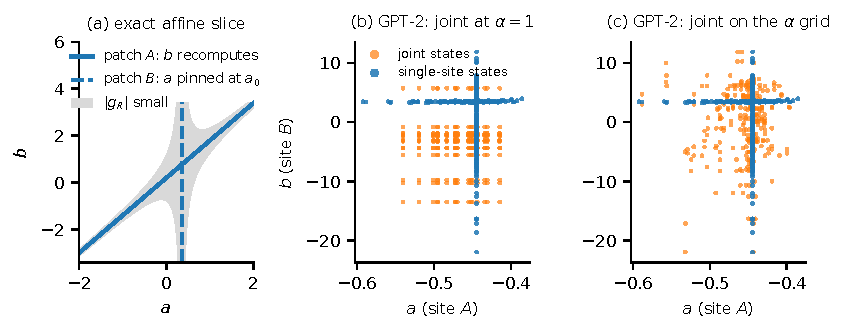
\includegraphics[width=\textwidth]{figures/fig_reachable.pdf}
\caption{Why single-site patching can leave hypothesis differences weakly constrained; $a$ and $b$ summarise the two
sites' outputs. \emph{(a)} On an exact affine slice, single-site states lie on the blue recompute and pinned arms,
where the hypothesis difference $g_R$ vanishes. The grey region, where $|g_R|$ is small, contains both arms.
\emph{(b)} One GPT-2 small IOI capture (layer pair $(5,10)$, seed $0$, unembedding chart before whitening): single-site
states (blue) form thin arms, while joint states (orange) at interpolation coefficient $\alpha=1$ spread across a region.
\emph{(c)} Matching the joint family's $\alpha$ grid to the single-site grid broadens its range in this capture. The trained-model arms illustrate
weak identification, not exact vanishing.}
\label{fig:reachable}
\end{figure}

The underlying mathematics is classical. For polynomial classes, blind spaces describe classical aliasing
\citep{pistone1996groebner}. We compare intervention families by which hypothesis differences they resolve, using the
support preorder of information matrices \citep{pukelsheim2006optimal}. Recompute versus clamp parallels total versus
controlled direct effects \citep{pearl2001direct}. Our contribution is to treat the network-produced internal states as the design points. In
classical design the analyst writes them down. Under patch-and-recompute the analyst chooses the intervention and the
\emph{network} produces the internal state, so the aliasing structure is a property of the trained model that can be
measured without observing any readout. 

Section~\ref{sec:theory} establishes what those states can separate on idealised slices.
Sections~\ref{sec:practical} to~\ref{sec:predict} study weak identification in trained models, and
Section~\ref{sec:pitfalls} examines misleading comparisons between designs. Section~\ref{sec:ioi} asks what
single-site evidence establishes about an effect at other upstream states. These questions require three distinct
kinds of evidence.

\begin{tcolorbox}[title={Three kinds of claim}]
\textbf{Exact slices} (\S\ref{sec:theory}). On the analysed two-site operator slices, in the stated polynomial
coordinates, the operator on the edge fixes the first degree with a nonzero blind difference. It is $\DstarAffine$ for
affine slices and $\DstarRMSNorm$ for the stated normalisation slices; the stated transcendental slices have no finite onset.\\[2pt]
\textbf{Trained models} (\S\S\ref{sec:practical}--\ref{sec:pitfalls}). In the tested charts and polynomial classes,
the recompute single-site and joint designs have full rank. Some directions are nevertheless much more weakly
constrained by single-site evidence than by joint evidence. This is weak identification, not exact
non-identifiability.\\[2pt]
\textbf{Transport} (\S\ref{sec:ioi}). Without a model, single-site evidence does not determine whether a component's
measured effect carries over to other states of an upstream component. Four-point interventions with the downstream output forced measure
that transport deviation directly on the tested states.
\end{tcolorbox}

We make four contributions. First, we formalise the blind space of an intervention family relative to a declared mechanism class, and separate what a single-site patch measures from the claim that this effect transports (\S\ref{sec:setup}). Second, we prove on the analysed two-site slices that the operator fixes the onset of exact blindness ($d^*=\DstarAffine$, $\DstarRMSNorm$ or $\infty$ for affine, normalisation and transcendental slices), and that for affine single-site designs at fixed $d\ge2$, the unresolved polynomial fraction grows with site count (\S\ref{sec:theory}).

Third, in a re-analysis of inspected captures, a direction named without readouts has at least $10\times$ less held-out energy under single-site than under joint patching in $\PredMTotalCount$ trained-model captures, much of it already present in the classical one-at-a-time design (\S\ref{sec:predict}); support mismatch and chart selection each invalidated one of our comparisons of intervention families (\S\ref{sec:pitfalls}). Fourth, single-site IOI evidence alone cannot determine transport. On three base prompts, the exploratory cubic predicts the contrast worse than zero; with downstream output forced, median capture RMS is small on tested grids. Replication on $\RepPrompts$ fresh prompts from $\RepTemplates$ templates met both registered smallness criteria for template medians but was floor-limited for controls, so the section stays exploratory (\S\ref{sec:ioi}). Table~\ref{tab:status} maps the claims to their status and keeps the failed and withdrawn claims visible.

\begin{table}[t]
\centering\footnotesize
\caption{Main claims and all failed or withdrawn claims, with their status; the status terms are defined in Appendix~\ref{app:limits}. \emph{Withdrawn}: retracted, either already in the submitted version (marked $^{\dagger}$) or here.}
\label{tab:status}
\begin{tabularx}{\textwidth}{@{}>{\raggedright\arraybackslash}X >{\raggedright\arraybackslash}p{0.2\textwidth} l@{}}
\toprule
claim & status & where \\
\midrule
On analysed slices, the operator on the edge fixes the onset $d^*$ ($\DstarAffine$, $\DstarRMSNorm$, $\infty$) & proved & \S\ref{sec:theory}, App.~\ref{app:proofs} \\
For affine single-site designs at fixed $d\ge2$, the unresolved fraction grows with the number of sites & proved & \S\ref{sec:theory}, App.~\ref{app:proofs} \\
\midrule
A readout-free named direction is S-weak (weakly constrained by single-site relative to joint evidence) in $\PredMTotalCount$ captures; the one-at-a-time generator meets the same threshold in $\OfatRowCount$ & empirical & \S\ref{sec:predict} \\
Support mismatch inflates reverse-escape counts ($\EdgeFrozenEscapes$ before grid matching; $\EdgeMatchedEscapes$ after); optimising a chart on the scored states creates a selection effect & empirical & \S\ref{sec:pitfalls} \\
\midrule
Single-site evidence alone does not determine the IOI transport deviation & exact & \S\ref{sec:ioi} \\
Under the cubic working model the IOI transport deviation is weakly constrained and poorly predicted & exploratory & \S\ref{sec:ioi} \\
The RMS of the executed IOI transport deviation is small on the tested grids (median over captures on three base prompts; template medians on $\RepPrompts$ fresh prompts from $\RepTemplates$ templates) & exploratory; registered smallness criteria replicated ($\RepHAbsCount$, $\RepHRelCount$ templates) & \S\ref{sec:ioi}, App.~\ref{app:replication} \\
Whether the IOI transport deviation exceeds the level of heads with no claimed role & floor-limited & \S\ref{sec:ioi}, App.~\ref{app:replication} \\
\midrule
Mutual non-domination of single-site and joint evidence; empirical mutual non-domination of recompute and clamped single-site evidence in a chart optimised on the scored states & withdrawn$^{\dagger}$ & \S\ref{sec:pitfalls}, App.~\ref{app:matched}, \ref{app:chart} \\
Specificity of single-site detection of non-additivity and its residual-bootstrap calibration; a reported number compatible with a much larger contribution; a representation no-separation claim; residual decay as a diagnostic of transcendence; auxiliary comparisons, angle stability, a Taylor check and numerical Davis--Kahan bounds & withdrawn & \S\ref{sec:ioi}, App.~\ref{app:corrections} \\
Reciprocal cross-family degradation of a frozen circuit; representation-specific weak subspaces & failed & App.~\ref{app:negatives} \\
\bottomrule
\end{tabularx}
\end{table}

% ============================================================== 2 ====
\section{What a patching experiment observes}
\label{sec:setup}

The opening example illustrates the principle: an intervention family sees a mechanism only through the states it reaches. Fix a
model and $k$ internal sites. A chart summarises the sites' outputs as a state $z\in\mathcal Z$, and a scalar readout
$y$ records behaviour (a logit difference throughout). An \emph{intervention family} $Q$ produces chart states: its
reachable set $R_Q=\{z(q):q\in Q\}$. A \emph{mechanism hypothesis} is a function $f:\mathcal Z\to\mathbb R$ that
predicts the readout. The \emph{mechanism class} $\mathcal F$ is the set of alternatives the analyst agrees to
consider. Here we take it to be a linear space of such functions.

Without a declared $\mathcal F$, ``which mechanisms are
distinguishable'' has no answer, because any finite body of evidence is consistent with infinitely many functions.
The blind space collects the hypothesis differences that vanish on every reachable state, and one family resolves at
least as much as another when its blind space is contained in the other's.

\begin{definition}[Blind space; resolving preorder]
\label{def:blind}
The evidence map $\mathrm{Res}_Q:\mathcal F\to\mathbb R^{R_Q}$, $f\mapsto f|_{R_Q}$, restricts each
hypothesis to the reachable set; its codomain is the space of real-valued functions on that set. Define
\[
  N(Q,\mathcal F)=\ker\bigl(\mathrm{Res}_Q|_{\mathcal F}\bigr),\qquad
  Q_1\succeq_{\mathcal F}Q_2 :\iff N(Q_1,\mathcal F)\subseteq N(Q_2,\mathcal F).
\]
Two hypotheses are indistinguishable under $Q$ iff their difference lies in $N(Q,\mathcal F)$. Families are
\emph{incomparable} when neither relation holds.
\end{definition}

Adding evidence can only shrink the blind space, since $N(Q_1\cup Q_2,\mathcal F)=N(Q_1,\mathcal F)\cap
N(Q_2,\mathcal F)$.

Three kinds of intervention matter here. Our interventions replace a site's complete output. For a chosen donor prompt, the coefficient $\alpha$
moves that output a fraction of the way from its clean value to its value on the donor prompt: $\alpha=0$
is clean, $\alpha=1$ is the donor, and values outside $[0,1]$ extrapolate. Under \emph{patch-and-recompute}, patching
$A$ replaces its output and lets every downstream site recompute. On an analysed two-site slice, suppose $B$'s
recomputed chart coordinate is a function $b=e(a)$ of $A$'s coordinate (the realised $A\to B$ map), and let
$a_0,b_0$ be the clean coordinates. Single-site patching then has two arms. Patching $A$ reaches $(a,e(a))$, and
patching $B$ with $A$ clean reaches $(a_0,b)$, so $R_S=\{(a,e(a))\}\cup\{(a_0,b)\}$. The graph relation is an
idealisation of the analysed slice; in trained models, Sections~\ref{sec:practical} to~\ref{sec:pitfalls} use the
recorded intervention states directly. Under \emph{clamping}, $B$ is held at its clean output while $A$ is patched.
Together with patching $B$ while $A$ stays clean, this reaches $\{(a,b_0)\}\cup\{(a_0,b)\}$. \emph{Joint} patching sets
both outputs.

Every reported effect is conditional on its prompts, sites, replacement outputs and execution semantics. We therefore
do not treat it as a context-independent contribution of a component, and \S\ref{sec:ioi} tests one such transport
claim directly.

% ============================================================== 3 ====
\section{Exact geometry on operator slices}
\label{sec:theory}

We first analyse the single-site families just defined on a two-site slice whose reachable set can be written down. Proofs are in
Appendix~\ref{app:proofs}. Here the mechanism class is the real polynomials in $(a,b)$ of total degree at most $d$,
$\mathcal F=\mathcal P_{\le d}$. The blind space is $N(Q,\mathcal P_{\le d})=I(R_Q)\cap\mathcal P_{\le d}$, where the
\emph{vanishing ideal} $I(R_Q)$ collects all polynomials that vanish on the reachable set. We write
$d^*(Q)=\min\{d:N(Q,\mathcal P_{\le d})\neq0\}$ for the \emph{onset} of exact blindness.

For the recompute single-site family on an affine edge $e(a)=ma+c$, with $b_0=ma_0+c$, every blind polynomial is a
multiple of the single \emph{generator} $g_R=(a-a_0)(b-ma-c)$, so exact blindness begins at degree $2$. The clamped
family has the degree-2 generator $g_C=(a-a_0)(b-b_0)$. Appendix~\ref{app:proofs} shows that the two designs
can have the same Hilbert profile (the number of independent constraints the evidence imposes) while missing different
hypothesis directions (Proposition~\ref{prop:incomparable}), so counts alone do not rank them. On this slice the
generators differ by $g_C-g_R=m(a-a_0)^2$.

More generally, suppose the recompute arm lies on an irreducible curve $P=0$. Single-site patching then cannot
distinguish hypotheses that differ by a multiple of $(a-a_0)P$, so exact blindness starts at degree $1+\deg P$. The
theorem states the conditions.

\begin{theorem}[Operator-slice theorem]
\label{thm:operator}
On a two-site slice, let the pinned branch be $A_0=\{(a_0,b):b\in B_0\}$ with $B_0$ infinite. Let the
recompute branch $\Gamma=\{(a,e(a))\}$ be an infinite subset of the zero set $V(P)$. Assume that $P\in\mathbb R[a,b]$ is irreducible
(not a product of two nonconstant polynomials) and not an associate (a nonzero constant multiple) of $a-a_0$. Then $I(A_0\cup\Gamma)=\bigl((a-a_0)P\bigr)$ and $d^*=1+\deg P$.
\end{theorem}

Affine edges have $\deg P=\DstarAffineDegP$, so $d^*=\DstarAffine$. For the normalisation slices
$e(a)=\beta+\omega a/\sqrt{\kappa a^2+\epsilon}$ with $\omega\neq0$, $\kappa>0$ and $\epsilon>0$, clearing the radical
gives an irreducible $P$ of degree $\DstarRMSNormDegP$, so $d^*=\DstarRMSNorm$ on these RMSNorm and LayerNorm slices:
normalisation \emph{raises} the onset. This is an exact statement about those slices, not about trained normalisation
edges in general. If no nonzero polynomial vanishes on the graph of $e$, then $I(\Gamma)=(0)$,
the blind space is zero at every finite degree, and $d^*=\infty$; a separate lemma proves this for two-key softmax
and sigmoid-gated linear-attention slices with nonzero parameters.

\begin{figure}[t]
\centering
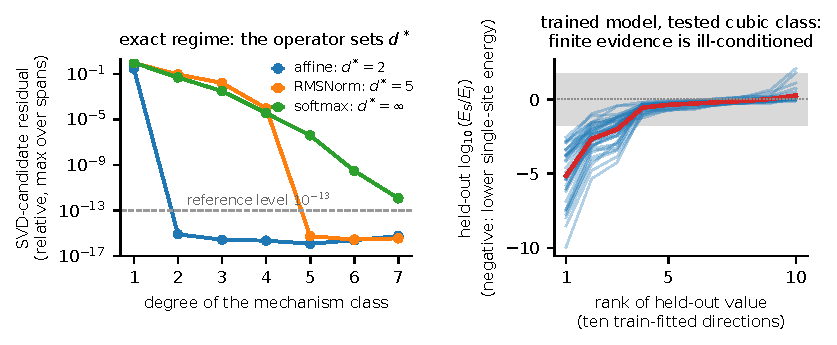
\includegraphics[width=\textwidth]{figures/fig_regimes.pdf}
\caption{Exact operator slices and a trained model. \emph{Left:} maximum relative residual of a candidate polynomial relation fitted on each operator slice (Appendix~\ref{app:limits} gives the fitting procedure). The affine and RMSNorm residuals reach numerical precision at their
proved onsets. The softmax residual decreases over the tested degrees, but numerical residuals alone cannot
distinguish exact relations from accurate approximations (Remark~\ref{rem:scope}). The dashed line is a reference
level of $10^{-13}$. \emph{Right:} GPT-2 small IOI captures, with the joint family on the same $\alpha$ grid as the single-site family
(\S\ref{sec:practical}). Both tested cubic designs are full rank, but some train-fitted directions have much lower
held-out energy under single-site than under joint interventions. The vertical axis is $\log_{10}(E_S/E_J)=-\log_{10}r$, with $r$ defined in \S\ref{sec:practical}; negative values mean lower single-site energy. Each thin line sorts one capture's held-out values in increasing order.
The thick line averages these ordered profiles. The grey band is the same-family envelope of
\S\ref{sec:practical}, shown for display.}
\label{fig:regimes}
\end{figure}

With $k$ sites patched one at a time, the reachable set is a union of $k$ curves. On arm $i$ the patched coordinate
is swept, upstream coordinates stay clean and downstream ones are recomputed from it. Assume that every coordinate on
each arm is a polynomial in that arm's swept coordinate.

\begin{proposition}[Restriction-rank bound for polynomial single-site arms]
\label{prop:ksite}
Let the coordinates on arm $i$ be polynomials $z_{ij}(t)$ of the swept coordinate $t$, with $z_{ii}(t)=t$, and let
all arms pass through the clean configuration. Set $\eta_i=\max\bigl(\{1\}\cup\{\deg z_{ij}:z_{ij}\text{
nonconstant}\}\bigr)$. Then $\operatorname{rank}(\mathrm{Res}_Q|_{\mathcal P_{\le d}})\le1+d\sum_i\eta_i$, so
$\dim N(Q,\mathcal P_{\le d})\ge\binom{d+k}{k}-\bigl(1+d\sum_i\eta_i\bigr)$.
\end{proposition}

The degrees must include all downstream recomputation (Appendix~\ref{app:proofs}). For affine edges $\eta_i=1$ and the
bound $1+kd$ is attained, while the polynomial class grows much faster with the number of sites. At degree $3$, the
unresolved fraction rises from $\KBlindTwo\%$ at two sites to $\KBlindFive\%$ at five. A joint Cartesian product with
at least four distinct values on each axis resolves all of it.

\begin{remark}[Continuum, not grid; slice, not network]
\label{rem:scope}
Exact $d^*$ statements concern the operator's continuum of reachable states: every finite grid admits vanishing
high-degree polynomials, so numerical checks corroborate but never establish these algebraic claims.
The statements concern analysed two-site slices in the chosen polynomial coordinates, \emph{not} whether a full
transformer has or lacks exact blind mechanisms.
\end{remark}

In the trained-model charts and polynomial classes we evaluate, the recompute single-site and joint designs have no
exact blind direction. The next section therefore asks how weakly they constrain different directions.

% ============================================================== 4 ====
\section{From exact blindness to weak identification}
\label{sec:practical}

The exact results above concern operator slices; Sections~\ref{sec:practical} to~\ref{sec:pitfalls} turn to trained models. For the recompute single-site and joint
designs, in every capture, chart and class we evaluate, the exact blind space is trivial: both designs have full
rank. The question is therefore graded: how much less does a hypothesis difference vary under one family than under
another? These are statements about weak identification in the evaluated charts and classes, not about exact
non-identifiability. The clamped comparison family of \S\ref{sec:pitfalls} is the one exception, because its pinned
coordinate arms give it an exact polynomial kernel by construction (Appendix~\ref{app:protocol}).

We measure how visible a hypothesis difference is by its mean square on the states a family reaches. Let $\mu_Q$ be
the measure that weights the states of $Q$, let $\varphi$ be a feature map spanning $\mathcal F$, and let
$G_Q=\mathbb E_{\mu_Q}[\varphi(z)\varphi(z)^\top]$ be the intervention Gram operator. A hypothesis difference
$h=\theta^\top\varphi$ then has \emph{energy} $E_Q(h)=\theta^\top G_Q\theta=\mathbb E_{\mu_Q}[h^2]$. Small energy
means that the hypotheses differ little on those states. Under the regularity conditions that hold for the polynomial classes used here (continuous features, finite second
moments, and $R_Q=\operatorname{supp}\mu_Q$), the kernel of $G_Q$ is exactly the blind space. Energy therefore gives a
graded analogue of exact blindness.

For a fixed hypothesis difference, or direction, $h$ we report the \emph{held-out $J/S$ energy ratio}
$r(h)=E_J^{\mathrm{te}}(h)/E_S^{\mathrm{te}}(h)$, where $S$ and $J$ are the single-site and joint families. A large
ratio means that single-site evidence constrains $h$ much less than joint evidence does, and we call such a direction
\emph{S-weak}. ``Held-out'' means that the direction is fitted or named on training rows and scored on the
complementary rows: the rows of each design are split in half, and directions are frozen before scoring. For the named
direction of \S\ref{sec:predict}, the edge fit, whitening and feature scaling use training rows only. The archived
optimised profiles instead used all analysed rows for whitening and scaling. For the fixed polynomial basis and
covariant eigensolve, Appendix~\ref{app:protocol} shows that this is only a change of feature basis in exact
arithmetic and leaves the held-out profiles unchanged. To find directions with contrasting energies, we form the Gram operators on training rows and solve the regularised generalised
eigenproblem
\[
  \bigl(G_S+\lambda G_{\mathrm{ref}}\bigr)w=\nu\,\bigl(G_J+\lambda G_{\mathrm{ref}}\bigr)w,\qquad
  G_{\mathrm{ref}}=\tfrac12(G_S+G_J),\quad\lambda=10^{-6},
\]
which regularises both sides by the same covariant reference operator, so that a change of feature basis leaves the
spectrum invariant (Appendices~\ref{app:protocol} and~\ref{app:noninvariant}). The held-out profile orders the log
single-site-to-joint energy ratios of all frozen training eigen-directions on test rows. Its low end is S-weak;
its reverse end is joint-weak.

We analyse $\MatchedN$ float32 captures across $\PredCells$ model--task cells; a capture is one run for a pair of
sites and a seed. Captures share prompts and tasks, so counts are consistency checks and we make no population claim.
The degree-3 polynomial class, the intervention grids and the chart are described in Appendix~\ref{app:protocol}. A
readout screen excludes captures with $\mathrm{sd}(Y_{\mathrm{joint}})<0.15$; it is the only use of readouts in
Sections~\ref{sec:practical} to~\ref{sec:pitfalls}, and it makes the analysed sample readout-conditioned.

Optimising a direction can produce extreme ratios even within one family, so we rerun the train--freeze--score procedure on two splits of the single-site family and use their held-out profiles as a \emph{same-family envelope}. Escape counts are descriptive and any $p$-values are nominal (Appendix~\ref{app:protocol}, which gives the exact construction).

% ============================================================== 5 ====
\section{A weak direction predicted from intervention geometry}
\label{sec:predict}

Is single-site weakness only an artefact of searching for a weak direction? To find out, we score the one direction
the theory names without any search. On an affine slice the single-site blind space is generated by
$g_R=(a-a_0)(b-ma-c)$. We estimate it from intervention states alone: from the training rows, $a_0$ comes from
the downstream-patching arm and $(m,c)$ from a least-squares fit of $b$ on $a$ along the upstream arm. No readout
enters, and the direction is not chosen to separate the families. This is a re-analysis of captures we had inspected
earlier with an optimised procedure; we ran no fresh validation of the named direction.

The held-out $J/S$ energy ratio of this direction exceeds $10\times$ in
$\PredMTotalCount$ captures across $\PredCells$ cells. Appendix~\ref{app:units} gives the per-cell medians
(Table~\ref{tab:predict}) and three further checks (donor indices held out, summaries by prompt group, random directions),
which give the same qualitative picture. A classical one-at-a-time baseline explains much of this. The clamped generator
$g_C=(a-a_0)(b-b_0)$ is the blind generator of the one-at-a-time design, and it vanishes on both of that design's
arms. On an exact affine slice it equals $m(a-a_0)^2$ on the recompute arm. It is small when the edge is flat and the
scatter low, and most edges in this chart are flat (Appendix~\ref{app:matched} gives the finite-capture expression).
Scored on the same recompute single-site and joint states, $g_C$ also clears $10\times$ in $\OfatRowCount$ captures.
The recompute generator exceeds this baseline count by a net $\OfatNetDifference$ captures.

Relative to the one-at-a-time baseline, the recompute generator becomes more distinctive as the fitted edge gets
steeper: $r(g_R)/r(g_C)$ increases with the absolute whitened edge slope (Spearman $\OfatSpearman$). Its absolute
ratio $r(g_R)$ nevertheless falls as the edge strengthens (Spearman $\EdgeBlindRho$ over $\EdgeN$ captures), where
edge strength $s$ is $\mathrm{sd}(b\mid\text{arm }A)/\mathrm{sd}(b\mid\text{arm }B)$ on training single-site rows.
The largest ratios therefore come from captures where $A$ barely drives $B$. Our attempt to remove this dependence by
choosing the chart failed (\S\ref{sec:pitfalls}); Appendix~\ref{app:matched} gives the remaining edge diagnostics.

On an analysed algebraic slice the candidate can be named by construction; whether it is weak in a finite trained-model sample, and by how much, is an empirical question (Appendices~\ref{app:robust} and~\ref{app:three}). The normalisation onset $\DstarRMSNorm$ applies only to the analysed normalisation slice, not to a trained edge.

In these captures, single-site evidence has a weakly constrained direction that geometry can name from one sweep of
intervention states. That does not show that the single-site family is worse than every other family, and such
comparisons are easy to get wrong, as the next section shows.

% ============================================================== 6 ====
\section{Two traps when comparing intervention families}
\label{sec:pitfalls}

The comparison above raises a further question: could intervention families look differently informative for reasons
unrelated to the mechanism of interest? We encountered two such artefacts in our own comparisons. The corrected analyses follow, and the claims they overturned are
withdrawn (Table~\ref{tab:status}).

\paragraph{Unmatched supports.} Our single-site family sweeps $\alpha\in[-0.5,1.5]$, extending half the clean-to-donor
distance beyond each endpoint, while the joint family used raw donors ($\alpha=1$). A polynomial that is large only in
the extrapolated region then looks ``visible to $S$, weak under $J$'' for reasons unrelated to any mechanism. The
same-family null cannot detect this, because both halves of $S$ share the same support. This mismatch underlay our withdrawn claim that single-site and joint evidence are \emph{mutually non-dominating},
that is, that a reverse direction also exists, weakly constrained by joint evidence and well constrained by
single-site evidence. We therefore recollected the joint family
on the same $\alpha$ grid, with the same prompts, donors and weights. Reverse escapes above the same-family envelope
fell from $\EdgeFrozenEscapes$ captures to $\EdgeMatchedEscapes$, and restricting both families to $\alpha\in[0,1]$
leaves $\EdgeSymmetricEscapes$. The few remaining reverse escapes are descriptively associated with stronger edges
(Appendix~\ref{app:matched}). The matched joint family is a sparse design on the same grid, not a product grid, so
exact support matching is not established; the comparison uses paired float32 captures. The lesson: before comparing
two intervention families, check that their reachable sets span the same region. 

\paragraph{Selecting a chart on the evaluation states.} To make the recompute and clamped single-site designs differ,
the edge must be non-flat, and in the unembedding chart it is nearly flat (median absolute whitened slope
$\RCUchartChartM$). We therefore selected the downstream coordinate by maximising a readout-free, regularised variance ratio between the
two arms, and compared recompute with clamped single-site evidence in that chart. The recompute-weak end of the optimised profile then escaped the same-family envelope in
$\RCPooledR$ captures. With a chart fitted on a different seed of the same layer pair it escaped in
$\RCXseedPooledR$. The two analyses cover different cohorts (Appendix~\ref{app:chart}), so this is not a paired
effect estimate. The selection rule helps explain the failure. For GPT-2 its denominator was estimated from at most
$16$ donor directions in a $768$-dimensional activation space. In the GPT-2 captures for which this was logged, the
selected direction had numerically negligible projection onto the span of those donor directions.  We withdraw the claim of non-domination in a chart optimised on the scored states. The
lesson: optimising a chart on the states where it is scored is a selection effect, even when no readout is consulted.
Fit the chart on different prompts and donors from those on which it is scored.

These traps show why an intervention comparison must specify the states it reaches. The next section asks what those
states can establish about a single measured effect, the kind a circuit analysis reports.

% ============================================================== 7 ====
\section{Does a measured effect carry over? A published IOI edge}
\label{sec:ioi}

Does a Name Mover head's measured single-site effect carry over to other states of an upstream S-Inhibition head? We
ask this on the S-Inhibition $\to$ Name Mover edge of the IOI circuit of \citet{wang2022ioi} in GPT-2 small.
Interpreting a single-site effect as a contribution that persists across upstream states assumes that it does. This is
the practical form of the blind-space question, because a single-site run never visits the states where the effect would
have to hold. Because our test forces the Name Mover's output, it asks only how the readout combines the two heads' outputs on the
executed states. It does not test the query-mediated pathway by which S-Inhibition changes what the Name Mover
writes, and it does not contradict the mechanism \citet{wang2022ioi} identified by path patching.

\begin{tcolorbox}[title={The transport contrast}]
The question is simple: does $B$ have the same measured effect after $A$ changes? Write $u$ and $v$ for replacement
outputs of $A$ and $B$, and $0$ for each site's clean output (so $u=0$ corresponds to $a=a_0$). $Y(u,v)$ is the
readout with $A$'s output set to $u$ and $B$'s output forced to $v$; $Y(u,0)$ keeps $B$ at its clean output. Patching
$B$ alone measures its effect \emph{in the context} where $A$ is clean,
\[
  \Delta_B(v)=Y(0,v)-Y(0,0).
\]
If this effect transports to the upstream state $u$, the same $\Delta_B(v)$ should apply once $A$ is changed to $u$.
Exactly, and without any model,
\[
  Y(u,v)-Y(u,0)=\Delta_B(v)+T_C(u,v),\qquad T_C(u,v)=Y(u,v)-Y(u,0)-Y(0,v)+Y(0,0).
\]
The four-point (difference-in-differences) \emph{transport contrast} $T_C$ uses the clamped corner $Y(u,0)$, and it
vanishes at every tested $(u,v)$ exactly when $B$'s measured effect carries over to every tested state of $A$.
Patching $A$ alone observes $Y(u,v_{\mathrm{rec}}(u))$, where $v_{\mathrm{rec}}(u)$ is the output $B$ recomputes to; it
generally observes neither the joint corner $Y(u,v)$ nor the clamped corner $Y(u,0)$. Single-site evidence therefore
does not determine $T_C$ without additional assumptions. Executing the two missing corners measures it directly and
needs no chart.
\end{tcolorbox}

\paragraph{Design.} We pair four S-Inhibition heads with three Name Movers (twelve published head pairs). Controls
pair four early heads that have no claimed IOI role with the same Name Movers. A \emph{head pair} with a prompt is a
capture; on three base prompts, $\QCN$ of the $36$ published captures and $\QCCtrlN$ of the $36$ control captures
pass the screen. Each capture executes the single-site arms, the clamped arm and $256$ joint states;
Appendix~\ref{app:ioi} lists the head identities.

\paragraph{The executed contrast is small on the tested grids.} This analysis was chosen after seeing the data, so we
call it exploratory. For each capture on the three base prompts we compute the root mean square (RMS) of $T_C$ over
the tested joint states. The median RMS over captures is $\AdqRmsT$ logits. Dividing each capture's RMS by its
\emph{B-arm swing} gives a median percentage of $\AdqRmsTPct\%$. The swing is the readout range over the single-site $B$ arm ($32$ donors $\times$ $\NAlpha$
coefficients; median $\MfSwingMed$ logits, never below $\MfSwingMin$). The largest single $|T_C|$ in a capture is $\MfMaxAbsMax$
logits at most, so smallness describes the RMS over states, not every state. These captures do not measure the
numerical floor; Appendix~\ref{app:ioi} gives the spread and a second normalisation.

\paragraph{A preregistered replication meets both registered smallness criteria.} Before collecting fresh data, we
preregistered a replication (Appendix~\ref{app:replication}). It used $\RepPrompts$ new prompts, three from each of $\RepTemplates$ IOI
templates of \citet{wang2022ioi} that our earlier captures had not used, with the same head pairs, controls, design
and analysis. For each prompt we take the median RMS of $T_C$ over its screened published captures. For each template
we then take the median of its three prompt medians ($V_t$), and likewise for the percentage of the swing
($V_t^{\mathrm{rel}}$). $V_t$ was below $\MfMargin$ logits in $\RepHAbsCount$ templates and $V_t^{\mathrm{rel}}$ below
$1\%$ in $\RepHRelCount$, so both registered smallness criteria passed. Both margins were set after the exploratory
analysis, and the relative one is the informative criterion. Registered smallness concerns template medians, not
every capture; individual captures can be larger (Appendix~\ref{app:replication}).

\paragraph{The control comparison is unresolved.} The replication also measured the float32 floor by re-executing every
corner family in a different batch composition. Published contrasts exceeded ten times their floor in
$\RepPubResolved$ captures, whereas control contrasts did so in only $\RepCtlResolved$. The registered comparison of
published and control contrasts (H2) was therefore floor-limited under the registered rule. We report no
published/control ratio and make no above-control claim, and under the registered decision rule this section remains
exploratory, with its smallness replicated as registered.

\paragraph{What single-site evidence leaves unmeasured.} Single-site interventions do not execute all the corners that define $T_C$, so without a model they cannot determine it. What can a model recover? The exploratory working model is the cubic class in a fixed, weight-derived chart motivated by the published claim that S-Inhibition heads act on the Name Movers' \emph{query} (Appendix~\ref{app:limits} defines the chart), with additive terms in $a$ or $b$ alone and cross coefficients $\gamma$ on $ab$, $a^2b$ and $ab^2$. Under it $T_C(u,v)=D(u,v)^\top\gamma$, where $D$ is the four-point contrast of the cross monomials, and the additive terms cancel. On the recompute arm of an affine edge the cross terms reduce to functions of $a$ alone, which the additive terms absorb, so single-site data inform $\gamma$ only through the scatter of $b$ about the fitted edge. The \emph{design gap} is the joint/single-site ratio of smallest eigenvalues of per-observation Grams of cross terms residualised against additive terms in this chart (Appendix~\ref{app:ioi}). This measures design geometry, not Fisher information about the network.

\paragraph{On the exploratory captures, the working model does not predict the executed contrast.} Fitted on
single-site states, the cubic predicts held-out joint readouts far worse than a constant (median $R^2$ $\RespSJR$),
while an additive-only refit transfers (median $R^2$ $\RespAddThreeSJ$). Its median held-out RMS error in predicting
$T_C$ is $\MfSThree$ logits, against $\MfZero$ for predicting zero. The bootstrap interval for the excess over
predicting zero lies wholly above zero in $\MfSWorse$ single-site and $\MfJWorse$ joint fits. The model is misspecified
on both supports; only the executed contrast is model-free. Table~\ref{tab:scales} in Appendix~\ref{app:ioi} gives the
fit statistics.

For each joint state we also compute the largest $|T_C|$ inside the fit's nominal $95\%$ Wald region for $\gamma$ under
the working model, and summarise these by their median within each capture. We call this a working-model
identification width. Because the cubic is misspecified, it is neither an observed error nor a calibrated bound: the
pointwise envelopes contain the executed $|T_C|$ at every joint state in only $\AdqCoverUpperS$ (single-site) and
$\AdqCoverUpperJ$ (joint) captures. Against the B-arm swing, the median single-site working-model identification
width is $\MisS\%$ and the joint one $\MisJ\%$.

\paragraph{Single-site rejections did not detect the executed deviation.} The submitted version read the rejections of
$\gamma=0$ by single-site evidence as detection that separates published from control heads. That specificity depends
on the covariance estimator, and we withdraw it; Appendix~\ref{app:ioi} gives the counts under alternative
covariances. More fundamentally, because the cubic is misspecified on both supports, rejecting its additive
restriction is not a measurement of the executed transport contrast. Figure~\ref{fig:scales} makes the mismatch
visible: the single-site working-model width is far larger than the executed RMS deviation, while the joint width is
closer in scale but poorly calibrated. Neither can be read as a resolved measurement of $T_C$.

\begin{figure}[t]
\centering
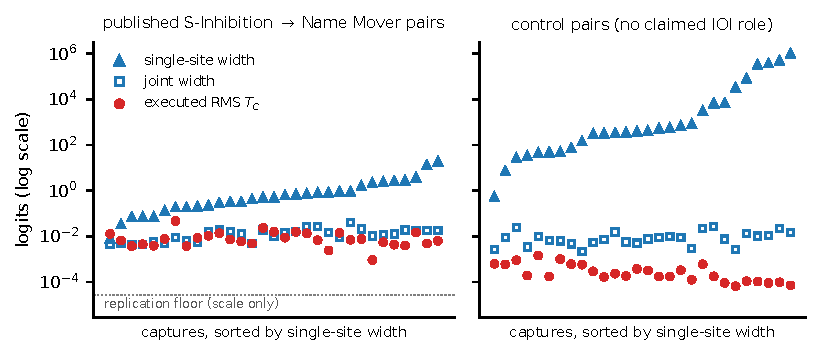
\includegraphics[width=\textwidth]{figures/fig_scales.pdf}
\caption{Working-model identification widths and executed transport contrasts, per capture (exploratory; three base
prompts). Left: published S-Inhibition $\to$ Name Mover captures; right: control captures. Captures are sorted within each panel. Triangles and open squares show the single-site and joint working-model identification widths, each a median over joint states; circles show the RMS of the executed $T_C$ over those states (log scale, logits). For the published heads, the median single-site width divided by the median executed RMS is
$\AdqEnvSOverRmsT$: the executed RMS is much smaller than the single-site width. The widths are properties of the misspecified working model, neither observed errors nor
calibrated bounds. The exploratory control captures did not measure their numerical floor. The dotted line is only a
scale reference, the median floor measured in the replication for its published captures. The plot supports no
above-control conclusion.}
\label{fig:scales}
\end{figure}

\paragraph{Scope.} Everything here concerns GPT-2 small, the published S-Inhibition $\to$ Name Mover head pairs, output-replacement interventions and the tested grid of states. Without executing the corners one cannot know whether a transport deviation is small or large; measuring it requires the clamped and joint corner families in addition to the single-site arms. Appendix~\ref{app:ioi} also reports a second head group (previous-token and induction heads), which is not a second query-mediated circuit.

% ============================================================== 8 ====
\section{What an audit should record}
\label{sec:limitations}

The geometry and IOI analyses give a checklist for auditing new patching evidence. Its limits: the exact theorems cover only the analysed operator slices, and the trained-model results concern weak identification in the evaluated charts and classes, not exact non-identifiability; the $\MatchedN$ captures share prompts and tasks, so we make no population claim. In the preregistered IOI replication on $\RepPrompts$ fresh prompts from $\RepTemplates$ templates, H1 (absolute) and H1 (relative) passed in $\RepHAbsCount$ and $\RepHRelCount$ templates, whereas H2, the published/control comparison, was floor-limited, so we report no published/control ratio or above-control claim. The section remains exploratory, and the cubic working model's identification widths are uncalibrated. Appendix~\ref{app:limits} lists the limitations in full.

\begin{tcolorbox}[title={An audit checklist for patching evidence}]
\begin{enumerate}[leftmargin=1.4em,itemsep=1pt,topsep=1pt,parsep=0pt]
\item Declare the mechanism class and the chart before using readouts to tune either.
\item Record the intervention \emph{states}, not only the readouts, and inspect each family's low-energy directions (Appendix~\ref{app:protocol}).
\item Match the regions that families reach; fit any data-derived chart on prompts and donors distinct from those used for scoring.
\item Test a working model on held-out executed contrasts and check its calibration before reading its intervals; keep rejections separate from effect estimates.
\item For a transport claim, declare the tested states, aggregation unit and margins, execute the four-point contrast, and measure its numerical floor by re-execution under a different batch composition.
\item Record when the class, chart, direction and decision criteria were fixed relative to data inspection, and separate exploratory re-analysis from preregistered evaluation.
\item Account for unequal arm variances and donor dependence; use inference units suited to the design and state the dependence that remains.
\end{enumerate}
\end{tcolorbox}

An activation-patching experiment supports a mechanistic claim only relative to the alternatives its reachable states can separate. Within a declared mechanism class, those states fix which alternatives are exactly unresolved and reveal directions that are only weakly constrained, with no readout needed. Whether a per-component effect transports is a separate question: execute the missing corners, because better single-site statistics cannot determine it without a model.

\clearpage
\bibliographystyle{plainnat}
\bibliography{refs}

\appendix
% GENERATED by make_appendix_a.py from corrections_ledger.json -- do not edit by hand.
\section{Correction log}
\label{app:corrections}

The version submitted for review contained errors that we found after acceptance. Each
row below is one entry of a correction ledger (57 entries). For each entry the ledger records an independent
verification check appropriate to the correction (recomputation, mathematical checking or inspection) and, where
applicable, the source artifacts, scripts and cited files by hash and the command or inspection behind the
correction; associated review files record the adversarial verdicts. This table is generated from that ledger. The last column states
whether a scientific conclusion changed. All other numbers in this paper are the corrected ones.

{\scriptsize
\setlength{\tabcolsep}{3pt}
\renewcommand{\arraystretch}{1.15}
\begin{longtable}{@{}>{\raggedright\arraybackslash}p{0.035\textwidth}>{\raggedright\arraybackslash}p{0.13\textwidth}>{\raggedright\arraybackslash}p{0.2\textwidth}>{\raggedright\arraybackslash}p{0.25\textwidth}>{\raggedright\arraybackslash}p{0.2\textwidth}>{\raggedright\arraybackslash}p{0.13\textwidth}@{}}
\toprule
id & item & accepted version & this version & cause & conclusion changed? \\
\midrule
\endfirsthead
\toprule
id & item & accepted version & this version & cause & conclusion changed? \\
\midrule
\endhead
C01 & Named-direction count and cell medians (Table~\ref{tab:predict}) & $172/185$ captures above $10\times$; Qwen3-8B medians $86.6$ (IOI) and $91.4$ (induction) & $171/185$; $60.0$ and $66.4$; every cell median recomputed with the edge fitted on training rows & the edge (a0, m, c) was fitted on rows that included the held-out half (the whitening leak cancels from this ratio) & No (procedure corrected) \\
C02 & Random-direction null (Table~\ref{tab:predict}) & 95th percentiles $3.99$--$14.0$ & cell medians of capture-specific 95th percentiles $7.02$--$11.4$ on the same captures and split; the named direction beats its own capture's null in $180/185$ & null range taken from different (unmatched, raw-donor) captures and an all-rows fit & Magnitude only \\
C03 & Donor-level robustness & $168/185$ captures under a ``stricter whole-donor split'' & that test scored the optimised direction and counted escapes of the same-family envelope; with both donor indices held out, the named direction's held-out $J/S$ energy ratio is above $10\times$ in $173/185$ captures; donor content is not held out (identical patch-$A$ trajectories cross the partition in $72/185$ captures) & a different direction, partition, null and criterion were reported as the named direction's donor test & No (procedure corrected) \\
C04 & Prompt-level robustness & $25/38$ prompt groups; bootstrap lower bound $0.856$ & row-split named direction: every capture above $10\times$ in $28/38$ (cell, prompt) groups; a bootstrap over groups gives $87.4$\% as the lower end of a 95\% percentile interval for the pooled fraction of captures above $10\times$ & prompt-level analysis scored the optimised eigenvector, not the named generator & No (procedure corrected) \\
C05 & IOI envelope: the four-point contrast & single-site $42.9$\% vs joint $0.779$\% (ratio $55.1$) ``of the reported number''; exceeds the whole number in $11/31$; synthetic self-test coverage $97.7$\% & working-model Wald envelopes of $31.1$\% vs $0.764$\% of the B-arm swing ($40.6$); the single-site envelope exceeds the whole swing in $9/31$; envelopes contain the executed $T_C$ at all states in $12/31$ and $1/31$ captures; synthetic self-test coverage $97.3$\% & the code evaluated two of the four terms of the stated contrast & Yes: interpretation \\
C06 & Denominator of the IOI percentage & ``of the reported number'', read as $Y(a_0,b)-Y(a_0,b_0)$ & the B-arm swing (median $1.65$, minimum $0.67$ logits) & the prose named a different denominator from the one the code used & Yes: interpretation \\
C07 & Size of the contribution a reported number is compatible with & a per-component number on these heads is compatible with a substantially larger contribution & withdrawn; post-review exploratory analysis on three base prompts: the executed $T_C$ is small on the tested grid (median RMS $0.00709$ logits, $0.427$\% of the B-arm swing), and the single-site fit predicts it worse than zero in $31/31$; the preregistered replication on $24$ fresh prompts from $8$ templates met the absolute and relative smallness criteria for template medians of prompt medians over screened published captures on its tested grids ($8/8$ and $8/8$ templates, respectively); the control family was floor-limited ($111/268$ control captures resolved, failing the registered resolution gate), so no above-control comparison is made & an upper envelope under a working model that does not transfer was read as a plausible contribution & Yes: claim withdrawn \\
C08 & Specificity of single-site detection & published $26/31$ vs controls $0/28$ reject; ``not calibration failure'' & under alternative covariances published $26$--$29$, controls $8$--$16$, induction group $7$--$10$; covariance-sensitivity calculations for a misspecified model, not a validated calibration & one pooled homoskedastic residual variance across arms with very different variances & Yes: claim withdrawn \\
C09 & Residual-bootstrap calibration argument & null size $6.42$\% (single-site), $5.9$\% (joint) & residuals pooled across arms whose variance ratio is $0.522$ (published) and $0.00231$ (controls); argument withdrawn & the null resampled residuals across heteroskedastic arms & Yes: claim withdrawn \\
C10 & Joint coefficient ``consistent with zero'' & $|c|/\mathrm{se}$ of $1.08$ (IOI), $0.91$ (induction), $0.979$ (controls) & a ratio of norms, not a test; with the marginal-sum donor covariance $V_{\mathrm{up}}+V_{\mathrm{down}}$ (no intersection term or cross-role dependence; calibration unknown) the joint Wald test rejects in $1/31$ published and $1/28$ control configurations & a norm ratio was read as a t-statistic & Yes: interpretation \\
C11 & Pseudo-replicated $p$-values & edge contrast $p=2.35\times10^{-11}$; head-group Spearman $p=9.57\times10^{-51}$ & heads as units, as descriptive conditional permutation summaries (heads share target heads, prompts and the model): exact $p=0.0143$; $\rho=-1$, $p=2.76\times10^{-7}$ one-sided, $5.51\times10^{-7}$ two-sided & configurations sharing source heads, Name Movers and prompts treated as independent & No (inferential unit and test changed) \\
C12 & Operator-slice theorem hypothesis & $C$ Zariski-dense in an irreducible $V(P)$ & $P$ irreducible and not an associate of $a-a_0$, the recompute branch an infinite subset of $V(P)$; counterexample $P=(b-ma-c)^2$ & irreducibility of the zero set was assumed where irreducibility of P is needed & Yes: theorem scope (the stated affine, normalization and transcendental instances are unchanged) \\
C13 & Equal-Hilbert-profile proposition & condition $(m,c)\neq(0,b_0)$; statements for every $d$ & condition equivalent to $m\neq0$; incomparability needs $d\ge2$; intersection dimension $0$ for $d<3$ & missing degree restrictions & No (range repair) \\
C14 & $k$-site chain counterexample & bound $44$ vs rank $50$ & per-edge bound $41$ vs exact rank $59$ ($61$ with per-arm edges) & naive sum reported as the bound; floating-point rank & No \\
C15 & Concentration constant; eigengap sentence & intrinsic-dimension Bernstein with $L=\log(2d_{\mathrm{int}}/\delta)$; ``ill-conditioned means the relative eigengap is small'' & the two-sided bound needs a factor $8\,\mathrm{intdim}$ and holds above a threshold; ill-conditioning does not imply a small eigengap & wrong constant; a false equivalence & No \\
C16 & Appendix edge statistics & $82$ captures; Spearman $-0.936$; strong-edge median $130$ & $185$ captures; $-0.869$; $38.7$; every edge statistic recomputed & legacy pipeline (unmatched captures, all-row fits) and a changed clamped-baseline definition & Procedure and baseline corrected; qualitative association retained \\
C17 & Unmatched-table medians (Table~\ref{tab:predict-unmatched}) & for example GPT-2 IOI $7115$ & $6489$; every median recomputed with training-only fits & same held-out leak as C01 & No (procedure corrected) \\
C18 & Figure labels; the ratio in Figure~\ref{fig:reachable}(b) & plotted low end labelled ``theory-named''; the text quoted a median range ratio for the plotted capture & plots show held-out order statistics of optimised directions; the panel ratio $1.64$ is one capture, the capture median $1.86$ & plotted quantity and aggregation misdescribed (round-1 replacement label was itself wrong) & Yes: labels and supported direction corrected (descriptive plots retained) \\
C19 & Support-matching caption & only the symmetric protocol retains a significant reverse direction & the interior protocol also does (GPT-2 induction $q=7.68\times10^{-50}$; Qwen3.5 induction $q=5.15\times10^{-7}$); $q$-values nominal & caption contradicted its own table & No \\
C20 & Preregistration status & four pre-registered hypotheses failed & four planned hypotheses did not survive (two failed their criteria, two were withdrawn); dated records exist for two & preregistration status not verifiable from the version history & No \\
C21 & Readout screen & no readout values used; screened trials reported rather than dropped & the analysed sample is readout-conditioned by the screen; the IOI collector did not record dropped configurations & readout-conditioned sample selection; rejected configurations not recorded & Yes: interpretation (sample selection disclosed) \\
C22 & Induction head group & query-mediated in the same sense as IOI & reads through keys (K-composition), which a final-position query chart does not test; relabelled & mechanism mislabelled & Yes: interpretation \\
C23 & Mediator-interaction appendix & normalised interaction $3.38\times10^{-4}$--$0.0366$ over $9$ configurations & no generating script; removed & unreproducible from released code & Yes: claim withdrawn \\
C24 & Summary-block provenance & information ratio $2.68\times10^{4}$ and se ratio $72.3$ from a block written by unshipped code & the same values ($2.68\times10^{4}$, $72.3$) regenerated from rows by released code & summary block written by unshipped code & No \\
C25 & One-at-a-time baseline & no systematic baseline in the prediction table; the appendix reported $g_C$ only among strong-edge captures & $g_C$ above $10\times$ in $144/185$; both $143/185$, only $g_R$ $28/185$, only $g_C$ $1/185$, neither $13/185$; both generators scored on the same recompute single-site and joint states & missing systematic baseline & Addition \\
C26 & Scope and model names & ``three models and five behaviours''; ``Qwen3.5'' & ten model $\times$ task cells; GPT-2 small, Qwen3.5-9B-Base, Qwen3-8B & scope statement compressed; model names abbreviated & No (clarification) \\
C27 & ``Predicted prospectively'' & a prospective prediction & named from training states without readouts; a re-analysis of inspected captures & temporal claim not supported by the record & Yes: interpretation \\
C28 & Bibliography & Lin and Liu at ICML; Makelov et al.\ with three authors; unstated versions & arXiv preprint; the conference version with four authors; versions stated & one wrong venue, one author list from a different version, two version choices & No \\
C29 & ``The misattribution is the blind generator'' & $c(a-a_0)(b-b_0)$ is the blind generator of the framework & that is $g_C$, equal to $g_R$ only modulo additive terms; the link goes through the transport identity & two generators conflated & Yes: interpretation \\
C30 & Path-patching appendix & a path-patching family summary & no generating script; removed & unreproducible from released code & Yes: claim withdrawn \\
C31 & ``Fisher information'' & partial Fisher information ratio $2.68\times10^{4}$ & a residualised design-Gram ratio: $2.68\times10^{4}$ (median), $2.42\times10^{4}$ (ratio of medians); a plug-in homoskedastic Fisher ratio of $1.49\times10^{4}$ uses residual variances that are not a validated noise model & a design Gram was called Fisher information & Yes: information interpretation (a fixed-chart geometric gap remains) \\
C32 & Same-family null $p$-values & binomial $p$ against the nominal escape rate calibrates the procedure & the null runs at a different sample size and captures share prompts; $p$-values nominal & null built at a different sample size; independence assumed & Yes: interpretation (p-values nominal) \\
C33 & bfloat16 captures & affects the readout only & recorded states also carry bfloat16 rounding (GPT-2 IOI and Qwen3.5 unmatched captures) & model dtype propagates into the recorded states & No (description corrected) \\
C34 & Coefficient-space angles & direction agreement $0.814$$^\circ$ and $1.87$$^\circ$ & parameterisation-dependent; removed & parameterisation-dependent quantity used against the paper's own rule & Yes: claim withdrawn (auxiliary) \\
C35 & Matched joint family & a product grid & a sparse design on the same $\alpha$ grid & design described by its idealisation & Yes: interpretation and scope (same alpha grid and descriptive counts retained; exact support matching not established) \\
C36 & Cross-seed chart control & ``a different prompt and a disjoint donor set'' ($103/170$ to $26/120$) & the same prompt in $10/120$ captures; donors drawn with replacement from a shared pool, so content disjointness is not established & a seed change was described as disjoint content & Yes: interpretation (control scope) \\
C37 & Gram kernel and blind space & $\ker G_Q=N(Q,\mathcal F)$ when $R_Q=\operatorname{supp}\mu_Q$ & equality holds if the features are continuous with finite second moments (a sufficient condition); in general the Gram kernel is the almost-everywhere blind space & a regularity assumption was left implicit & No (assumption stated) \\
C38 & Davis--Kahan eigengap & relative eigengap $0.127$ and $0.0813$ at the low-energy boundary; bounds $39.9$ and $46.6$ & those gaps were taken at the top of the spectrum; at the bottom-3 boundary the joint-family gaps are $0.00295$ and $0.00317$; the bounds are vacuous a fortiori and their numbers withdrawn & eigengap indexed at the top of an ascending spectrum while the bottom eigenspace was compared & No (the bounds were already reported as vacuous; the numbers are withdrawn) \\
C39 & Legacy robustness checks & ``the frozen procedure under four charts''; a Taylor row that reproduces the polynomial row ``as the proposition requires'' & Euclidean ridge with all-row whitening, so not held-out validation; the difference chart is the pooled intervention mean minus clean; the Taylor row duplicates the polynomial design (zero centre) and is removed; RBF centres are a fixed grid & construction and protocol of the legacy checks misdescribed & Yes: claim withdrawn (auxiliary Taylor check); the other rows are relabelled as legacy checks \\
C40 & Failed hypotheses (3) and (4) & (3) ``a frozen circuit transfers without degrading'', failed because ``there is nothing for the transfer to degrade''; (4) a ``tuned lens'' & (3) the registered hypothesis was reciprocal degradation, and its gate failed; overlapping components do not show that transfer cannot degrade. (4) a linear surrogate of the attention-output unembedding (C57); $113/224$ of its calibration rows fall in the scored half & hypothesis stated in reverse; representation mislabelled & Yes: interpretation (both remain failed hypotheses) \\
C41 & Synthetic positive control & planting a generator ``recovers it'' with residual $6.92\times10^{-7}$ (worst $0.0185$; random $1$st percentile $0.439$) & the same values measure subspace membership in $\operatorname{span}\{g,ag,bg\}$ in a fixed basis, not recovery of a unique generator & quantity misdescribed & No (description corrected) \\
C42 & Chart-selection experiment & mutual non-domination $103/170$ to $26/120$; the strongest cell $19/35$ to $1/28$; two cells remain significant & recompute versus clamped evidence, not single-site versus joint; different cohorts (a spread-ratio screen drops $15$ own-chart captures; the archived cross-seed result has eight cells); $3/8$ cells remain nominally significant; GPT-2 induction was not the strongest cell & comparison, cohorts and a count misdescribed & No (the withdrawal stands; description corrected) \\
C43 & Survivors and the equal-profile proposition & survivors have strong edges, ``exactly the non-degeneracy hypothesis'' of the proposition & the proposition concerns recompute versus clamped designs on an exact slice; the association is descriptive (Spearman $0.284$; $1/9$ survivors below the strong-edge threshold) & an exact-slice result applied by analogy to a different comparison & Yes: interpretation \\
C44 & Edge-strength statistics & separation as a function of ``the slope''; ``the two designs are nearly the same experiment'' & the correlation is with the edge-strength ratio (Spearman $-0.896$; with the slope $-0.949$); $107$ strong-edge captures; cosines are basis-dependent, so the ``same experiment'' statement is withdrawn; $2.29$ is a median of within-capture ratios over the strong-edge captures & statistic and population misdescribed; a parameterisation-dependent cosine used as evidence & Yes: claim withdrawn (auxiliary 'same experiment' statement) \\
C45 & Three-site extreme; unmatched table & ``the least-visible direction'' responds orders of magnitude less; the named direction is ``unaffected'' by the support gap & the exponent $7.7$ is minus the median over captures of the per-capture minimum held-out log energy ratio $\log_{10}(E_S^{\mathrm{te}}/E_J^{\mathrm{te}})$; the unmatched table shows that the qualitative result persists ($79/82$), not that the ratio is unaffected & statistic and an invariance misdescribed & No (description corrected) \\
C46 & Joshi et al.\ author order & Reizinger before Sridhar & the ICML version lists Sridhar before Reizinger & author list from a different version & No \\
C47 & $k$-site proposition title & ``single-site evidence scales linearly, the class polynomially'' & a restriction-rank bound linear in the sum of composed degrees; linear in $k$ only when that sum is, as for affine arms & a title stated more generally than the bound & No (scope of the title corrected; the affine statement is unchanged) \\
C48 & Transcendence corollaries & softmax and gated edges have infinite onset & only with nonzero output weight (and, gated, nonzero gate slope); otherwise the edge is affine & necessary nonzero-parameter conditions omitted & No (conditions stated) \\
C49 & Joint product grid & a joint product grid identifies the degree-3 class at every $k$ & only with at least four distinct values per axis; the numerical joint design was uniform random points & missing cardinality condition; design mislabelled & No (condition stated) \\
C50 & Normalisation onset for trained edges & where normalisation dominates, the onset is five & five on the analysed normalisation slice only; not an onset claim for a trained edge & an exact slice result transferred to an approximate condition & Yes: interpretation (scope) \\
C51 & Identification-table statistics & $\mathrm{se}$ called the interaction coefficients' ``standard error''; flip rate defined as the fraction of random half-splits on which ``the fitted coefficient'' changes sign; SE-vector reduction, coefficient used for flips and aggregation over captures unstated & SE ratio of Euclidean norms of marginal SE vectors; flip rate of the $ab$ coefficient over random half-splits; capture medians & aggregations not stated & No (definitions stated) \\
C52 & Reparameterisation check & the displayed covariant pencil changes by $4.53\times10^{-7}$ & $4.53\times10^{-7}$ is an unregularised-pencil check (largest cell median); the covariant check gives $6.14\times10^{-9}$ & a check of a different pencil attached to the displayed one; aggregation mislabelled & No (attribution corrected) \\
C53 & Chart-selection denominator & ``16 directions in 768 dimensions''; the maximiser ``lands in its null space'' & 768 dimensions for GPT-2 only; numerically negligible projection onto the estimated range, not exact null membership & model-specific width stated generally; numerical result stated as exact & No (description corrected) \\
C54 & Representation-table null column & one same-family null column without a stated degree ($0.378$ for raw activations); at degree $2$ every share ``four orders of magnitude below it'' & that column is the degree-1 null; the null is rebuilt per degree (degree-2 raw $0.24$); against each row's degree-2 null the ratio of the capture-median null to the capture-median share is $4.50\times10^{3}$--$1.70\times10^{5}$, not a common four orders; the null uses half-size splits, so it is a descriptive reference; the degree ladder remains & null degree not labelled; degree-2 comparison stated as a common factor against the displayed degree-1 null & Magnitude only (the qualitative degree ladder remains) \\
C55 & Representation null: rationale & ``they do not separate'': a spread of about an order of magnitude against a twofold chart-refit sensitivity & the random-projection/attention-output-unembedding (C57) ratio of capture medians is $31.1$ at degree $2$ ($1.43$ at degree $1$); the shipped refit check changes the share by a factor $0.966$; rationale and no-separation statement withdrawn; the registered criterion was not established (one model-by-task unit; one fixed pair of random projections), which shows neither absence nor separation of representation effects & rationale not supported by the shipped check and outside the registered comparison rule & Yes: claim withdrawn (numerical rationale and no-separation statement; hypothesis (4) remains failed, its registered criterion not established) \\
C56 & Figure~\ref{fig:regimes} (left): residual decay & smooth decay on transcendental slices read as ``the signature of polynomial approximation''; reference line labelled ``machine precision'' & withdrawn as a diagnostic: in the same artifact the unplotted gated-linear slice, and softmax on narrower spans, fall below the $10^{-13}$ line within the tested degrees; infinite onsets rest on the transcendence lemma; the line is a reference level, not float64 epsilon & numerical illustration over-read as a diagnostic; reference line mislabelled & Yes: claim withdrawn (auxiliary numerical-signature reading; proved onsets unchanged) \\
C57 & Representation table: the ``logit lens'' row & row and hypothesis (4) described as a logit lens & a standardized attention-output unembedding: last-token attention outputs, custom standardization instead of the model's final LayerNorm; results concern this implemented representation, not the conventional residual-stream logit lens & implementation mislabelled as the conventional logit lens & Yes: interpretation and scope (the representation results concern the implemented attention-output unembedding, not the conventional residual-stream logit lens) \\
\bottomrule
\end{longtable}
}

% ===================================================================== B ====
\section{Proofs and exact numerics}
\label{app:proofs}

Write $H_Q(d)=\operatorname{rank}(\mathrm{Res}_Q|_{\mathcal P_{\le d}})$ for the \emph{Hilbert profile}, the number of independent
constraints the evidence imposes. On an affine slice, recompute and clamped patching can constrain equally many
alternatives while missing different ones.
\begin{proposition}[Equal Hilbert profile, different blind spaces]
\label{prop:incomparable}
On the affine two-site slice with $e(a)=ma+c$ and $b_0=ma_0+c$, let $N_R$ and $N_C$ be the degree-$d$ blind spaces
of the recompute and clamped single-site families. (i) $H_{Q_R}(d)=H_{Q_C}(d)=2d+1$ for every $d$. (ii) If $m\neq0$
and $d\ge2$, then $N_R\not\subseteq N_C$ and $N_C\not\subseteq N_R$. (iii) If $m\neq0$, then $N_R\cap N_C=h\cdot
\mathcal P_{\le d-3}$ with $h=(a-a_0)(b-ma-c)(b-b_0)$, of dimension $(d-1)(d-2)/2$ for $d\ge3$ and $0$ for $d<3$.
\end{proposition}

Counts alone cannot rank these two \emph{single-site} designs on an exact slice; the proposition says nothing about
single-site versus joint evidence in a trained model. Given $b_0=ma_0+c$, the submitted condition
$(m,c)\neq(0,b_0)$ is equivalent to $m\neq0$.

\emph{Proof.} (i) Count the constraints. Each reachable set comprises two lines, whose vanishing polynomials are
multiples of a degree-2 generator $g$. Thus $N=g\cdot\mathcal P_{\le d-2}$ has dimension $d(d-1)/2$ and profile
$\binom{d+2}{2}-d(d-1)/2=2d+1$.

(ii) Each generator witnesses incomparability. For $d\ge2$, $g_R\in N_R$ but $g_R\notin N_C$ because
$(b-b_0)\nmid(b-ma-c)$ when $m\neq0$; symmetrically $g_C\in N_C\setminus N_R$. For $d\le1$ both spaces are zero.

(iii) Find the shared blind differences. $p\in N_R\cap N_C$ iff $p=g_Ru=g_Cv$; cancelling $(a-a_0)$ gives
$(b-ma-c)u=(b-b_0)v$. The linear forms are non-associate when $m\neq0$. Unique factorisation in $\mathbb R[a,b]$
then gives $(b-b_0)\mid u$ and $p\in\langle h\rangle$; conversely, multiples of $h$ of degree at most $d$ lie in both spaces.
Equivalently, $N_R\cap N_C$ is generated by $\mathrm{lcm}(g_R,g_C)$ \citep{pistone1996groebner}. $\square$

\paragraph{Theorem~\ref{thm:operator}.} Find the vanishing polynomials on each arm, then intersect.
$I(A_0)=(a-a_0)$ because $A_0$ is an infinite subset of the line $a=a_0$.
$P$ vanishes on $\Gamma$, so $(P)\subseteq I(\Gamma)$. Conversely, if $Q$ vanishes on $\Gamma$ and $P\nmid Q$, then $P$
and $Q$ are coprime because $P$ is irreducible, so by B\'ezout's theorem $V(P)\cap V(Q)$ is finite, contradicting
$\Gamma\subseteq V(P)\cap V(Q)$ with $\Gamma$ infinite. Hence $I(\Gamma)=(P)$. Since $P$ is not an associate of
$a-a_0$, the two irreducibles are coprime and $I(A_0\cup\Gamma)=(a-a_0)\cap(P)=((a-a_0)P)$, whose nonzero elements
have degree at least $1+\deg P$. $\square$

The submitted version assumed only that $\Gamma$ is Zariski-dense in an irreducible $V(P)$. Over $\mathbb R$ this does
not give $I(\Gamma)=(P)$: for $P=(b-ma-c)^2$ the zero set is the irreducible line $b=ma+c$, but $I(\Gamma)=(b-ma-c)$,
so the onset is $2$, not $1+\deg P=3$. The affine and nondegenerate normalisation instances satisfy the corrected
hypothesis, so their onsets are unchanged. The transcendental instances are covered by the separate lemma below,
and their infinite onsets are also unchanged.

\paragraph{Irreducibility of the normalisation quartic.} To apply the operator theorem, rule out lower-degree
factors. Clearing the radical in
$e(a)=\beta+\omega a/\sqrt{\kappa a^2+\epsilon}$ gives $P(a,b)=(b-\beta)^2(\kappa a^2+\epsilon)-\omega^2a^2$, under
$\omega\neq0$, $\kappa>0$ and $\epsilon>0$ (for RMSNorm, $\epsilon$ is the model dimension times the normalisation
constant). As a quadratic in $X=b-\beta$ over $\mathbb R[a]$ it is $(\kappa a^2+\epsilon)X^2-\omega^2a^2$, with
discriminant $4\omega^2a^2(\kappa a^2+\epsilon)$. It factors over $\mathbb R[a]$ only if $\kappa a^2+\epsilon$ is a
square, which it is not, since it has two distinct complex roots; a factorisation with a factor free of $X$ would
need a common factor of $\kappa a^2+\epsilon$ and $\omega^2a^2$, and there is none. Hence $P$ is irreducible of degree
$4$ and not an associate of $a-a_0$, and the recompute branch is an infinite subset of $V(P)$, so
Theorem~\ref{thm:operator} gives $d^*=\DstarRMSNorm$.

\paragraph{Transcendence of the analysed slices.}
The following lemma rules out exact polynomial blind differences on the stated softmax and gated slices.
\begin{lemma}
Let $e(a)=\omega\,\sigma(ga)$ with $\sigma(x)=(1+\exp(-x))^{-1}$ and real $\omega,g\neq0$. No nonzero $P\in\mathbb
R[a,b]$ satisfies $P(a,e(a))\equiv0$ on an interval with nonempty interior.
\end{lemma}
\emph{Proof.} A polynomial relation for the sigmoid would imply one for the exponential.
Suppose $P(a,e(a))\equiv0$ with $P\neq0$. Then $e$ is algebraic over $\mathbb R(a)$: it satisfies a polynomial
equation with rational-function coefficients. Since $e=\omega/(1+\exp(-ga))$, the rational expression
$E:=\exp(-ga)=\omega/e-1$ is also algebraic over $\mathbb R(a)$. Clearing denominators gives
$\sum_{j=0}^np_j(a)\exp(-jga)=0$ with $p_j\in\mathbb R[a]$; divide out any power of $E$ to take $p_0\neq0$.
This expression is real analytic, so vanishing on an interval with nonempty interior implies vanishing identically.
Now let $a\to+\infty$ if $g>0$, or $a\to-\infty$ if $g<0$. Terms with $j\ge1$ decay exponentially while $p_j$
grows at most polynomially, forcing $p_0(a)\to0$, impossible for a nonzero polynomial. $\square$

A two-key softmax edge $e(a)=\omega\exp(a)/(\exp(a)+\exp(\kappa))=\omega\,\sigma(a-\kappa)$ with $\omega\neq0$ has the
lemma's form after a shift, so $I(\Gamma)=(0)$ and $d^*=\infty$ on that slice. For a gated linear-attention edge
$e(a)=(wa)\,\sigma(ga)$ with $w,g\neq0$, a relation $P(a,e(a))\equiv0$ would make $\sigma(ga)=e/(wa)$ algebraic over
$\mathbb R(a)$ on a subinterval with nonempty interior avoiding $a=0$, and the lemma applies again. Both statements concern the analysed slice
in the chosen coordinates (Remark~\ref{rem:scope}).

\paragraph{Proposition~\ref{prop:ksite}.} On arm $i$ the swept coordinate $t$ parameterises the arm, and every
coordinate is a polynomial in $t$ of degree at most $\eta_i$ (a constant has degree $0\le\eta_i$). Restricting a
degree-$d$ hypothesis gives a univariate polynomial of degree at most $d\eta_i$, hence at most $d\eta_i+1$
independent constraints. The $k$ arms agree at the clean configuration, imposing $k-1$ constraints and reducing
$\sum_i(d\eta_i+1)$ to $1+d\sum_i\eta_i$. Subtracting the restriction rank from the class dimension gives the bound.

The degrees must include all downstream compositions: with edges $A\to B\to C$ of degree $p$, patching $A$ leaves $b$ of degree
$p$ but $c$ of degree $p^2$. On a chain with $k=\KCEk$ sites, edge degree $\KCEe$ and $d=\KCEd$, using the edge degree
for every arm gives $\KCEBound$, whereas the exact rank (over a finite field, generic coefficients, edges shared across
arms) is $\KCERankExact$; the composed bound, $\KCEComposedBound$, holds.

\emph{Affine arms attain the bound.} Translate the clean state to the origin. Under the feed-forward order of
the sites, the arm directions form a triangular matrix with unit diagonal, so an invertible linear map sends the
arms to the coordinate axes. On the axes, the restrictions of $1$ and $x_i^r$ ($1\le i\le k$, $1\le r\le d$) are
linearly independent, so the rank is exactly $1+kd$. A Cartesian product with at least $d+1$ distinct values per axis
determines every polynomial of degree at most $d$ in each variable, so for $d=3$ four values per axis suffice. At degree $3$, single-site evidence then leaves unresolved $\KBlindTwo\%$ of the
class at two sites, $\KBlindThree\%$ at three, $\KBlindFour\%$ at four and $\KBlindFive\%$ at five.

\paragraph{Numerical checks of the exact results.} The left panel of Figure~\ref{fig:regimes} corroborates the
operator-slice results. On each of three sampling spans, singular value decomposition (SVD) fits a candidate
polynomial, the right singular vector for the smallest singular value of the column-scaled design. Its relative
residual reaches numerical precision at $d^*$ on the affine and RMSNorm slices, while the plotted softmax residual
decreases over the tested degrees. Numerics cannot certify that no polynomial relation exists; for the
transcendental slices the proof is the lemma above.

% ===================================================================== C ====
\section{Glossary}
\label{app:glossary}

\begin{center}\small
\begin{tabularx}{\textwidth}{@{}l>{\raggedright\arraybackslash}X@{}}
\toprule
term & meaning \\
\midrule
chart & a map from the sites' outputs to low-dimensional coordinates $z=(a,b,\dots)$ \\
reachable set $R_Q$ & the chart states an intervention family produces \\
blind space $N(Q,\mathcal F)$ & hypothesis differences in the class $\mathcal F$ that vanish on all of $R_Q$ \\
resolving preorder $\succeq_{\mathcal F}$ & $Q_1\succeq_{\mathcal F}Q_2$ when $N(Q_1,\mathcal F)\subseteq N(Q_2,\mathcal F)$: $Q_1$ resolves at least what $Q_2$ resolves \\
onset $d^*$ & the least polynomial degree at which the blind space is nonzero \\
recompute / clamped generator & on an affine slice, the degree-2 generators of the respective single-site blind spaces: $g_R=(a-a_0)(b-ma-c)$ and $g_C=(a-a_0)(b-b_0)$ \\
energy $E_Q(h)$ & mean square of a hypothesis difference over the family's states, $\theta^\top G_Q\theta$ \\
held-out $J/S$ energy ratio $r(h)$ & $E_J(h)/E_S(h)$ on test rows, for $h$ defined from training rows only \\
S-weak & a direction with a large $r(h)$: much less constrained by single-site than joint evidence \\
edge strength $s$ & $\mathrm{sd}(b\mid\text{arm }A)/\mathrm{sd}(b\mid\text{arm }B)$ strong if $s\ge0.10$; computed on training single-site rows for the named direction, and on all single-site rows in the support-matching and IOI analyses \\
same-family envelope & the null band for optimised directions built by splitting the single-site family (\S\ref{sec:practical}) \\
capture, cell, head pair & a capture is one (site pair, seed) run; a cell is a model $\times$ task. In \S\ref{sec:ioi}, a head pair is a (source head, Name Mover) pair, and a capture is that pair with a prompt \\
transport contrast $T_C$ & how much $B$'s measured effect changes when $A$ moves from its clean output to $u$: the four-point contrast $Y(u,v)-Y(u,0)-Y(0,v)+Y(0,0)$ of \S\ref{sec:ioi} \\
B-arm swing & the range of the readout over the single-site $B$ arm; the denominator of every ``\% of swing'' \\
working-model identification width & at a joint state, the largest $|T_C|$ inside a fit's nominal $95\%$ Wald region under the working model; summarised by a median over joint states within each capture, then a median over captures; neither an observed error nor a calibrated bound \\
design gap & the ratio, joint over single-site, of the smallest eigenvalue of the per-observation residualised design Gram of the cross block \\
\bottomrule
\end{tabularx}
\end{center}

% ===================================================================== D ====
\section{Protocol}
\label{app:protocol}

\paragraph{Protocol at a glance.} The following protocol underlies Sections~\ref{sec:practical} to~\ref{sec:pitfalls}; support and chart variants are
specified with each comparison.
\begin{itemize}[leftmargin=1.2em,itemsep=1pt,topsep=1pt,parsep=0pt]
\item \textbf{Units.} A \emph{capture} is one (site pair, seed) run, the seed selecting prompt and donors; a
\emph{cell} is a model $\times$ task. Table~\ref{tab:predict} has $\MatchedN$ float32 captures in $\PredCells$ cells and
$\HeldoutPrompts$ (cell, prompt) groups. Captures share models, tasks and often prompts, so counts are consistency
checks, and we make no population claim.
\item \textbf{Sites and chart.} Two attention-block outputs, each projected on the unembedding difference of the
task's two answer tokens, then whitened with statistics from training rows (the archived optimised profiles use
all-row statistics, which is equivalent in exact arithmetic; see below). The head-level IOI analysis of
\S\ref{sec:ioi} uses a different chart.
\item \textbf{Single-site family $S$.} $32$ donors $\times$ $\NAlpha$ interpolation coefficients $\alpha\in[-0.5,1.5]$
on each arm: patch $A$ and recompute $B$, or patch $B$ with $A$ clean. Each row is one intervention, giving $448$ rows.
\item \textbf{Joint family $J$.} $256$ rows on the same $\alpha$ grid, pairing donors and coefficients in a fixed
sparse pattern; it is not a full product grid.
\item \textbf{Class and split.} Polynomials of total degree at most $3$ ($10$ dimensions). Rows are split in half
($S$: $224/224$; $J$: $128/128$); directions are named or fitted on training rows, frozen, and scored on test rows.
\item \textbf{Screen.} Captures with $\mathrm{sd}(Y_{\mathrm{joint}})<0.15$ are excluded. In
Sections~\ref{sec:practical} to~\ref{sec:pitfalls} this is the only use of readouts, and it makes the analysed sample
readout-conditioned.
\end{itemize}

\paragraph{Families.} Each capture patches two sites. A donor--coefficient pair sets a site's output to
$o_{\mathrm{clean}}+\alpha\,(o_{\mathrm{donor}}-o_{\mathrm{clean}})$, where $o_{\mathrm{donor}}$ is the site's output on
the donor prompt. The single-site family has, for each of $32$ donors and each
of the $\NAlpha$ coefficients $\alpha\in\{-0.5,-\tfrac16,\tfrac16,0.5,\tfrac56,\tfrac76,1.5\}$, one row patching $A$
with $B$ recomputed and one row patching $B$ with $A$ clean: $448$ rows. The support-matched joint family has $256$
rows. Row $r=16i+j$ ($i,j\in\{0,\dots,15\}$) pairs donors $2i$ and $2j$ with the coefficient indices $(i+j)\bmod 7$
and $(3i+j)\bmod 7$; on each axis it uses $112$ of the $224$ single-site (donor, coefficient) pairs, a sparse subset
of their Cartesian product. The query-chart captures of \S\ref{sec:ioi} index donors by donor id instead. Both joint
families of Appendix~\ref{app:matched} are collected in one pass with the single-site family, on identical prompts,
donors and weights.

\paragraph{Training statistics and archived profiles.} For the named direction, the edge fit, whitening and
column scaling use training rows only. The archived optimised
polynomial profiles (Figure~\ref{fig:regimes}, right, \S\ref{sec:pitfalls} and Appendices~\ref{app:matched},
\ref{app:chart} and~\ref{app:three}) estimate whitening and column scaling on all analysed rows. For a fixed chart
and the complete, degree-ordered monomial bases used there, changing to training-row statistics is an invertible
lower-triangular change of feature basis with positive diagonal. This leaves the Cholesky-reduced covariant
eigenproblem unchanged in exact arithmetic. On identical row partitions, the fitted eigenfunctions therefore agree
up to scale, and the held-out profiles and same-family envelopes are unchanged. Numerically this holds only where the
held-out energies are resolved: at the clamped-weak end of Appendix~\ref{app:chart} the clamped family has an exact
polynomial kernel, so those energies are at rounding level under either choice. This does not cover chart selection
itself or the Euclidean-ridge checks of Appendices~\ref{app:robust} and~\ref{app:noninvariant}.

\paragraph{Precision.} All support-matched captures behind Table~\ref{tab:predict} and all IOI query-chart captures
are float32. The earlier unmatched captures of GPT-2 on IOI and of Qwen3.5-9B-Base were produced with a bfloat16
model, so their recorded states as well as their readouts carry bfloat16 rounding; the other GPT-2 unmatched captures
are float32. Comparisons with those earlier captures therefore also change precision.

\paragraph{Readout screen.} A capture is analysed only if $\mathrm{sd}(Y_{\mathrm{joint}})\ge0.15$. No readout enters
the naming or scoring of a direction, but the analysed sample is conditioned on the readout through this screen.
In the IOI query-chart analysis, $36$ published and $36$ control captures were designed and $\QCN$ and $\QCCtrlN$ kept;
the collector dropped captures that failed the screen or raised an exception without recording which.

\paragraph{Same-family envelope.} For optimised directions we compare the held-out profile with a same-family envelope.
We split $S$ into two stand-in families and run the identical train--freeze--score procedure. Within each cell, we
pool the other captures' null profiles and take the $2.5$th percentile of their minima and the $97.5$th percentile
of their maxima, leaving each capture's own nulls out. In the full-grid single-site--joint comparison, each stand-in
family has $112$ training and $112$ test rows, against $224/224$ for $S$ and $128/128$ for $J$. These sample sizes differ,
and captures share prompts, so the nominal $2.5\%$ escape rate is not established for the tested procedure. We report escape counts
descriptively and any $p$-values as nominal (Appendix~\ref{app:corrections}, C32).

\paragraph{Applying the audit to another circuit.} (1) Declare $\mathcal F$; the chosen polynomial degree limits which
hypothesis differences the audit can assess. (2) Sweep the intervention family and record the internal states, not just
the readout. (3) Form $G_Q$ and read off its low-energy directions; with a second family, solve the covariant
pencil. (4) Before comparing two families, check that their reachable sets span the same region; for optimised
directions, compare with a same-family envelope, remembering that its $p$-values are nominal. (5) For a transport
claim, execute the clamped and joint corners and measure the numerical floor by re-executing them in a different
batch composition. Only steps (2) and (5) need GPU time.

% ===================================================================== E ====
\section{Support matching in full}
\label{app:matched}

Two further protocols separate the effect of removing extrapolation from that of enlarging the joint family.
\emph{Interior} restricts the single-site family to $\alpha\in[0,1]$ and leaves the joint family at $\alpha=1$; it
needs no new data but is conservative rather than exact. \emph{Symmetric} restricts both families to the interior
coefficients, which answers the objection that matching helped only by enlarging the joint family. Across all
$\MatchedN$ support-matched captures the reverse end escapes the same-family envelope in $\EdgeFrozenEscapes$
captures under the unmatched protocol, $\EdgeInteriorEscapes$ under interior, $\EdgeSymmetricEscapes$ under symmetric
and $\EdgeMatchedEscapes$ under matched.

Edge strength is associated with a reverse escape under the matched (Spearman $\EdgeMatchedRho$), interior
($\EdgeInteriorRho$) and symmetric ($\EdgeSymmetricRho$) protocols, and only weakly under the unmatched one
($\EdgeFrozenRho$). Under the matched protocol the median edge strength is $\EdgeMatchedMedEscaped$ for escapes against
$\EdgeMatchedMedNot$ for non-escapes. These correlations, the edge-strength medians and survivor count of \S\ref{sec:pitfalls}, and
Figure~\ref{fig:matched} use the edge statistic stored with the matched analysis: the arm-$A$/arm-$B$ spread ratio
computed on all single-site rows rather than on training rows only; the paragraph on the realised edge below uses the
training-row statistic $s$ of \S\ref{sec:predict}. Figure~\ref{fig:spectrum} shows the held-out profiles behind
Table~\ref{tab:matched-full}, and Figure~\ref{fig:matched} the escape rates and their association with edge strength.
Table~\ref{tab:predict-unmatched} repeats the $g_R$ columns of Table~\ref{tab:predict} against the unmatched joint
family on the earlier unmatched captures.

\begin{table}[!htbp]
\centering\small
\begin{tabular}{llcccc}
\toprule
model $\times$ task & protocol & low end & $q$ & reverse end & $q$ \\
\midrule
\multirow{4}{*}{GPT-2 $\times$ IOI}
 & joint at $1$ & \MGPTIOIFrozenSblind & $\MGPTIOIFrozenQS$ & \MGPTIOIFrozenJblind & $\MGPTIOIFrozenQJ$ \\
 & interior & \MGPTIOIInteriorSblind & $\MGPTIOIInteriorQS$ & \MGPTIOIInteriorJblind & $\MGPTIOIInteriorQJ$ \\
 & symmetric & \MGPTIOISymmetricSblind & $\MGPTIOISymmetricQS$ & \MGPTIOISymmetricJblind & $\MGPTIOISymmetricQJ$ \\
 & \textbf{matched} & \MGPTIOIMatchedSblind & $\MGPTIOIMatchedQS$ & \MGPTIOIMatchedJblind & $\MGPTIOIMatchedQJ$ \\
\midrule
\multirow{4}{*}{GPT-2 $\times$ induction}
 & joint at $1$ & \MGPTIndFrozenSblind & $\MGPTIndFrozenQS$ & \MGPTIndFrozenJblind & $\MGPTIndFrozenQJ$ \\
 & interior & \MGPTIndInteriorSblind & $\MGPTIndInteriorQS$ & \MGPTIndInteriorJblind & $\MGPTIndInteriorQJ$ \\
 & symmetric & \MGPTIndSymmetricSblind & $\MGPTIndSymmetricQS$ & \MGPTIndSymmetricJblind & $\MGPTIndSymmetricQJ$ \\
 & \textbf{matched} & \MGPTIndMatchedSblind & $\MGPTIndMatchedQS$ & \MGPTIndMatchedJblind & $\MGPTIndMatchedQJ$ \\
\midrule
\multirow{4}{*}{GPT-2 $\times$ capital}
 & joint at $1$ & \MGPTCapFrozenSblind & $\MGPTCapFrozenQS$ & \MGPTCapFrozenJblind & $\MGPTCapFrozenQJ$ \\
 & interior & \MGPTCapInteriorSblind & $\MGPTCapInteriorQS$ & \MGPTCapInteriorJblind & $\MGPTCapInteriorQJ$ \\
 & symmetric & \MGPTCapSymmetricSblind & $\MGPTCapSymmetricQS$ & \MGPTCapSymmetricJblind & $\MGPTCapSymmetricQJ$ \\
 & \textbf{matched} & \MGPTCapMatchedSblind & $\MGPTCapMatchedQS$ & \MGPTCapMatchedJblind & $\MGPTCapMatchedQJ$ \\
\midrule
\multirow{4}{*}{GPT-2 $\times$ greater-than}
 & joint at $1$ & \MGPTGtFrozenSblind & $\MGPTGtFrozenQS$ & \MGPTGtFrozenJblind & $\MGPTGtFrozenQJ$ \\
 & interior & \MGPTGtInteriorSblind & $\MGPTGtInteriorQS$ & \MGPTGtInteriorJblind & $\MGPTGtInteriorQJ$ \\
 & symmetric & \MGPTGtSymmetricSblind & $\MGPTGtSymmetricQS$ & \MGPTGtSymmetricJblind & $\MGPTGtSymmetricQJ$ \\
 & \textbf{matched} & \MGPTGtMatchedSblind & $\MGPTGtMatchedQS$ & \MGPTGtMatchedJblind & $\MGPTGtMatchedQJ$ \\
\midrule
\multirow{4}{*}{GPT-2 $\times$ agreement}
 & joint at $1$ & \MGPTAgrFrozenSblind & $\MGPTAgrFrozenQS$ & \MGPTAgrFrozenJblind & $\MGPTAgrFrozenQJ$ \\
 & interior & \MGPTAgrInteriorSblind & $\MGPTAgrInteriorQS$ & \MGPTAgrInteriorJblind & $\MGPTAgrInteriorQJ$ \\
 & symmetric & \MGPTAgrSymmetricSblind & $\MGPTAgrSymmetricQS$ & \MGPTAgrSymmetricJblind & $\MGPTAgrSymmetricQJ$ \\
 & \textbf{matched} & \MGPTAgrMatchedSblind & $\MGPTAgrMatchedQS$ & \MGPTAgrMatchedJblind & $\MGPTAgrMatchedQJ$ \\
\midrule
\multirow{4}{*}{Qwen3.5-9B $\times$ IOI}
 & joint at $1$ & \MQwenIOIFrozenSblind & $\MQwenIOIFrozenQS$ & \MQwenIOIFrozenJblind & $\MQwenIOIFrozenQJ$ \\
 & interior & \MQwenIOIInteriorSblind & $\MQwenIOIInteriorQS$ & \MQwenIOIInteriorJblind & $\MQwenIOIInteriorQJ$ \\
 & symmetric & \MQwenIOISymmetricSblind & $\MQwenIOISymmetricQS$ & \MQwenIOISymmetricJblind & $\MQwenIOISymmetricQJ$ \\
 & \textbf{matched} & \MQwenIOIMatchedSblind & $\MQwenIOIMatchedQS$ & \MQwenIOIMatchedJblind & $\MQwenIOIMatchedQJ$ \\
\midrule
\multirow{4}{*}{Qwen3.5-9B $\times$ induction}
 & joint at $1$ & \MQwenIndFrozenSblind & $\MQwenIndFrozenQS$ & \MQwenIndFrozenJblind & $\MQwenIndFrozenQJ$ \\
 & interior & \MQwenIndInteriorSblind & $\MQwenIndInteriorQS$ & \MQwenIndInteriorJblind & $\MQwenIndInteriorQJ$ \\
 & symmetric & \MQwenIndSymmetricSblind & $\MQwenIndSymmetricQS$ & \MQwenIndSymmetricJblind & $\MQwenIndSymmetricQJ$ \\
 & \textbf{matched} & \MQwenIndMatchedSblind & $\MQwenIndMatchedQS$ & \MQwenIndMatchedJblind & $\MQwenIndMatchedQJ$ \\
\midrule
\multirow{4}{*}{Qwen3.5-9B $\times$ capital}
 & joint at $1$ & \MQwenCapFrozenSblind & $\MQwenCapFrozenQS$ & \MQwenCapFrozenJblind & $\MQwenCapFrozenQJ$ \\
 & interior & \MQwenCapInteriorSblind & $\MQwenCapInteriorQS$ & \MQwenCapInteriorJblind & $\MQwenCapInteriorQJ$ \\
 & symmetric & \MQwenCapSymmetricSblind & $\MQwenCapSymmetricQS$ & \MQwenCapSymmetricJblind & $\MQwenCapSymmetricQJ$ \\
 & \textbf{matched} & \MQwenCapMatchedSblind & $\MQwenCapMatchedQS$ & \MQwenCapMatchedJblind & $\MQwenCapMatchedQJ$ \\
\midrule
\multirow{4}{*}{Qwen3-8B $\times$ IOI}
 & joint at $1$ & \MQIOIFrozenSblind & $\MQIOIFrozenQS$ & \MQIOIFrozenJblind & $\MQIOIFrozenQJ$ \\
 & interior & \MQIOIInteriorSblind & $\MQIOIInteriorQS$ & \MQIOIInteriorJblind & $\MQIOIInteriorQJ$ \\
 & symmetric & \MQIOISymmetricSblind & $\MQIOISymmetricQS$ & \MQIOISymmetricJblind & $\MQIOISymmetricQJ$ \\
 & \textbf{matched} & \MQIOIMatchedSblind & $\MQIOIMatchedQS$ & \MQIOIMatchedJblind & $\MQIOIMatchedQJ$ \\
\midrule
\multirow{4}{*}{Qwen3-8B $\times$ induction}
 & joint at $1$ & \MQIndFrozenSblind & $\MQIndFrozenQS$ & \MQIndFrozenJblind & $\MQIndFrozenQJ$ \\
 & interior & \MQIndInteriorSblind & $\MQIndInteriorQS$ & \MQIndInteriorJblind & $\MQIndInteriorQJ$ \\
 & symmetric & \MQIndSymmetricSblind & $\MQIndSymmetricQS$ & \MQIndSymmetricJblind & $\MQIndSymmetricQJ$ \\
 & \textbf{matched} & \MQIndMatchedSblind & $\MQIndMatchedQS$ & \MQIndMatchedJblind & $\MQIndMatchedQJ$ \\
\bottomrule
\end{tabular}
\caption{Escapes of the same-family envelope by the optimised profile's low end and reverse end, by protocol, over
all $\MatchedN$ support-matched captures; denominators are the screened captures in each cell. $q$ is a
Holm-adjusted binomial $p$-value against the envelope's nominal $2.5\%$ escape rate, adjusted across cells for each
protocol and end; it is nominal (\S\ref{sec:practical}). Under the matched protocol no cell retains a nominally
significant reverse end; under the interior protocol GPT-2 $\times$ induction and Qwen3.5-9B $\times$ induction do,
and under the symmetric protocol GPT-2 $\times$ induction does.}
\label{tab:matched-full}
\end{table}

\begin{figure}[h]
\centering
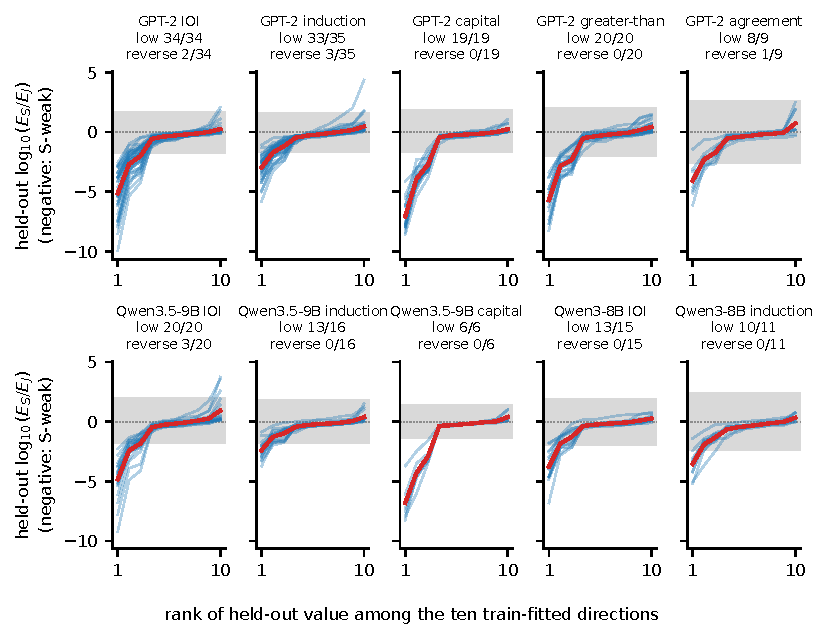
\includegraphics[width=\textwidth]{figures/fig_spectrum.pdf}
\caption{Held-out profiles behind Table~\ref{tab:matched-full}, support-matched protocol (joint family on the single-site $\alpha$ grid, a sparse design). For each capture (thin
blue lines) the ten generalized eigen-directions are fitted on training rows and frozen; the plot shows their held-out
$\log_{10}(E_S/E_J)$ energy ratios \emph{sorted by held-out value} (order statistics). Negative values are S-weak: single-site evidence constrains these hypothesis differences less than joint evidence does.
The low end is the minimum over the ten frozen directions, not the named generator of \S\ref{sec:predict}, and need
not be the first training eigenvector. The thick red line is the mean of the held-out order statistics. The grey band applies the percentiles of
Appendix~\ref{app:protocol} to the same-family nulls of all captures in the cell, pooled, and is shown for display; the
escape counts in the panel titles and in Table~\ref{tab:matched-full} leave each capture's own nulls out, as in
Appendix~\ref{app:protocol}. In GPT-2 $\times$ agreement, a reverse endpoint exceeds its leave-one-capture-out upper bound
while remaining below the displayed upper bound.}
\label{fig:spectrum}
\end{figure}

\begin{figure}[h]
\centering
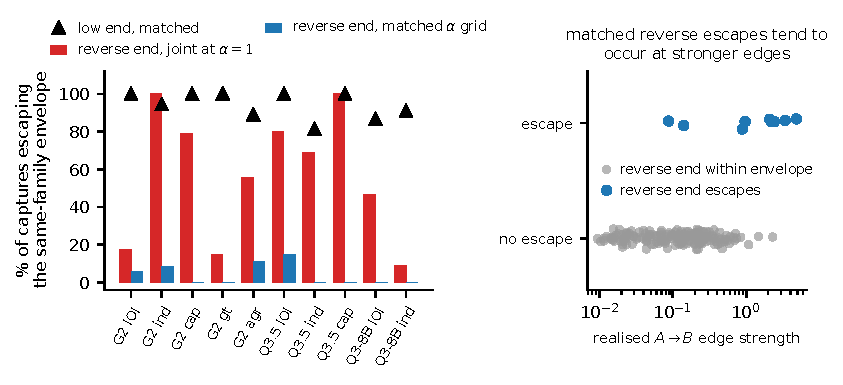
\includegraphics[width=\textwidth]{figures/fig_matched.pdf}
\caption{Support matching and escapes of the same-family envelope. \emph{Left:} percentages of captures whose
optimised profiles escape at the low (S-weak) or reverse (joint-weak) end: red bars, reverse end with the joint family at $\alpha=1$; blue bars, reverse end on
the matched grid; black triangles, low end on the matched grid. Matching reduces reverse escapes.
\emph{Right:} each point is a capture; edge strength (the matched analysis's all-rows statistic, logarithmic axis)
is plotted against the binary matched-protocol reverse-escape indicator, with vertical jitter. Blue points escape at the reverse end;
grey points do not escape at that end, although their low end may escape. Escapes are associated with stronger edges. Tick labels: G2, GPT-2; Q3.5, Qwen3.5-9B-Base; Q3-8B, Qwen3-8B;
ind, induction; cap, capital; gt, greater-than; agr, agreement.}
\label{fig:matched}
\end{figure}

\begin{table}[!htbp]
\centering\small
\begin{tabular}{lcc}
\toprule
model $\times$ task & median $r(g_R)$ & $r(g_R)>10\times$ \\
\midrule
GPT-2 $\times$ IOI          & $\PredGPTIOIRatio$  & \PredGPTIOICount \\
GPT-2 $\times$ induction    & $\PredIndGPTRatio$  & \PredIndGPTCount \\
GPT-2 $\times$ capital      & $\PredCapGPTRatio$  & \PredCapGPTCount \\
GPT-2 $\times$ greater-than & $\PredGtGPTRatio$   & \PredGtGPTCount \\
GPT-2 $\times$ agreement    & $\PredAgrGPTRatio$  & \PredAgrGPTCount \\
Qwen3.5-9B $\times$ IOI     & $\PredQwenIOIRatio$ & \PredQwenIOICount \\
Qwen3.5-9B $\times$ induction & $\PredIndQwenRatio$ & \PredIndQwenCount \\
Qwen3.5-9B $\times$ capital & $\PredCapQwenRatio$ & \PredCapQwenCount \\
\midrule
all                         &                     & \PredTotalCount \\
\bottomrule
\end{tabular}
\caption{Held-out $J/S$ energy ratios of the named generator $g_R$ against the unmatched joint family (raw donors,
$\alpha=1$), repeating its columns of Table~\ref{tab:predict} on the earlier unmatched captures. The qualitative result persists ($\PredTotalCount$ above $10\times$); the magnitude of the $J/S$
ratio depends on the joint support, and the cohorts differ in precision by cell (Appendix~\ref{app:protocol}).}
\label{tab:predict-unmatched}
\end{table}

\paragraph{The named generator and the one-at-a-time baseline.} In the captures, writing $b=ma+c+\varepsilon$ with the recorded
clean $b_0$, the clamped generator equals $m(a-a_0)^2+(a-a_0)(ma_0+c-b_0+\varepsilon)$. Both generators clear $10\times$ in
$\OfatBoth$ captures, $g_R$ alone in $\OfatOnlyRecompute$, $g_C$ alone in $\OfatOnlyClampedCount$, and neither in
$\OfatNeither$, a net difference of $\OfatNetDifference$. The median $r(g_R)$ is $\EdgeBlindWeak$ on weak-edge captures and
$\EdgeBlindStrong$ on the $\EdgeNStrong$ strong-edge ones, of which $\EdgeStrongGtTen$ exceed $10\times$. Of the surviving reverse
escapes of \S\ref{sec:pitfalls}, $\ReverseSurvivorsWeak$ fall below the strong-edge threshold. For the GPT-2 IOI captures, the
single-site range of $a$ exceeds its range under the unmatched joint family by a median factor of $\FigOneBCaptureMedian$,
the support gap behind Figure~\ref{fig:reachable}.

\paragraph{The realised edge, measured.} On all $\EdgeN$ support-matched captures, the absolute Euclidean cosine between the
recompute and clamped generators, in the fixed whitened, column-scaled coefficient basis, falls as the training-row edge strength
$s$ defined in \S\ref{sec:predict} rises (Spearman $\EdgeCosRho$; with the absolute whitened slope it is $\EdgeCosRhoSlope$). Its median is
$\EdgeWeakCos$ below $s=0.10$ and $\EdgeStrongCos$ on the $\EdgeNStrong$ captures at or above it. These cosines are
parameterisation-dependent and descriptive; they do not show that the two designs are equivalent. On the
strong-edge captures the median held-out ratio is $\EdgeStrongSepGC$ for $g_C$ and $\EdgeBlindStrong$ for $g_R$, and
the median within-capture ratio $r(g_R)/r(g_C)$ is $\EdgeStrongRatio$. The design comparison rests on these energy
ratios and on Table~\ref{tab:predict}: the one-at-a-time generator accounts for most threshold exceedances in this
chart, and the recompute generator has an additional advantage on stronger edges.

% ===================================================================== F ====
\clearpage
\section{Chart selection in full}
\label{app:chart}

This experiment compares recompute single-site evidence $R$ with clamped single-site evidence $C$, not single-site
with joint evidence. In the unembedding chart the absolute whitened edge slope is small (median $\RCUchartChartM$), so the
two designs almost coincide and both ends of their optimised profiles are nominally significant in only
$\RCUchartMutual$ cells. We therefore chose the
downstream coordinate by maximising a regularised variance ratio between the arms, using states only; the corresponding
spread ratio is $\mathrm{sd}(b\mid\text{arm }A)/\mathrm{sd}(b\mid\text{arm }B)$. In that chart the edge is strong (median $|m|=\RCChartM$). Scoring the held-out $R/C$ energy profile of the
train-fitted generalized eigen-directions, the recompute-weak end escapes the same-family envelope in $\RCPooledR$
captures, and the clamped-weak end escapes in every retained capture; both ends are nominally significant in
$\RCMutual$ cells.

The chart was fitted on states of the capture on which it was scored. In addition to the readout screen,
this analysis excludes captures with an arm-$A$/arm-$B$ spread ratio above $50$: $\RCDropped$ captures in the
own-chart and donor-holdout analyses. Holding out donors is not enough, because the chart is still fitted on the
capture's own prompt; the recompute-weak end still escapes in $\RCHoldoutPooledR$ captures.

With the chart of a different seed of the same layer pair, the
recompute-weak end escapes in $\RCXseedPooledR$ captures and both ends are nominally significant in $\RCXseedMutual$
cells (GPT-2 capital, GPT-2 IOI and Qwen3.5-9B capital). The cross-seed analysis covers the eight cells with an
available source chart, and its artifact predates the Qwen3-8B cross-seed captures, so the cohorts differ and the
comparison is not a paired effect estimate. For example, GPT-2 induction falls from $\RCGPTIndRblind$ to
$\RCGPTIndXseedRblind$.

A seed change does not partition content either:
$\AuditXseedSamePrompt$ evaluated captures share the chart source's base prompt, and donors are drawn from a shared
pool without a cross-seed exclusion rule. This is a cross-seed transfer control, not a disjoint-content
validation. The reversal between cells under this control is consistent with selection; the differing cohorts limit its interpretation.

The selection criterion is a variance ratio whose denominator is estimated from at most $16$ donor directions in a
much larger space ($768$ dimensions for GPT-2). In the GPT-2 captures for which this was logged, the selected direction had
negligible projection onto the span of the donor directions used to estimate the denominator, so its variance ratio was controlled by the
regulariser. The chart is therefore not ``the direction in which $A$ drives $B$'' but ``the direction in which $A$
drives $B$ and these particular donors do not''.

% ===================================================================== G ====
\section{Two planned hypotheses that failed, and two withdrawn claims}
\label{app:negatives}

Four planned hypotheses did not survive. Two are the withdrawn claims of \S\ref{sec:pitfalls}: (1) mutual
non-domination of single-site and joint evidence (support confound; Appendix~\ref{app:matched}) and (2) mutual
non-domination of recompute and clamped single-site evidence in a chart optimised on the scored states (chart
selection; Appendix~\ref{app:chart}). The other two failed their
criteria. Hypotheses (3) and (4) have dated preregistration records; for (1), registration and results first
enter version control together, so their order cannot be verified; for (2), no dated preregistration entry exists.

\paragraph{(3) Failed hypothesis: a circuit with high in-family faithfulness degrades reciprocally across families.} We fitted and froze
an edge-attribution circuit under each intervention family and scored it under both. The registered gate required
in-family faithfulness of at least $0.85$ and a cross-family drop of at least $0.25$ in both directions. It failed.
The recovered component sets largely overlapped, but overlap alone does not show that transfer cannot degrade. A
circuit is a set of components, whereas the ambiguity studied here lives in functional form, which a set cannot
express.

\paragraph{(4) Failed hypothesis: interpretability representations have distinctive weakly constrained subspaces.} We expected a logit
lens or a tuned lens to show S-weak subspaces distinguishable from matched compression controls. The registered success criterion required an effect outside the matched same-family and
compression nulls, a nontrivial held-out effect, and a consistent direction across multiple model-by-task units.
For $12$ GPT-2 captures in a four-dimensional chart, entries below are capture medians of the held-out energy share
$v_S=E_S/(E_S+E_J)$ of the least-energy training direction. The same-family null is rebuilt at each degree; each null
entry is the capture median of the per-capture $5$th percentile over five same-family resamples at the degree
indicated by its column header.

The arm we call the attention-output unembedding (the row the accepted version labelled ``logit lens''; C57) maps each
last-token attention-module output $A$ to $\rho(A)=\bigl((A-\bar A)/(\operatorname{sd}(A)+10^{-6})\bigr)W_U^{\top}$,
evaluated through its isometric SVD reduction; it uses this custom standardization rather than the model's learned final
LayerNorm and acts on attention outputs, not residual-stream states, so it is not the conventional logit lens. The arm
labelled ``tuned lens'' in the accepted version is a least-squares linear surrogate fitted to this attention-output
unembedding of the first capture's patch-$A$-arm rows and reused across captures and
sites. Of its calibration rows, $\TLCalibOverlap$ fall in that capture's scored half; only the subsequent chart
fit is restricted to training rows.

\begin{center}\small
\begin{tabular}{lrrrr}
\toprule
 & \multicolumn{2}{c}{share $v_S$} & \multicolumn{2}{c}{same-family null ($5$th pct.)} \\
\cmidrule(lr){2-3}\cmidrule(lr){4-5}
representation & $\mathcal F=\mathcal P_{\le1}$ & $\mathcal F=\mathcal P_{\le2}$ & $\mathcal F=\mathcal P_{\le1}$ & $\mathcal F=\mathcal P_{\le2}$ \\
\midrule
raw activations & $\MCRawDegOne$ & $\MCRawDegTwo$ & $\MCRawNull$ & $\MCRawNullTwo$ \\
attention-output unembedding & $\MCLLDegOne$  & $\MCLLDegTwo$  & $\MCLLNull$ & $\MCLLNullTwo$ \\
linear surrogate of it & $\MCTLDegOne$  & $\MCTLDegTwo$  & $\MCTLNull$ & $\MCTLNullTwo$ \\
\midrule
random projection (matched control) & $\MCRandDegOne$ & $\MCRandDegTwo$ & $\MCRandNull$ & $\MCRandNullTwo$ \\
\bottomrule
\end{tabular}
\end{center}

\noindent At degree $1$ each row's capture-median share lies below its degree-1 null by a factor of
$\MCNullRatioOneLo$--$\MCNullRatioOneHi$; at degree $2$ it lies below its degree-2 null by a factor of
$\MCNullRatioTwoLo$--$\MCNullRatioTwoHi$. These factors are ratios of the capture-median null to the capture-median
share, not medians of within-capture ratios. Degree-3 values fall below the numerical resolution of the computation,
where even an orthogonal reparameterisation moves them substantially, so we do not report them.

The captures cover one model-by-task unit (GPT-2, IOI). The compression control is one fixed pair of random site projections reused across
captures rather than a distribution over projections. The captures therefore cannot establish the criterion, which
was not met; this shows neither that representation effects are absent nor that any representation separates. At degree $2$
the attention-output-unembedding share is below the random-projection share in $\MCLLBelowRandTwo$ captures, the raw-activation share in
$\MCRawBelowRandTwo$ and the surrogate's share in $\MCTLBelowRandTwo$; the direction is therefore not specific to the
attention-output unembedding, and these are descriptive comparisons within that one unit. The registration treats cross-representation
eigenvalue magnitudes as class-relative, so between-row differences in the table do not by themselves establish the
registered effect. A sparse-autoencoder arm was omitted by protocol, since no fixed released autoencoder was available
for these models. These results concern the implemented representations and do not establish a general conclusion
about tuned lenses.

% ===================================================================== H ====
\section{Per-cell results and stricter checks}
\label{app:units}

\paragraph{Per-cell results.} Table~\ref{tab:predict} gives, for each model $\times$ task cell, the median held-out $J/S$
energy ratio $r(g_R)$ of the recompute generator $g_R$, the number of captures in which that ratio exceeds $10\times$,
and the same count for the one-at-a-time (clamped) generator $g_C=(a-a_0)(b-b_0)$. Both generators are scored on the same
recompute single-site and joint states, and a large ratio means the direction is S-weak. The $10\times$ threshold is
descriptive. GPT-2 is GPT-2 small; Qwen3.5-9B is Qwen3.5-9B-Base.

\begin{table}[!htbp]
\centering\small
\caption{Held-out $J/S$ energy ratios of the geometry-named direction $g_R$, with the one-at-a-time generator $g_C$ as
baseline, by model $\times$ task cell. Both generators are scored on the same recompute single-site and joint states.
The ratio column gives the median $r(g_R)$; the other columns count captures above $10\times$.}
\label{tab:predict}
\begin{tabular}{lccc}
\toprule
model $\times$ task & median $r(g_R)$ & $r(g_R)>10\times$ & $r(g_C)>10\times$ \\
\midrule
GPT-2 $\times$ IOI                & $\PredGPTIOIMRatio$  & \PredGPTIOIMCount  & \PredGPTIOIMOfat \\
GPT-2 $\times$ induction          & $\PredIndGPTMRatio$  & \PredIndGPTMCount  & \PredIndGPTMOfat \\
GPT-2 $\times$ capital            & $\PredCapGPTMRatio$  & \PredCapGPTMCount  & \PredCapGPTMOfat \\
GPT-2 $\times$ greater-than       & $\PredGtGPTMRatio$   & \PredGtGPTMCount   & \PredGtGPTMOfat \\
GPT-2 $\times$ agreement          & $\PredAgrGPTMRatio$  & \PredAgrGPTMCount  & \PredAgrGPTMOfat \\
Qwen3.5-9B $\times$ IOI           & $\PredQwenIOIMRatio$ & \PredQwenIOIMCount & \PredQwenIOIMOfat \\
Qwen3.5-9B $\times$ induction     & $\PredIndQwenMRatio$ & \PredIndQwenMCount & \PredIndQwenMOfat \\
Qwen3.5-9B $\times$ capital       & $\PredCapQwenMRatio$ & \PredCapQwenMCount & \PredCapQwenMOfat \\
Qwen3-8B $\times$ IOI             & $\PredQIOIMRatio$    & \PredQIOIMCount    & \PredQIOIMOfat \\
Qwen3-8B $\times$ induction       & $\PredQIndMRatio$    & \PredQIndMCount    & \PredQIndMOfat \\
\midrule
all captures                      &                      & \PredMTotalCount   & \OfatRowCount \\
\bottomrule
\end{tabular}
\end{table}

\paragraph{Donor indices.} The row split in \S\ref{sec:predict} places states from the same donor on both
sides, since each donor contributes $\NAlpha$ coefficients. Under a common partition of donor indices that scores a joint row only if both of its
donor indices are held out, $g_R$ exceeds $10\times$ in $\DonorNamedCount$ captures and $g_C$ in $\OfatDonorCount$
(both $\OfatDonorBoth$, only $g_R$ $\OfatDonorOnlyRecompute$, only $g_C$ $\OfatDonorOnlyClampedCount$, neither
$\OfatDonorNeither$). This partition holds out donor indices, not donor content: in $\AuditDonorDupCaptures$ captures a
held-out donor's patch-$A$ trajectory is identical to a training donor's, and whether the donor prompts coincide was
not checked. It is therefore not a disjoint-content validation.

\paragraph{Prompt groups.} The $\MatchedN$ captures rest on $\HeldoutPrompts$ (cell, prompt) groups that share clean
activations, donor pools and task instances, because a capture's seed selects its prompt. Counting a group only if \emph{every} capture in it exceeds
$10\times$ under the row split, $g_R$ succeeds in $\HeldoutPromptStrict$ groups and $g_C$ in $\OfatPromptStrict$.
Resampling the groups with replacement, the $2.5$th percentile of the pooled fraction of captures with
$r(g_R)>10$ under the row split is $\HeldoutPromptBootLo\%$. Groups still share models and tasks.

\paragraph{Random directions.} For $200$ Gaussian directions per capture in the training-scaled coefficient basis, the
cell medians of the capture-specific $95$th percentiles range from $\HeldoutNullLo$ to $\HeldoutNullHi$, and $g_R$
exceeds its own capture's $95$th percentile in $\HeldoutBeatsNull$ captures (Appendix~\ref{app:corrections}, C02).

% ===================================================================== I ====
\section{Three sites in a trained model}
\label{app:three}

\paragraph{Design.} Proposition~\ref{prop:ksite} counts rank on the population reachable set. Here we extend the
trained-model energy comparison to three GPT-2 attention blocks: three single-site arms, each site patched alone across the same
coefficient grid with the other two left to the network, against a support-matched joint family over donor triples,
in float32, with the same chart, split and envelope. The layer triples are $5$--$7$--$9$, $5$--$8$--$11$,
$6$--$9$--$11$ and $7$--$9$--$11$, with three seeds each.

\paragraph{Full rank, weakly constrained directions.} The design matrices have full numerical rank (singular-value
tolerance $10^{-9}$) under both families, so the comparison concerns ill-conditioning. The profile reports
single-site/joint energy, so more negative log ratios mean weaker single-site evidence. For each capture we score every
frozen training eigenvector and take the minimum held-out log energy ratio $\log_{10}(E_S^{\mathrm{te}}/E_J^{\mathrm{te}})$. In the
$\ThreeDegThreeDim$-dimensional degree-3 class the median over captures of these minima is $-\ThreeDegThreeLogRatio$;
the profile minimum escapes the same-family envelope in $\ThreeDegThreeSblind$ captures and the profile maximum in
$\ThreeDegThreeReverse$. At degree $2$ ($\ThreeDegTwoDim$ dimensions) the corresponding median is
$-\ThreeDegTwoLogRatio$, and the profile minimum escapes in $\ThreeDegTwoSblind$.

% ===================================================================== J ====
\section{Legacy robustness checks and a synthetic check of the estimator}
\label{app:robust}

\paragraph{Charts and classes.} These are exploratory legacy checks on the earlier unmatched captures. They use a
Euclidean ridge $G_Q+10^{-10}I$ rather than the covariant pencil, and whitening and feature scaling estimated on all
rows; the data-derived charts and the non-polynomial classes therefore also use evaluation states. Only the
eigensolve is fitted on the training half, so these are not held-out validations in the sense of
\S\ref{sec:practical}. Both tables report the median evaluation-half $J/S$ ratio of the least-energy direction.

\begin{center}\small
\begin{tabular}{lr}
\toprule
chart (eight GPT-2 captures) & median $J/S$ ratio, legacy procedure \\
\midrule
$u$ (unembedding difference) & $\CoordUSblind$ \\
top activation principal component & $\CoordPConeSblind$ \\
pooled intervention mean $-$ clean & $\CoordDiffSblind$ \\
four-dimensional chart (two components per site; degree $2$) & $\CoordPCtwodSblind$ \\
\bottomrule
\end{tabular}
\end{center}

\begin{center}\small
\begin{tabular}{lrr}
\toprule
class & GPT-2 ($12$ captures) & Qwen3.5-9B ($15$ captures) \\
\midrule
polynomial & $\BGPTPolySblind$ & $\BQwenPolySblind$ \\
fixed-grid radial basis (RBF; different class) & $\BGPTRbfSblind$ & $\BQwenRbfSblind$ \\
random Fourier (different class) & $\BGPTFourierSblind$ & $\BQwenFourierSblind$ \\
\bottomrule
\end{tabular}
\end{center}

\noindent The submitted version also reported a Taylor row as an invariance check. It was built with a zero centre,
i.e.\ the identical design matrix, so its exact agreement with the polynomial row is not a check, and it is removed
(Appendix~\ref{app:corrections}, C39). Magnitudes differ across classes, as Definition~\ref{def:blind} predicts, and
we never compare them as though the classes shared a geometry.

\paragraph{A synthetic check of subspace membership.} In synthetic union-of-slices data with a planted generator $g$,
the pencil estimator's least-energy direction lies close to the known degree-3 blind subspace
$\operatorname{span}\{g,ag,bg\}$ in a fixed coefficient basis: its Euclidean projection residual is $\PCResidZero$ at zero noise and at most
$\PCResidWorst$ up to noise $10^{-1}$, against a random-vector $1$st percentile of at least $\PCRandPOne$. This checks
subspace membership, not recovery of a unique generator, and it is basis-dependent.

% ===================================================================== K ====
\section{Non-invariant checks and worst-case bounds}
\label{app:noninvariant}

\paragraph{Covariant pencil.} Under $\varphi\mapsto L\varphi$ every term of the pencil of \S\ref{sec:practical} transforms as
$L(\cdot)L^\top$, so its spectrum is invariant in exact arithmetic. In a numerical check of the unregularised pencil on
the earlier unmatched captures, the largest cell median of the per-capture maximum relative eigenvalue change under a
reparameterisation is $\ReparamInvariance$. A Euclidean ridge on $G_Q$ and Euclidean coefficient angles or cosines are
not invariant; they are used only in Appendices~\ref{app:matched}, \ref{app:robust} and~\ref{app:noninvariant}, as
descriptive, legacy or non-invariance checks.

\paragraph{Euclidean ridge.} $G_Q+\lambda I$ does not transform covariantly under $\varphi\mapsto L\varphi$ for
non-orthogonal $L$. Under a reparameterisation of condition number $50$ on the Qwen3.5-9B IOI captures, the
$\lambda=10^{-6}$ spectrum moves by a median relative $\EucRegInvariance$, against $\CovRegInvariance$ for the covariant
regulariser of \S\ref{sec:practical}.

\paragraph{Principal angles.} Euclidean angles between coefficient subspaces depend on the parameterisation of the
coefficient space. On the earlier unmatched captures, the principal angles between the low-energy eigenspaces of the single-site and
joint training Grams have a median of $\AngleBefore^\circ$. Recomputing both eigenspaces after a random
reparameterisation of the same condition number gives $\AngleAfter^\circ$. Both summaries are medians over model--task
cells of within-cell medians of per-capture median angles. We report no principal-angle quantity as evidence; the submitted version used such angles as a
stability check, and they are removed (Appendix~\ref{app:corrections}, C34).

\paragraph{Worst-case spectral bounds are vacuous here.} Treating the finite intervention grid as a population, a
matrix Bernstein inequality \citep{tropp2015introduction} bounds $\|\widehat G_Q-G_Q\|$; for a two-sided deviation of a
Hermitian sum the intrinsic-dimension version carries a factor $8\,\mathrm{intdim}$ and holds only above a threshold
deviation (C15). The Davis--Kahan bound \citep{yu2015davis} then limits $\|\sin\Theta\|_F$ for the bottom-$k$
eigenspace ($k=3$) by $2\sqrt k\,\|\widehat G-G\|/\gamma_k$, where $\gamma_k=\lambda_{k+1}-\lambda_k$ in increasing
order. For the joint family the median relative gap at that boundary is $\FSGPTEigengapBottomRel$ (GPT-2) and
$\FSQwenEigengapBottomRel$ (Qwen3.5-9B). The submitted version took the gap at the top of the spectrum and used the
understated constant, and both corrections enlarge the bound, so it is vacuous a fortiori; its numerical bounds are
withdrawn (C38). The measured log--log concentration slopes of the single-site family, $\FSGPTRateSlope$ and
$\FSQwenRateSlope$ against a theoretical $-0.5$, are consistent with the rate but span under one decade of $n$.
Nothing here is used as a guarantee.

\paragraph{Held-out energies are not certificates.} For a direction frozen on training rows,
$v^\top\widehat G_{\mathrm{test}}v$ is an out-of-fit mean over the complementary rows and needs no eigengap.
The usual certificate conditions on training rows and applies a fixed-vector concentration inequality to an
independent test sample. It is not directly available here: test rows are the deterministic complement of training
rows in a fixed finite grid. We make no certification claim.

% ===================================================================== L ====
\section{IOI analysis in detail}
\label{app:ioi}

\begin{table}[t]
\centering\small
\caption{Fit, prediction, Wald envelopes and coverage of the working model on the published IOI head pairs
\status{exploratory; three base prompts; $\MisN$
captures}. Compare the prediction errors with predicting zero, and the envelope widths with their coverage. $R^2$ rows: median over ten donor partitions of the median over captures; ``additive terms only'' is a
separate additive-only refit. Contrast rows use donor partition seed $0$; RMS entries are medians over captures. Predicting $0$ has an error
equal to the RMS of the executed $T_C$ over these held-out joint rows, a subset of the states behind the median RMS
in the text.
For held-out prediction, fits use only rows whose donors are all training donors; a joint row is scored only when both its donors are held out.
``Worse than $0$'' counts captures whose nominal $95\%$ donor-bootstrap interval for the excess error over predicting
zero lies above zero (fits held fixed). A \emph{Wald envelope} is, per capture, the median over the $256$ joint states
of the largest $|T_C|$ inside the fit's $95\%$ Wald region for $\gamma$ (point estimate plus radius, all rows of the
family); envelope entries are medians over captures, with the percentage taken per capture. It is a working-model
identification width that reflects the design, the misspecified fit and its residual variance, not an observed error
or a bound on the network. Coverage counts captures in which, at every joint state, the executed $|T_C|$ lies inside
that state's envelope.}
\label{tab:scales}
\begin{tabular}{lcc}
\toprule
 & single-site fit & joint fit \\
\midrule
held-out $R^2$ on joint readouts, full cubic & $\RespSJR$ & $\RespFullThreeJJ$ \\
held-out $R^2$ on joint readouts, additive terms only & $\RespAddThreeSJ$ & $\RespAddThreeJJ$ \\
held-out RMS error predicting $T_C$, logits (predicting $0$: $\MfZero$) & $\MfSThree$ & $\MfJThree$ \\
fits predicting $T_C$ worse than $0$ & $\MfSWorse$ & $\MfJWorse$ \\
Wald envelope, logits & $\AdqEnvS$ & $\AdqEnvJ$ \\
Wald envelope, \% of B-arm swing & $\MisS$ & $\MisJ$ \\
coverage of the executed $|T_C|$ & $\AdqCoverUpperS$ & $\AdqCoverUpperJ$ \\
\bottomrule
\end{tabular}
\end{table}

\paragraph{Design details.} The published pairs combine the S-Inhibition heads 7.3, 7.9, 8.6 and 8.10 with the Name Movers 9.6, 9.9
and 10.0. The control pairs combine the early heads 0.5, 1.2, 2.9 and 3.4, which have no claimed IOI role, with the same Name
Movers.

\paragraph{The executed contrast in detail.} Across the captures on the three base prompts, the interquartile range of
the RMS of $T_C$ is $\AdqRmsTLo$--$\AdqRmsTHi$ logits. Normalising each capture's RMS by its mean absolute per-donor effect at
$\alpha\approx1$ (median $\AdqEffectAlphaOne$ logits) gives a median percentage of $\AdqRmsTPctEffect\%$.
The largest single $|T_C|$ in a capture is a median $\AdqMaxTPctEffect\%$ of that effect, and $\MfMaxAbsMax$ logits at most.

\paragraph{The working model in detail.} The median edge $R^2$ of the fitted edge is $\QCEdgeRTwo$, so single-site data
inform the cross coefficients only through departures from the affine edge; the low edge $R^2$ does not by itself show that the scatter is small, and the relevant scale comparison is the ratio $\GrpIOIEdge$ of the standard deviation of $b$ on the patch-$A$ arm to that on the patch-$B$ arm. The design gap, whose median in the shared chart is $\QCInfoRatio$, is $\QCInfoRatioOwnChart$ if each family is
standardised separately. The single-site cubic's held-out $R^2$ on joint readouts is negative in at least
$\RespSJNegMin$ of $\MisN$ captures under each of ten donor partitions. For the detection analysis, the ratio of arm-$A$
to arm-$B$ residual variance is a median $\DetArmVarIOI$ for published heads and $\DetArmVarCtrl$ for controls, which
contradicts the equal-variance assumption of the pooled covariance.

\paragraph{Covariance sensitivity and the joint test.} Under a pooled covariance, single-site evidence rejects $\gamma=0$ in
$\QCRejS$ published captures against $\QCCtrlRejS$ controls. Under five alternative covariances controls reject in
$\DetCtrlRobLo$--$\DetCtrlRobHi$ of $\QCCtrlN$ and published heads in $\DetIOIRobLo$--$\DetIOIRobHi$ of $\QCN$. These are
covariance-sensitivity calculations for a misspecified model, not a validated calibration. The replication shows the same
sensitivity to the covariance estimator (Appendix~\ref{app:replication}). The joint fit, with the marginal-sum donor covariance
$V_{\mathrm{up}}+V_{\mathrm{down}}$ (which omits the intersection term and cross-role donor dependence; its calibration is
unknown), rejects in $\DetIOIJTwo$ published and $\DetCtrlJTwo$ control captures.

\paragraph{Estimands of the two tests.} The single-site and joint tests of \S\ref{sec:ioi} need not target the same
coefficients. Correct specification of the cubic model on both supports guarantees a common $\gamma$. With the
misspecification shown in Table~\ref{tab:scales}, each fit instead approximates the network on its own support: near the
two arms for single-site evidence and over the filled region for joint evidence. Sharing a chart therefore does not
guarantee a common estimand. With the pooled working-model covariance $V_S+V_J$, the single-site estimate $\gamma_S$ is
inconsistent with the joint estimate $\gamma_J$ in $\DetInconsistent$ single-site rejections ($\DetInconsistentAll$
overall), and the joint test's nominal plug-in power at $\gamma_S$ rounds to $\DetPowerMin$: had $\gamma_S$ been the joint
fit's target, the joint test would almost always have rejected.

\paragraph{Relation to the submitted version.} The Wald-envelope percentages here replace the submitted version's, which
evaluated two of the four terms of the contrast and named the wrong denominator (Appendix~\ref{app:corrections},
C05--C07).

\paragraph{Working-model identification widths.} The widths (computed from nominal Wald regions) of single-site working-model fits vary with degree, covariance and prompt.
Percentages are medians over captures (all $\MisN$ published captures, or those of one prompt where stated)
of each capture's single-site envelope divided by its B-arm swing and expressed as a percentage. By degree: $\EnvSDtwo$ (degree $2$), $\MisS$ ($3$), $\EnvSDfour$ ($4$); the single-site
envelope exceeds the joint one in every capture at every degree, and the smallest ratio of medians over degrees is
$\EnvRatioMin$. By covariance at degree $3$: pooled $\MisS$, HC0 (heteroskedasticity-consistent) $\AdqEnvSHCzero$,
donor-clustered $\AdqEnvSCluster$. By prompt: $\AdqSeedZeroEnvS$, $\AdqSeedOneEnvS$ and $\AdqSeedTwoEnvS$; the
single-site envelope exceeds the whole swing in $\AdqSeedZeroOverOne$, $\AdqSeedOneOverOne$ and $\AdqSeedTwoOverOne$
captures of the three prompts.

Each pointwise envelope is the sum of a centre $|D^\top\hat\gamma|$ and a Wald radius. Taking medians over
joint states and then captures gives centres of $\AdqCentreS$ logits single-site and $\AdqCentreJ$ joint,
and radii of $\AdqRadiusS$ and $\AdqRadiusJ$ logits, respectively. Coverage of the executed $|T_C|$
at all $256$ joint states, under $|T_C|\le|D^\top\hat\gamma|+\text{radius}$: single-site $\AdqCoverUpperSTwo$,
$\AdqCoverUpperS$, $\AdqCoverUpperSFour$ at degrees $2$--$4$; joint $\AdqCoverUpperJTwo$, $\AdqCoverUpperJ$,
$\AdqCoverUpperJFour$. Under $|T_C-D^\top\hat\gamma|\le\text{radius}$: single-site $\AdqCoverIntervalS$ and joint
$\AdqCoverIntervalJ$ at degree $3$. The B-arm swing is a median $\AdqSwingOverEffect$ times the mean absolute per-donor
effect at $\alpha\approx1$.

\paragraph{Controls.} Control head pairs share the Name Movers, prompts and donors with the published pairs. The
exploratory captures did not measure the numerical floor, and the replication did not resolve the control family
under the registered floor rule (Appendix~\ref{app:replication}), so these data support no published/control
transport ratio and no above-control conclusion. Between-prompt and within-prompt standard deviations of $\log$ RMS
$T_C$ were $\AdqSdBetweenPrompt$ and $\AdqSdWithinPrompt$; they informed the replication design.

\paragraph{The edge in the query chart.} In this appendix and in \S\ref{sec:ioi}, the edge strength $s$ of \S\ref{sec:predict} is computed on all single-site rows of a capture, not only on training rows. The median edge
strength of the published pairs is $\QCEdgeVsCtrl\times$ that of the control pairs (ratio of capture medians). With source heads as units, the four published and four control heads separate completely
(exact one-sided Mann--Whitney $p=\HeadEdgeExactP$, the smallest attainable). Each head's value first averages
$\log_{10}s$ over prompts whose capture passed the screen, then over its Name Movers. This is a descriptive
conditional permutation summary, since the heads share Name Movers, prompts and the model. It is
consistent with query mediation and is not a test of it.

\paragraph{Head groups, with heads as units.} We repeat the procedure on previous-token $\to$ induction heads and on
the control group. Induction heads read previous-token information through keys; the final-position query chart and final-position patch do not test that
mechanism, so this group is a comparison of designs, not a second query-mediated circuit. The median edge strength is $\GrpIOIEdge$ for the published IOI pairs, $\GrpIndEdge$ for the
induction group and $\GrpCtrlEdge$ for controls, and the design gap runs the other way: $\GrpIOIInfoRatio$,
$\GrpIndInfoRatio$ and $\GrpCtrlInfoRatio$. The gap is largest for the controls, whose edge is flattest, so it is a
property of the design, not evidence about IOI; the association is largely structural, because a small patch-$A$
spread of $b$ reduces single-site cross-term information. With source heads as units ($n=\HeadRhoN$), the rank
correlation between edge and gap is $\HeadRho$ (exact permutation $p=\HeadRhoP$ one-sided, $\HeadRhoPTwo$ two-sided), a
descriptive conditional permutation summary, since heads share target heads, prompts and the model; the submitted
version's configuration-level $p$-values treated captures that share heads and prompts as independent. For the induction group,
single-site evidence rejects $\gamma=0$ in $\AdqIndRejSHomo$ captures under a pooled covariance and in
$\AdqIndRejSLo$--$\AdqIndRejSHi$ of $\GrpIndN$ under the alternative covariances; the marginal-sum joint test rejects in
$\AdqIndRejJTwo$. 

Table~\ref{tab:ident} returns to the unembedding chart for the eight GPT-2 and Qwen3.5-9B cells,
reporting design information for the cross coefficients.

\begin{table}[!htbp]
\centering\small
\begin{tabular}{lccccc}
\toprule
model $\times$ task & design info., $S$ & design info., $J$ & SE ratio $S/J$ & flip rate $S$ & flip rate $J$ \\
\midrule
GPT-2 $\times$ IOI          & $\IdGPTIOIInfoS$  & $\IdGPTIOIInfoJ$  & $\IdGPTIOISeRatio$  & $\IdGPTIOIFlipS$  & $\IdGPTIOIFlipJ$ \\
GPT-2 $\times$ induction    & $\IdGPTIndInfoS$  & $\IdGPTIndInfoJ$  & $\IdGPTIndSeRatio$  & $\IdGPTIndFlipS$  & $\IdGPTIndFlipJ$ \\
GPT-2 $\times$ capital      & $\IdGPTCapInfoS$  & $\IdGPTCapInfoJ$  & $\IdGPTCapSeRatio$  & $\IdGPTCapFlipS$  & $\IdGPTCapFlipJ$ \\
GPT-2 $\times$ greater-than & $\IdGPTGtInfoS$   & $\IdGPTGtInfoJ$   & $\IdGPTGtSeRatio$   & $\IdGPTGtFlipS$   & $\IdGPTGtFlipJ$ \\
GPT-2 $\times$ agreement    & $\IdGPTAgrInfoS$  & $\IdGPTAgrInfoJ$  & $\IdGPTAgrSeRatio$  & $\IdGPTAgrFlipS$  & $\IdGPTAgrFlipJ$ \\
Qwen3.5-9B $\times$ IOI     & $\IdQwenIOIInfoS$ & $\IdQwenIOIInfoJ$ & $\IdQwenIOISeRatio$ & $\IdQwenIOIFlipS$ & $\IdQwenIOIFlipJ$ \\
Qwen3.5-9B $\times$ induction & $\IdQwenIndInfoS$ & $\IdQwenIndInfoJ$ & $\IdQwenIndSeRatio$ & $\IdQwenIndFlipS$ & $\IdQwenIndFlipJ$ \\
Qwen3.5-9B $\times$ capital & $\IdQwenCapInfoS$ & $\IdQwenCapInfoJ$ & $\IdQwenCapSeRatio$ & $\IdQwenCapFlipS$ & $\IdQwenCapFlipJ$ \\
\bottomrule
\end{tabular}
\caption{Identification of the cross coefficients in the unembedding chart, support-matched captures; entries are
medians over captures. \emph{Design info.} is the smallest eigenvalue of the per-observation residualised design Gram
of the cross block given the additive block: a property of the design, not Fisher information about the network.
The standard-error (SE) ratio is $\|\sqrt{\operatorname{diag}V_S}\|_2/\|\sqrt{\operatorname{diag}V_J}\|_2$,
the ratio of the Euclidean norms of the marginal standard-error vectors in this chart. The flip rate
is the fraction of $40$ random complementary row-half splits on which the fitted $ab$ coefficient changes sign; it is
descriptive and parameterisation-dependent.}
\label{tab:ident}
\end{table}

% ===================================================================== M ====
\clearpage
\section{Related work in full}
\label{app:related}

\paragraph{Algebraic experimental design.} For a finite design, $I(R_Q)$ is the design ideal and the rank of the
evidence map is the Hilbert function of the quotient; aliasing is exactly $N(Q,\mathcal P_{\le d})$. This calculus is
due to \citet{pistone1996groebner}, developed in \citet{pistone2001algebraic} and surveyed by
\citet{maruri2012algebraic}. The algebra is inherited from these works. Our contribution is the modelling step: under patch-and-recompute the network,
not the analyst, produces the design points, which makes $R_Q$ a measurable property of a trained model. Recent work
asks interpretability claims to state their intervention class and identification assumptions
\citep{joshi2026causality,lin2026disclose}.

\paragraph{Comparison of experiments, and one-at-a-time designs.} Ordering experiments by informativeness is due to
\citet{blackwell1953equivalent}. For Gaussian linear experiments with known nonsingular noise covariances and a common
mean parameter, Blackwell informativeness is equivalent to Loewner order of the information matrices
\citep{hansen1974comparison}, and \citet{pukelsheim2006optimal} develops the design theory of Loewner-incomparable
pairs. Our resolving preorder coarsens that order to compare only which directions are resolved within $\mathcal F$. Single-site patching
under clamping is a one-at-a-time design, whose inability to estimate interactions is textbook material
\citep{czitrom1999ofat}; the recompute semantics differ from it only through the realised edge (\S\ref{sec:predict}).

\paragraph{Causal mediation.} Patch-and-recompute measures a total effect; clamping measures a controlled direct effect.
Mediation analysis states the assumptions under which each is identified
\citep{pearl2001direct,robins1992identifiability,vanderweele2015explanation}.
\citet{vanderweele2014fourway} gives the decomposition that separates mediation from interaction. \citet{vig2020gender} brought mediation analysis to
language models. \citet{kekic2025joint} identify joint mean effects from observational and single-variable
interventional distributions under a pairwise-confounded additive structural model and equal action supports across
regimes. Our range checks and executed contrasts diagnose related obstacles but do not establish those hypotheses.
\citet{vaidyanathan2026curse} decompose the patching estimand and expose hidden mediator interactions; that concerns
one chosen intervention's effect, not a family's resolving power.

\paragraph{Mechanistic interpretability.} We ask what a body of intervention evidence can resolve.
\citet{meloux2025everything} establish that mechanistic explanations are not unique, and
\citet{venkatesh2026steering} exhibit large equivalence classes of steering vectors. On intervention semantics,
\citet{makelov2024illusion} show that subspace patching can act through dormant pathways. \citet{geiger2025causal}
supply a general language for describing interventions, and \citet{eslami2026acif} studies separating intervention
families for structural causal models. Positive guarantees address other targets: \citet{asiaee2026cif} certifies a
chosen estimand under a stated intervention distribution, and \citet{dhor2026spectral} prove identifiability for a
model-intrinsic spectral primitive, asking what property of the model is recoverable. 

Complementary evaluations concern intervention success and circuit variability.
\citet{bhalla2025unifying} compare interpretability tools by intervention success; \citet{mueller2025mib} benchmark circuit discovery.
\citet{bayatmakou2026many} and \citet{venkatesh2026architecture} study how recovered circuits vary with inputs,
granularity and architecture. 

Our analysis concerns the intervention families used by automated circuit discovery
\citep{conmy2023acdc} and alignment search \citep{geiger2024das}.
Experimental design for choosing interventions \citep{tigas2022interventions} is the constructive counterpart of our negative statement.
Our protocol follows the patching-practice literature
\citep{zhang2024patching,heimersheim2024patching,goldowskydill2023pathpatching}. Self-repair after ablation \citep{mcgrath2023hydra} and the gap between localisation and editing
\citep{hase2023localization} concern what a successful intervention licenses rather than what a family excludes. The
tasks are those of \citet{wang2022ioi}, \citet{olsson2022induction}, \citet{hanna2023greater}, \citet{meng2022locating}
and \citet{finlayson2021causal}.

% ===================================================================== N ====
\section{Reproducibility and use of AI tools}
\label{app:repro}

A claim ledger supplies the reported numerical results and records each number's source artifacts by hash, unit
and aggregation. Verification re-derives the recorded numerical results from the stored artifacts and compares their formatted
values and artifact hashes. Appendix~\ref{app:corrections} is generated separately from the correction ledger, which records an
independent verification check for each entry; associated review files record the adversarial verdicts. The scope and
interpretation of each result are checked separately.

The reproducibility package at \url{https://github.com/Ankush-kadu/activation-patching-identifiability} contains the analysis code, the intervention captures including the replication's, the claim ledger, the preregistration with its frozen hashes, the correction ledger and the manuscript sources. Verifying the claims and
rebuilding the paper need only a CPU; re-collecting captures needs a GPU. Two summary artifacts of the submitted version had no generating script (the mediator-interaction comparison and the path-patching controls); the
corresponding appendix sections are removed.

Large language models assisted with code, protocol drafting, algebraic checking, adversarial review, writing and
literature search. Reported measurements come from executed model interventions and from analyses of stored
artifacts, not from numerical values supplied in model responses. Numerical results and algebraic claims were checked with the archived verification procedures.
The authors reviewed the content and take responsibility for it.

% ===================================================================== O ====
\section{Preregistered replication of the IOI transport analysis}
\label{app:replication}

\paragraph{Registration.} The preregistration, the prompt pool, the collection driver and the analysis script were
frozen by hash, with an empty sealed output directory, before any fresh forward pass. The analysis ran as
registered, with no change after the first data were seen.

\paragraph{Design.} GPT-2 small in float32, with the unchanged collector of \S\ref{sec:ioi}. The $\RepTemplates$ IOI templates of \citet{wang2022ioi} each have a first clause differing from every template
used in this paper's previously inspected captures. We converted them to the name order of our captures and drew
three prompts per template from fixed seeds, giving $\RepPrompts$ prompts. Each prompt has the $12$ published and $12$ control head pairs of
\S\ref{sec:ioi} and the same per-capture design (single-site arms, clamped arm, $256$ joint states), $\RepCaptures$
captures in all. The eight templates are the complete evaluation set and the unit of inference; we report finite-set
criteria over them, not population $p$-values.

\paragraph{Summaries.} For each capture let $r_c$ be the RMS of $T_C$ over the tested joint states and
$q_c=100\,r_c/\text{swing}_c$, where $\text{swing}_c$ is that capture's B-arm readout range.
For prompt $p$, $M_p$ and $M_p^{\mathrm{rel}}$ are the medians of $r_c$ and $q_c$ over its screened published captures;
for template $t$, $V_t$ and $V_t^{\mathrm{rel}}$ are the medians of $M_p$ and $M_p^{\mathrm{rel}}$ over its three prompts.

\begin{center}\small
\begin{tabular}{lcccccccc}
\toprule
template & T1 & T2 & T3 & T4 & T5 & T6 & T7 & T8 \\
\midrule
$V_t$ (logits) & $\RepVTOne$ & $\RepVTTwo$ & $\RepVTThree$ & $\RepVTFour$ & $\RepVTFive$ & $\RepVTSix$ & $\RepVTSeven$ & $\RepVTEight$ \\
$V_t^{\mathrm{rel}}$ (\%) & $\RepVrelTOne$ & $\RepVrelTTwo$ & $\RepVrelTThree$ & $\RepVrelTFour$ & $\RepVrelTFive$ & $\RepVrelTSix$ & $\RepVrelTSeven$ & $\RepVrelTEight$ \\
\bottomrule
\end{tabular}
\end{center}

\paragraph{Validity gates.}
\begin{description}[leftmargin=1.2em,itemsep=1pt,topsep=1pt,parsep=0pt,font=\normalfont]
\item[(V1)] Re-collecting all $24$ captures of an original seed had to reproduce the stored
readouts to within $10^{-4}$ logits and the state coordinates to a relative $10^{-5}$, with equivalent re-execution
under the original batching; all matched exactly.
\item[(V2)] The single-site, clamped and joint rows were re-executed in
reverse order with batch size $7$ instead of $16$, keeping donor activations and the clean pass fixed; a capture's floor
is the RMS of the resulting change in $T_C$, and a family counts as resolved if at least $90\%$ of its captures exceed
ten times their floor.
\item[(V3)] Identity checks: the joint and clamped arms share upstream coordinates, the joint and $B$
arms share downstream coordinates, and pinned coordinates do not move.
\item[(V4)] At least half of the published captures
and at least five templates remain analysable; $\RepScreenedOut$ captures failed the screen, $\RepErrors$ raised errors,
and all eight templates were analysable.
\item[(V5)] Captures with a B-arm swing below $\MfSwingThr$ logits are excluded and
reported; none was.
\end{description}

\paragraph{Registered criteria and outcomes.} H1\textsubscript{abs} passed: $V_t<\MfMargin$ logits was required in
at least $7$ of $8$ templates and observed in $\RepHAbsCount$ (median $\RepVMed$; range $\RepVMin$--$\RepVMax$).
H1\textsubscript{rel} passed: $V_t^{\mathrm{rel}}<1\%$ was required in at least $7$ of $8$ and observed in $\RepHRelCount$ (median $\RepVrelMed\%$; range $\RepVrelMin$--$\RepVrelMax\%$). Both margins were fixed after the exploratory analysis and
are disclosed as such.

H2 assesses the published/control comparison, grouping screened captures by prompt $p$ and Name Mover $n$. In a group with both families present and a positive
control median, $d_{p,n}$ is the log of the median published $r_c$ minus the log of the median control $r_c$; $d_p$ is
the median of the defined $d_{p,n}$ over the prompt's groups and $d_t$ the median of the defined $d_p$ over the
template's prompts. H2 requires $d_t>0$ in at least $7$ of $8$ templates, a positive median of $d_t$, and both
families resolved under V2; a template without a defined $d_t$ does not count. Published contrasts were resolved in $\RepPubResolved$
captures (median RMS $\RepPubRmsMed$ logits; median floor $\RepFloorMed$) but control contrasts in only $\RepCtlResolved$
(median RMS $\RepCtlRmsMed$; median floor $\RepFloorMedCtl$). Under the registered floor rule H2 is floor-limited: we
report no published/control ratio and no above-control finding. The registered decision rule upgrades the section
only if every criterion passes, so the transport result stays exploratory with its smallness replicated as
registered.

\paragraph{Secondary, descriptive.} Across screened published captures, $q_c$ has maximum $\RepPubRelMax\%$ and 90th
percentile $\RepPubRelPninety\%$; these summarise the RMS over the joint states, not the largest $|T_C|$ at a single
state.

The single-site cubic's held-out prediction error for $T_C$ exceeds that of predicting zero in
$\RepSSixWorse$ published captures, by point error. Single-site and joint Wald envelopes cover the executed $|T_C|$ at all joint states
in $\RepSSevenS$ and $\RepSSevenJ$ published captures. Single-site evidence rejects $\gamma=0$ in $\RepPubHomo$ published
and $\RepCtlHomo$ control captures under a pooled covariance, while controls reject in $\RepCtlRobLo$--$\RepCtlRobHi$ of
$\RepCtlN$ under the alternative covariances; $\gamma_S$ is inconsistent with $\gamma_J$ in $\RepInconsistent$ published
captures. The descriptive sensitivity analyses give the same classifications when excluding the template flagged in the registration
for sharing the phrase ``went to'' with an inspected template (T7), or when dropping the screen. These analyses do not
change the registered decisions.

\section{Limitations, status terms and details moved from the main text}
\label{app:limits}

\paragraph{Status terms of Table~\ref{tab:status}.} \emph{Proved}: a theorem on the analysed
slices. \emph{Exact}: a model-free consequence of which states were executed. \emph{Empirical}: a re-analysis of
captures inspected before these analyses were fixed. \emph{Exploratory}: an analysis chosen after the reviews. \emph{Replicated}: a registered criterion met in the preregistered replication. \emph{Floor-limited}: the
registered comparison is unresolved because control contrasts are not resolved above numerical precision.
\emph{Failed}: a planned hypothesis whose criterion was not met. \emph{Withdrawn}: retracted, either already in the
submitted version (marked $^{\dagger}$) or here.

\paragraph{Limitations in full.}
\begin{itemize}[leftmargin=1.2em,itemsep=1pt,topsep=2pt,parsep=0pt]
\item \textbf{Level.} The exact theorems apply only to the analysed operator slices and polynomial single-site arms,
under their stated coordinates and assumptions (Remark~\ref{rem:scope}, Proposition~\ref{prop:ksite}). The
trained-model results concern weak identification in the evaluated charts and classes, not exact non-identifiability;
the clamped family's polynomial kernel is structural.
\item \textbf{Class and chart.} $N(Q,\mathcal F)$ depends on $\mathcal F$ and the chart by construction, so the
framework requires a declared protocol and gives no context-free result.
\item \textbf{Scope and selection.} The trained-model geometry analyses use $\MatchedN$ two-site captures across $\PredCells$
model--task cells. Captures share prompts and tasks, the joint design is sparse rather than an exact product-support
match, and the readout screen conditions the analysed sample. Counts are therefore descriptive, and we make no
population claim.
\item \textbf{Named direction.} The analysis reuses previously inspected captures, and the one-at-a-time baseline
explains most threshold exceedances.
\item \textbf{IOI.} The study covers GPT-2 small and one published edge class. The executed contrast is exploratory on
three base prompts. In the preregistered replication on $\RepPrompts$ fresh prompts from $\RepTemplates$ templates, H1 (absolute) and H1
(relative) passed in $\RepHAbsCount$ and $\RepHRelCount$ templates. H2, the published/control comparison, was
floor-limited, so we report no published/control ratio or above-control claim. Smallness refers to capture medians on the tested exploratory grids and to registered template medians on the
replication grids. The cubic working model does not predict the executed contrast, and
its identification widths are uncalibrated. $T_C$ forces the downstream output and does not test the query-mediated
pathway.
\item \textbf{Inference.} $p$-values from the same-family comparison are nominal, and robust-covariance counts are sensitivity
analyses. Two planned hypotheses failed (Appendix~\ref{app:negatives}).
\end{itemize}

\paragraph{The construction behind Section~\ref{sec:predict}.} On an analysed algebraic slice, the two single-site arms satisfy equations whose
product vanishes on the whole reachable set, which is why a candidate can be named. Whether the fitted candidate is weak
in a finite trained-model sample, and by how much, is an empirical question. The normalisation onset $\DstarRMSNorm$ applies
only to the analysed normalisation slice, not to a trained edge. Appendix~\ref{app:robust} checks the estimator on
synthetic data and Appendix~\ref{app:three} reports a three-site experiment.

\paragraph{The chart of Section~\ref{sec:ioi}.} The exploratory working model uses a fixed, weight-derived chart motivated by the published claim that S-Inhibition heads act on the Name Movers' \emph{query}. The upstream coordinate $a$ is the S-Inhibition head's output along the leading singular direction of $W_O^{\mathrm{SI}}W_Q^{\mathrm{NM}}$, the composition of its output weights with the Name Mover's query weights. The downstream coordinate $b$ is the Name Mover's output along its direct effect on the logit difference. Neither direction uses intervention states or readouts.

\paragraph{The fitting of Figure~\ref{fig:regimes} (left).} On each operator slice, singular value decomposition (SVD) fits a candidate polynomial relation separately on three sampling spans ($[-2,2]$, $[-8,8]$, $[-32,32]$), and the plot shows the maximum of their relative residuals.



\end{document}
